\documentclass{article}
\usepackage{xeCJK} % 支持中文
\usepackage{pdfpages}
\usepackage[T1]{fontenc}
\usepackage{graphicx}
% 导入代码块
\usepackage{listings}
\usepackage{xcolor}
\usepackage[hidelinks]{hyperref}


% 自定义代码块样式
\lstset{
    numbers=left, % 显示行号
    numberstyle=\tiny, % 行号字体
    keywordstyle=\color{blue!70}, % 关键字颜色
    commentstyle=\color{red!50!green!50!blue!50}, % 注释颜色
    frame=shadowbox, % 为代码块添加阴影框
    rulesepcolor=\color{red!20!green!20!blue!20}, % 阴影框颜色
    escapeinside=``, % 允许在代码块中使用 LaTeX 命令
    xleftmargin=2em, xrightmargin=2em, aboveskip=1em, % 设置代码块的边距
    framexleftmargin=2em % 阴影框左边距
} 

\usepackage[a4paper,margin=1in]{geometry}

\setCJKmainfont{SimSun} % 设置中文字体为SimSun

\begin{document}
% 插入PDF第一页作为首页

\includepdf[pages=1]{converted_page.pdf} 
% 插入目录
\tableofcontents
\newpage

\newpage\section{实验1.1 应用层}
\subsection{实验目的}
通过一系列网络工具的使用和分析,提高对网络协议、数据包捕获、域名解析和网络路径追踪的理解和实践能力。
\subsection{实验内容}
\begin{itemize}
    \item 学会使用Wireshark抓包软件,会使用过滤器。
    \item 学习 Wireshark 基本操作:重点掌握捕获过滤器和显示过滤器。分析HTTP和DNS协议。
    \item 测试curl命令,访问一个web页面。(选做)
    \item 利用telnet命令测试get命令,访问www.baidu.com。(选做)
    \item 利用telnet命令测试SMTP服务,解析其过程。(选做)
    \item 测试tracert命令,并解析其过程。
    \item 使用nslookup查询域名信息,简要分析。
\end{itemize}
\subsection{小组成员及分工}
本次实验为单人实验
\subsection{实验过程与结果分析}
\subsubsection{学会使用Wireshark抓包软件,会使用过滤器。}
\textbf{(1)在开始抓包前设置过滤条件:}

在开始捕获前,需要选择一个网卡,然后设置过滤器。

\vspace{10pt}
\centerline{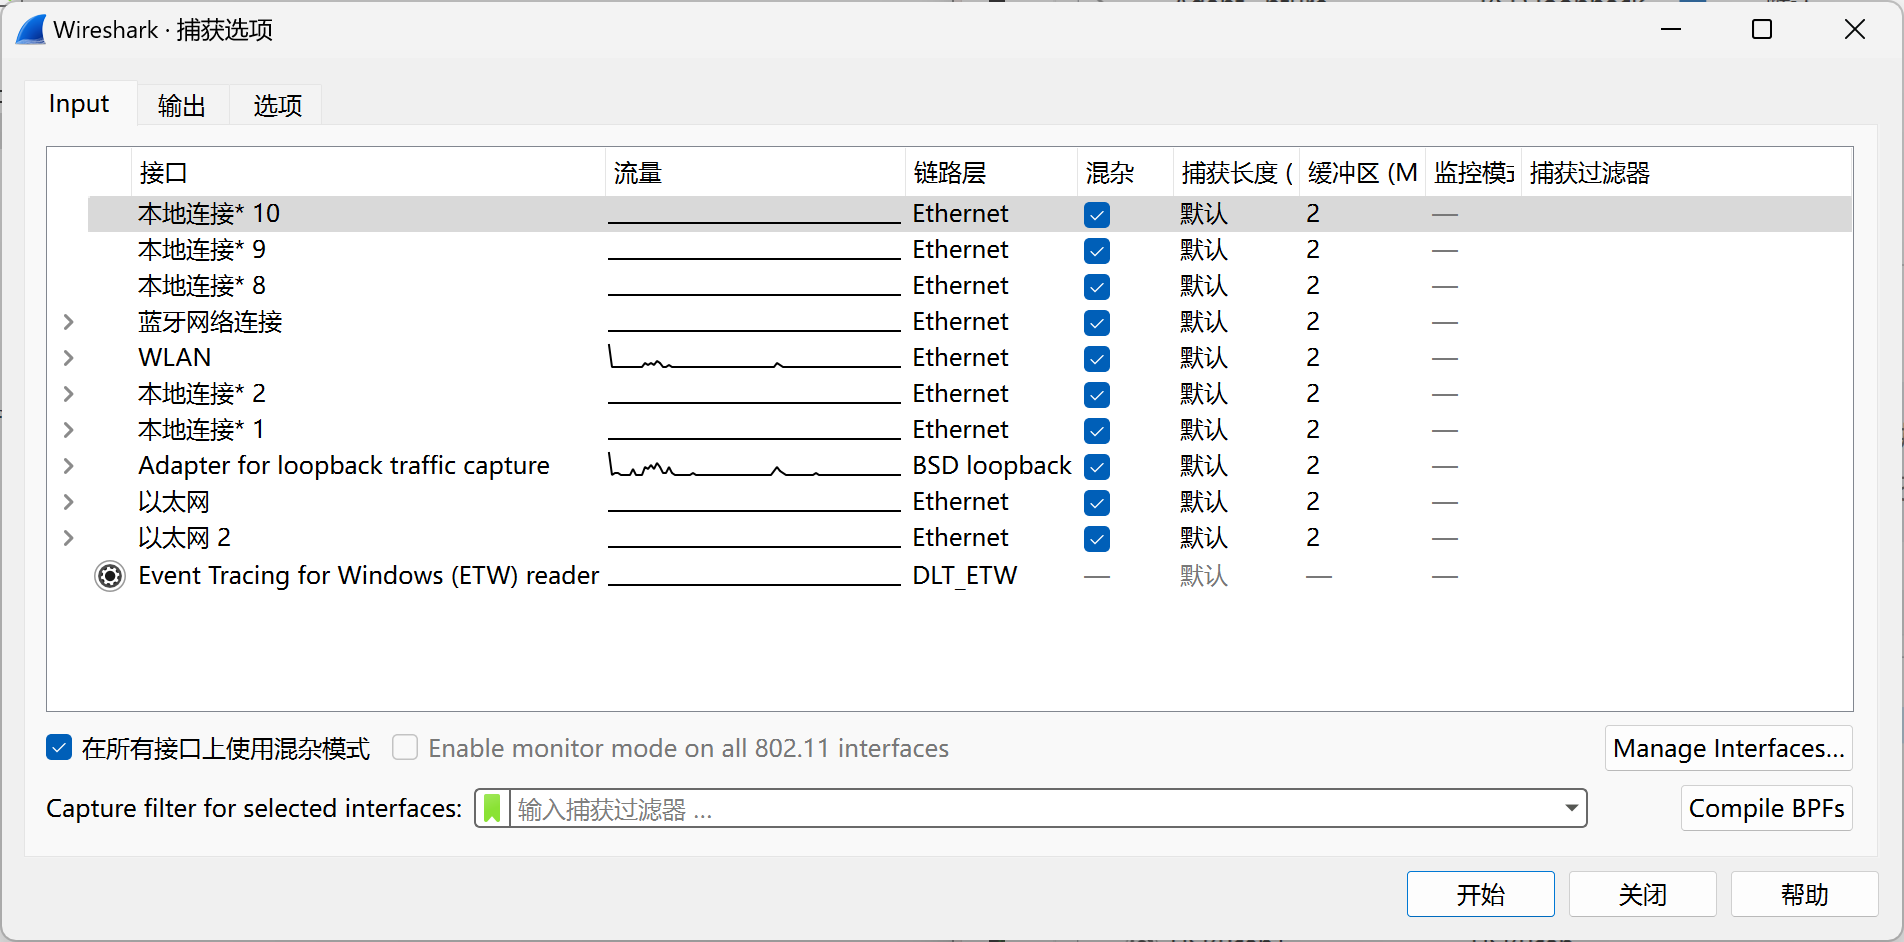
\includegraphics[width=0.8\textwidth]{1_1_images/1.png}}
\vspace{10pt}
在这个页面进行过滤器的设置,点击某个接口然后在下面输入过滤要求:
协议过滤:输入tcp进行协议过滤,筛选出所有使用TCP协议的数据包。

\vspace{10pt}
\centerline{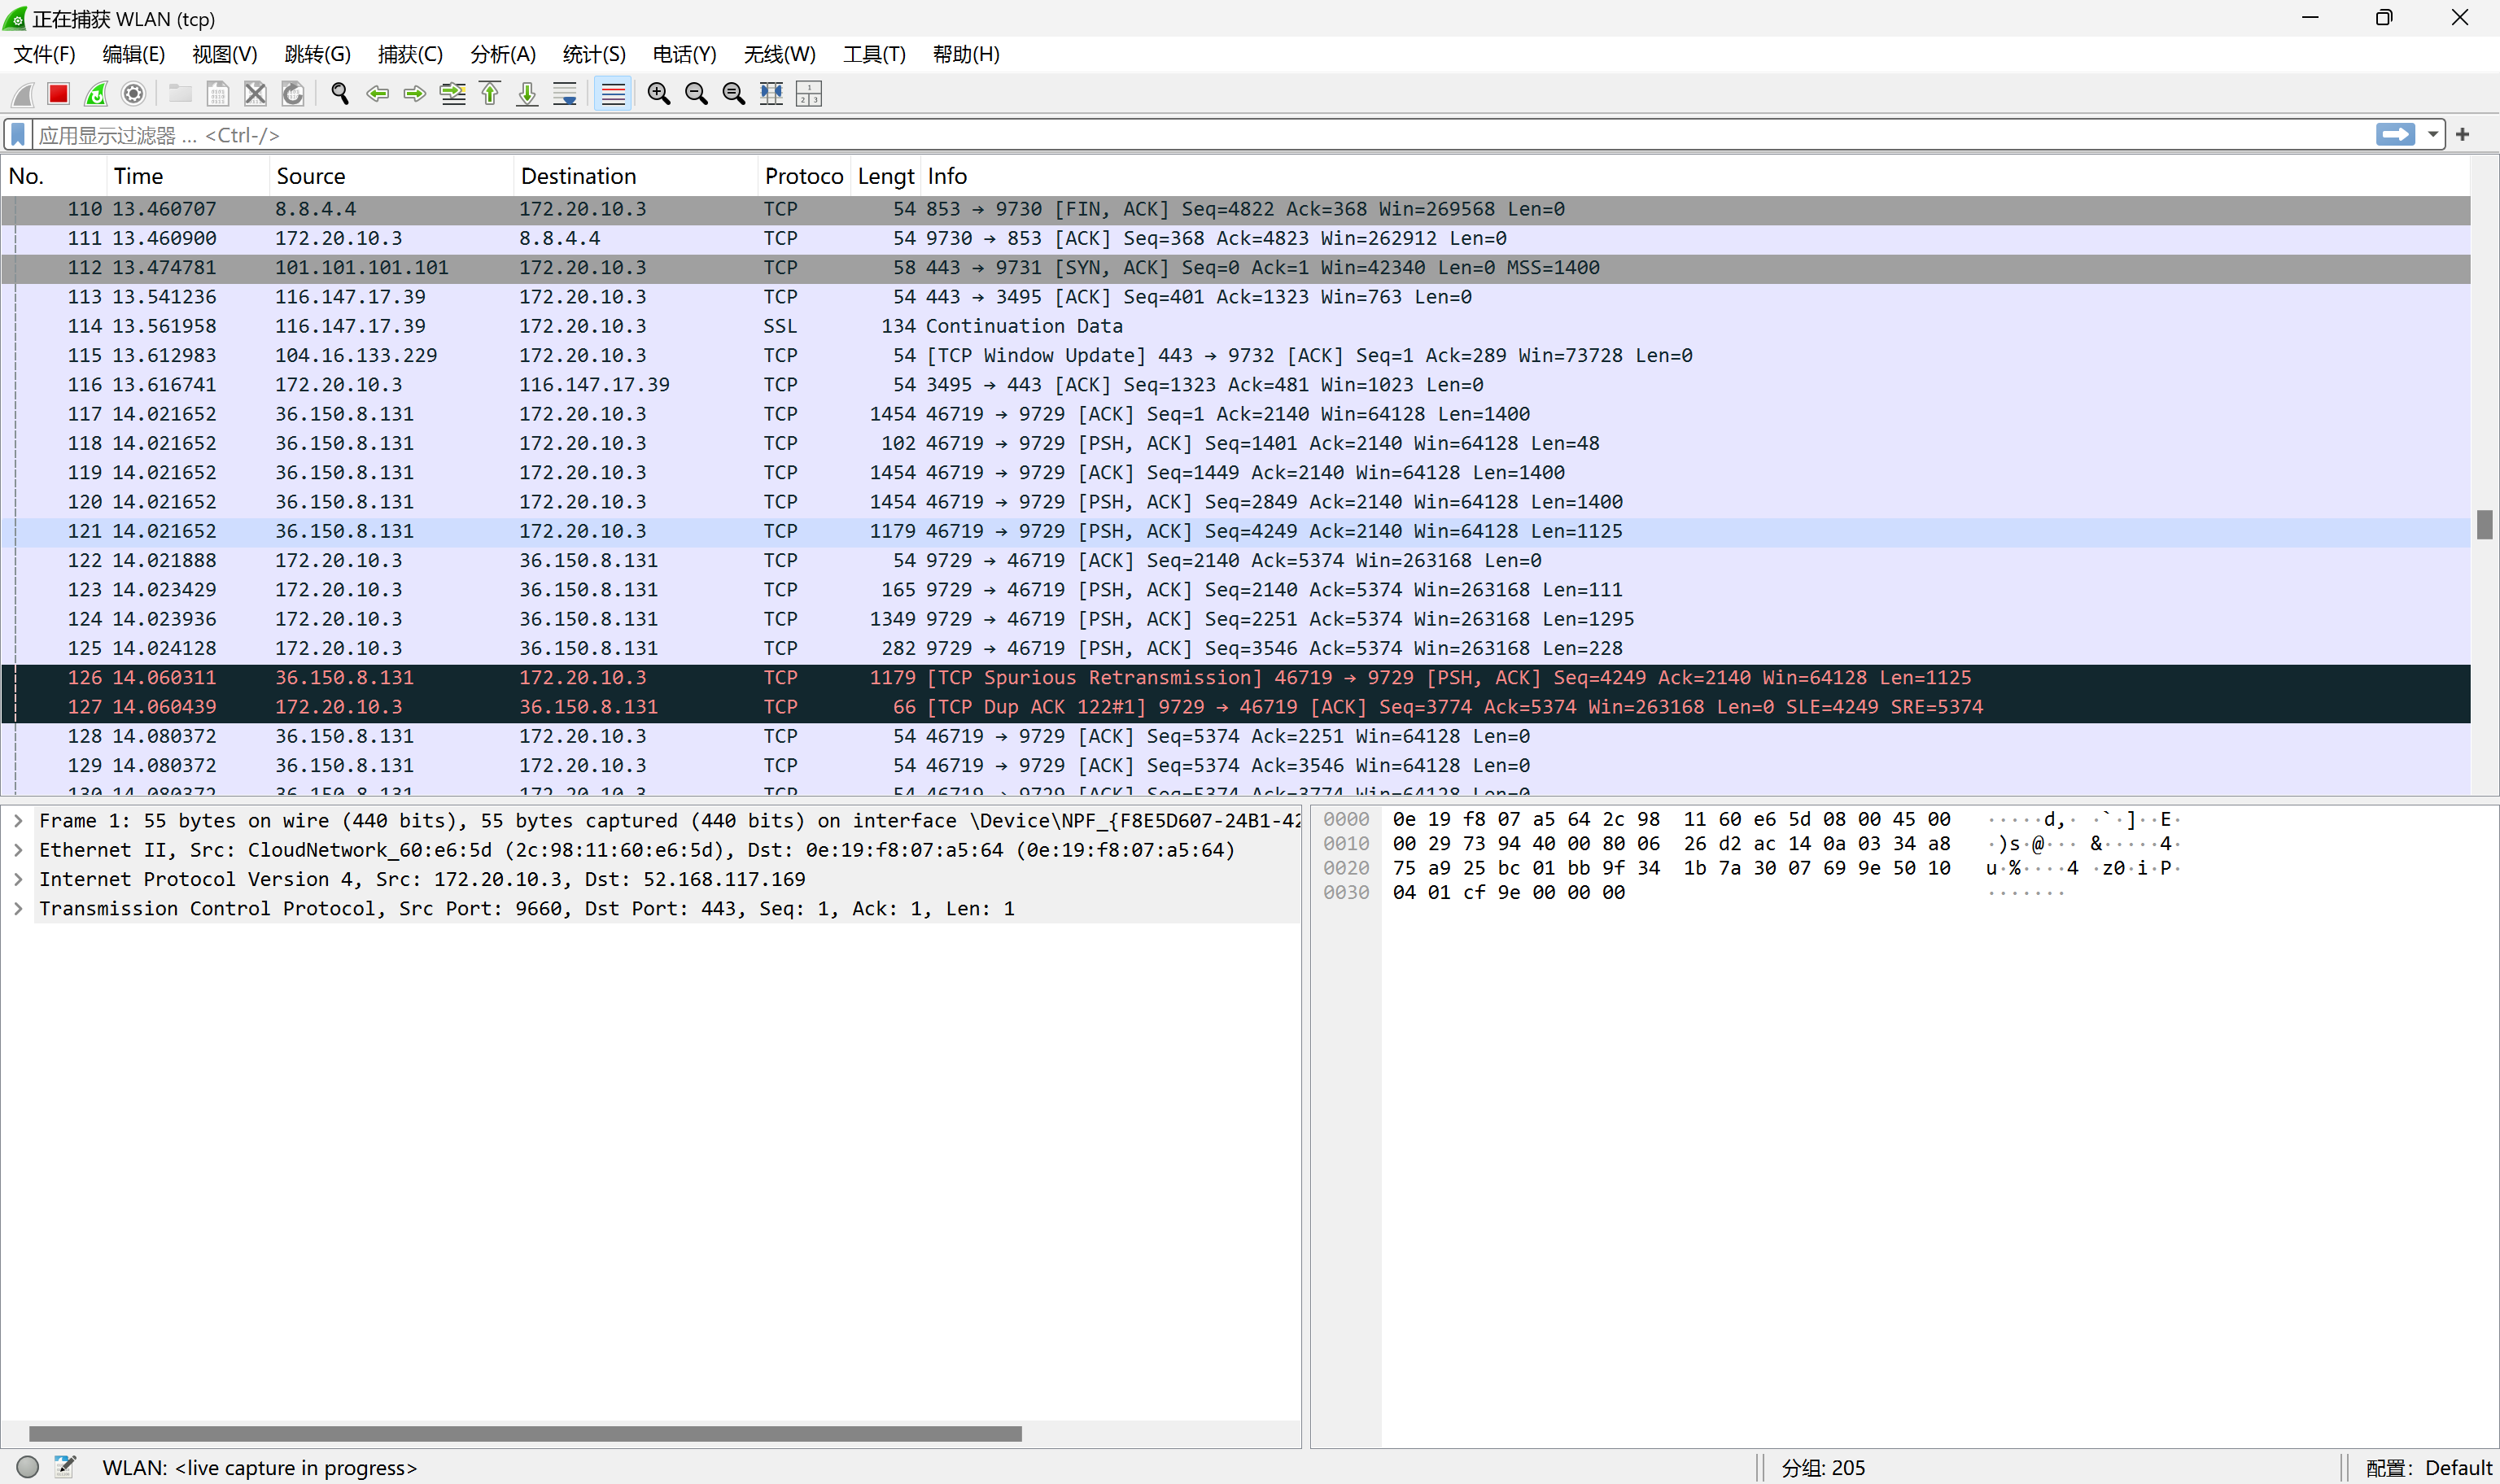
\includegraphics[width=0.8\textwidth]{1_1_images/2.png}}
\vspace{10pt}
IP过滤:输入host 192.168.5.231进行IP过滤,筛选出本机发送的数据包。

\vspace{10pt}
\centerline{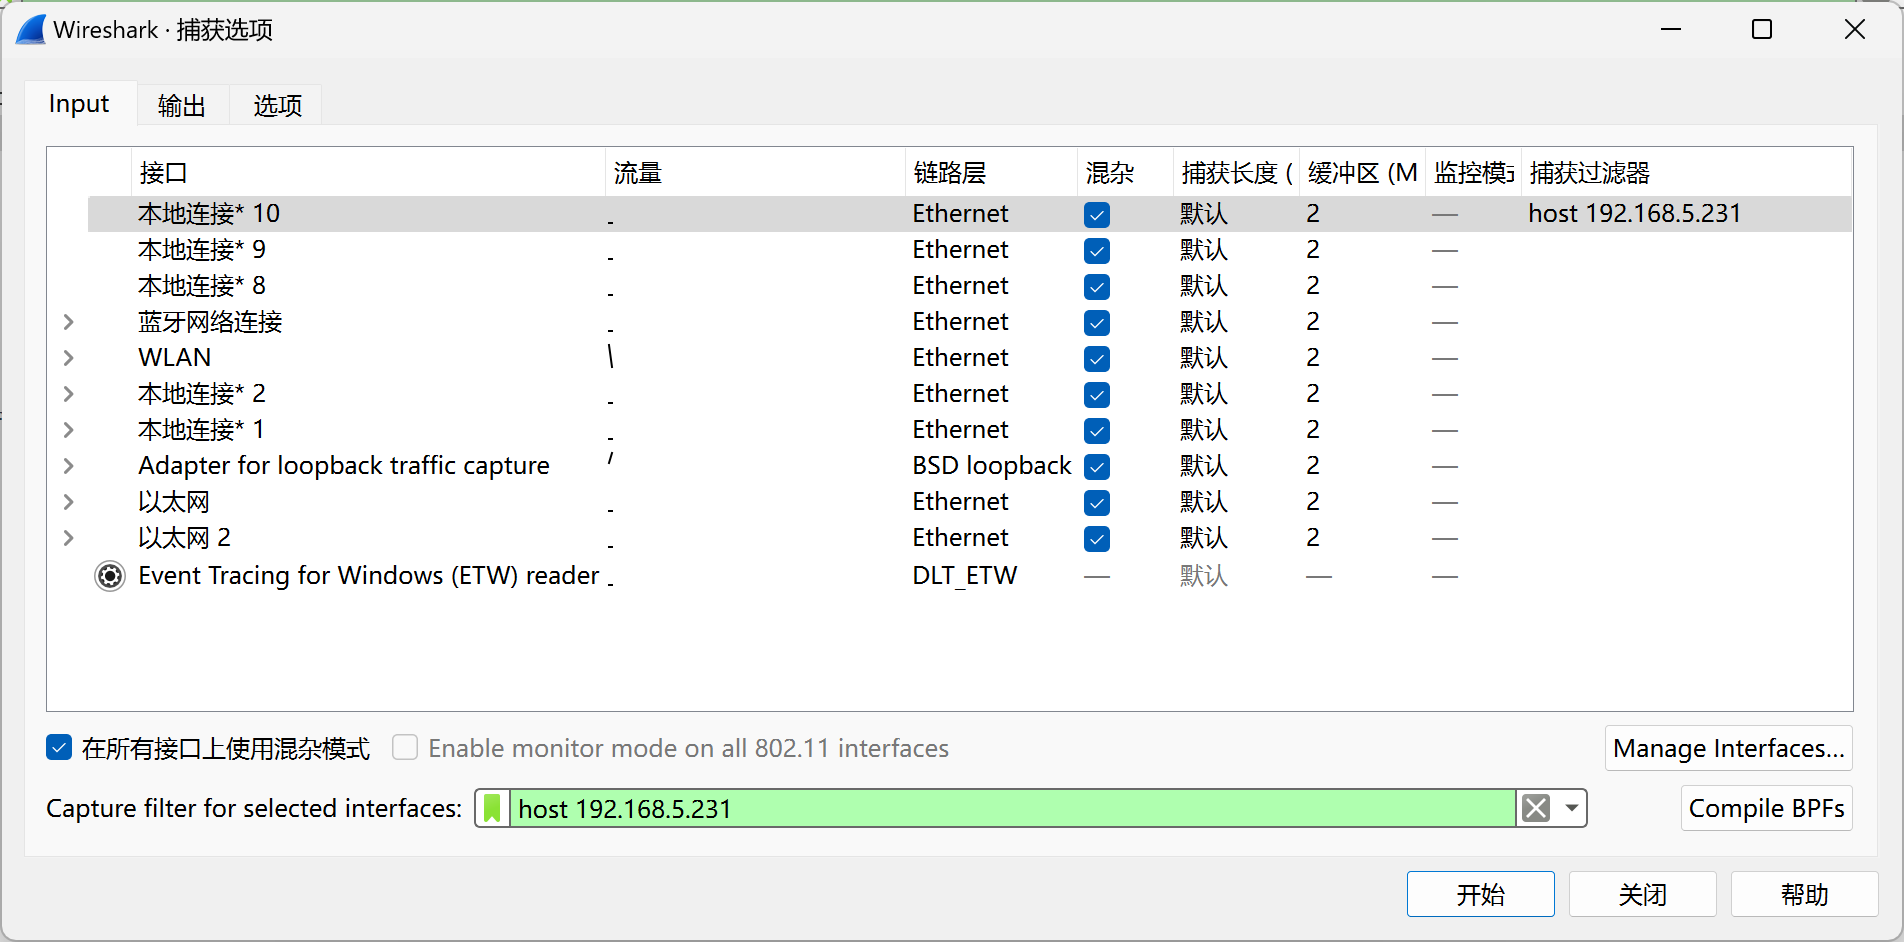
\includegraphics[width=0.8\textwidth]{1_1_images/3.png}}
\vspace{10pt}
端口过滤:输入port 80进行端口过滤,筛选出本机发送的数据包。

\vspace{10pt}
\centerline{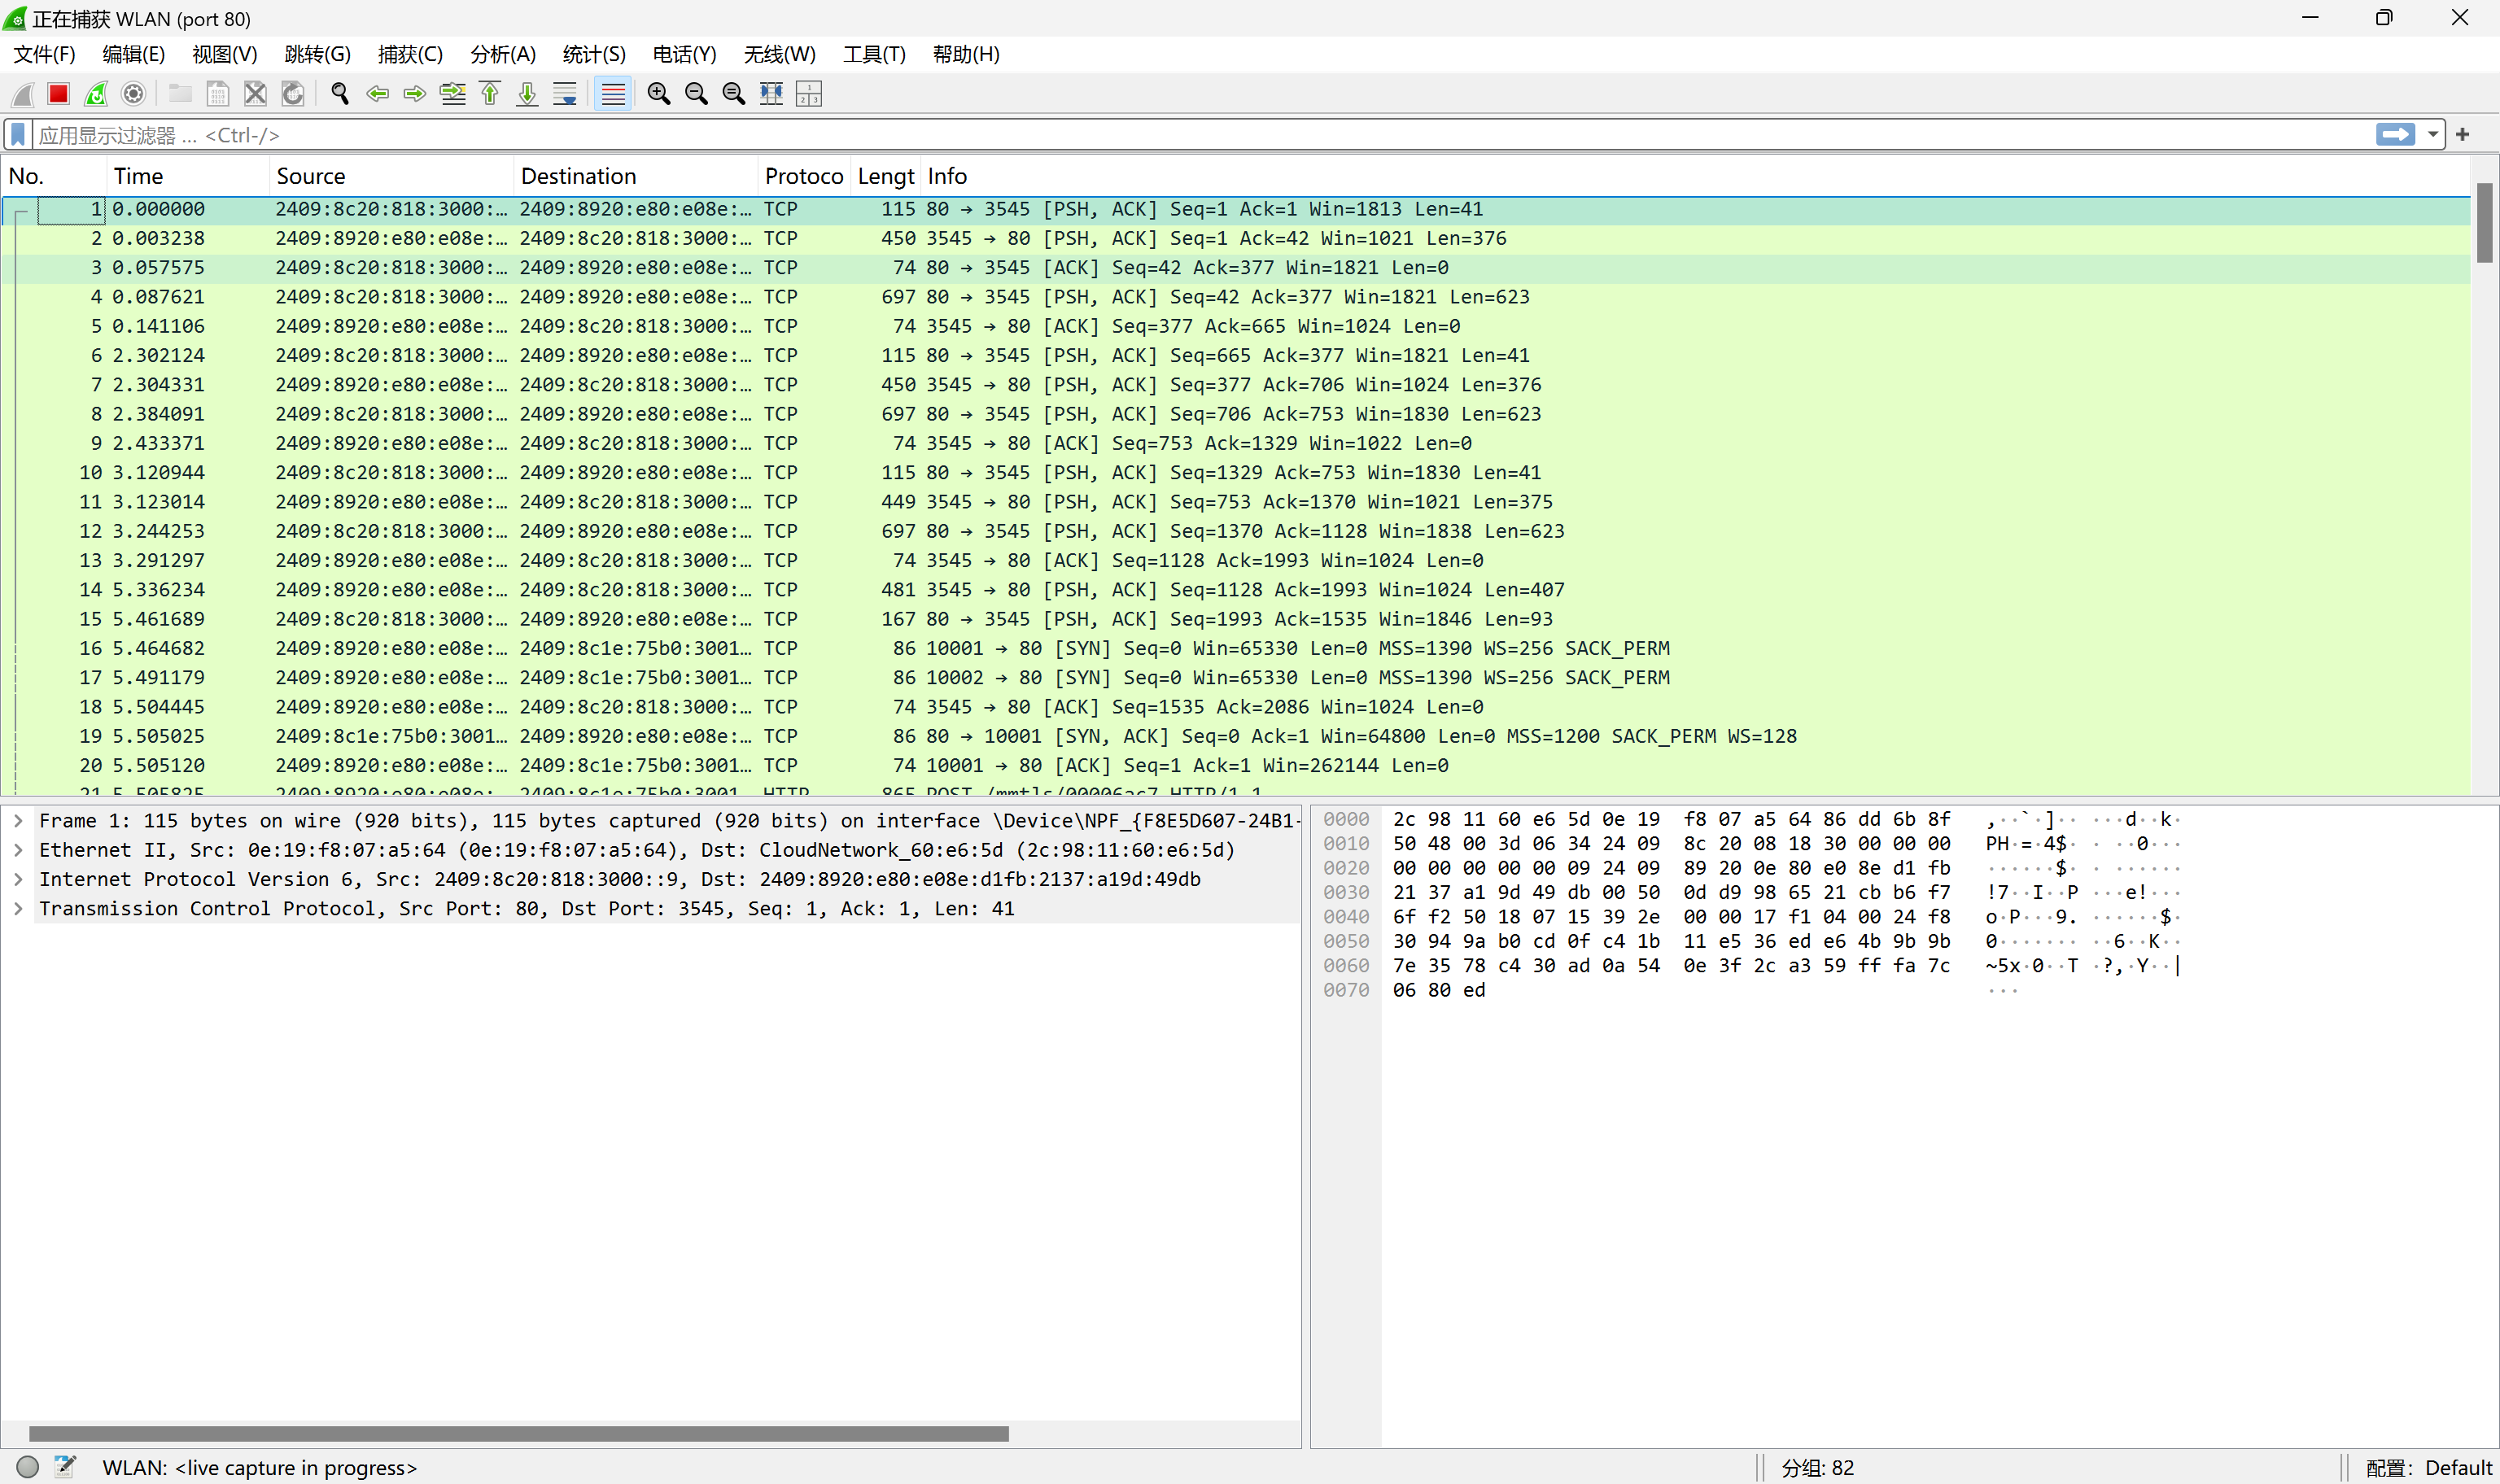
\includegraphics[width=0.8\textwidth]{1_1_images/4.png}}
\vspace{10pt}

\textbf{(2)在开始抓包后设置过滤条件:}
在开始捕获后,可以再次设置过滤器:

\vspace{10pt}
\centerline{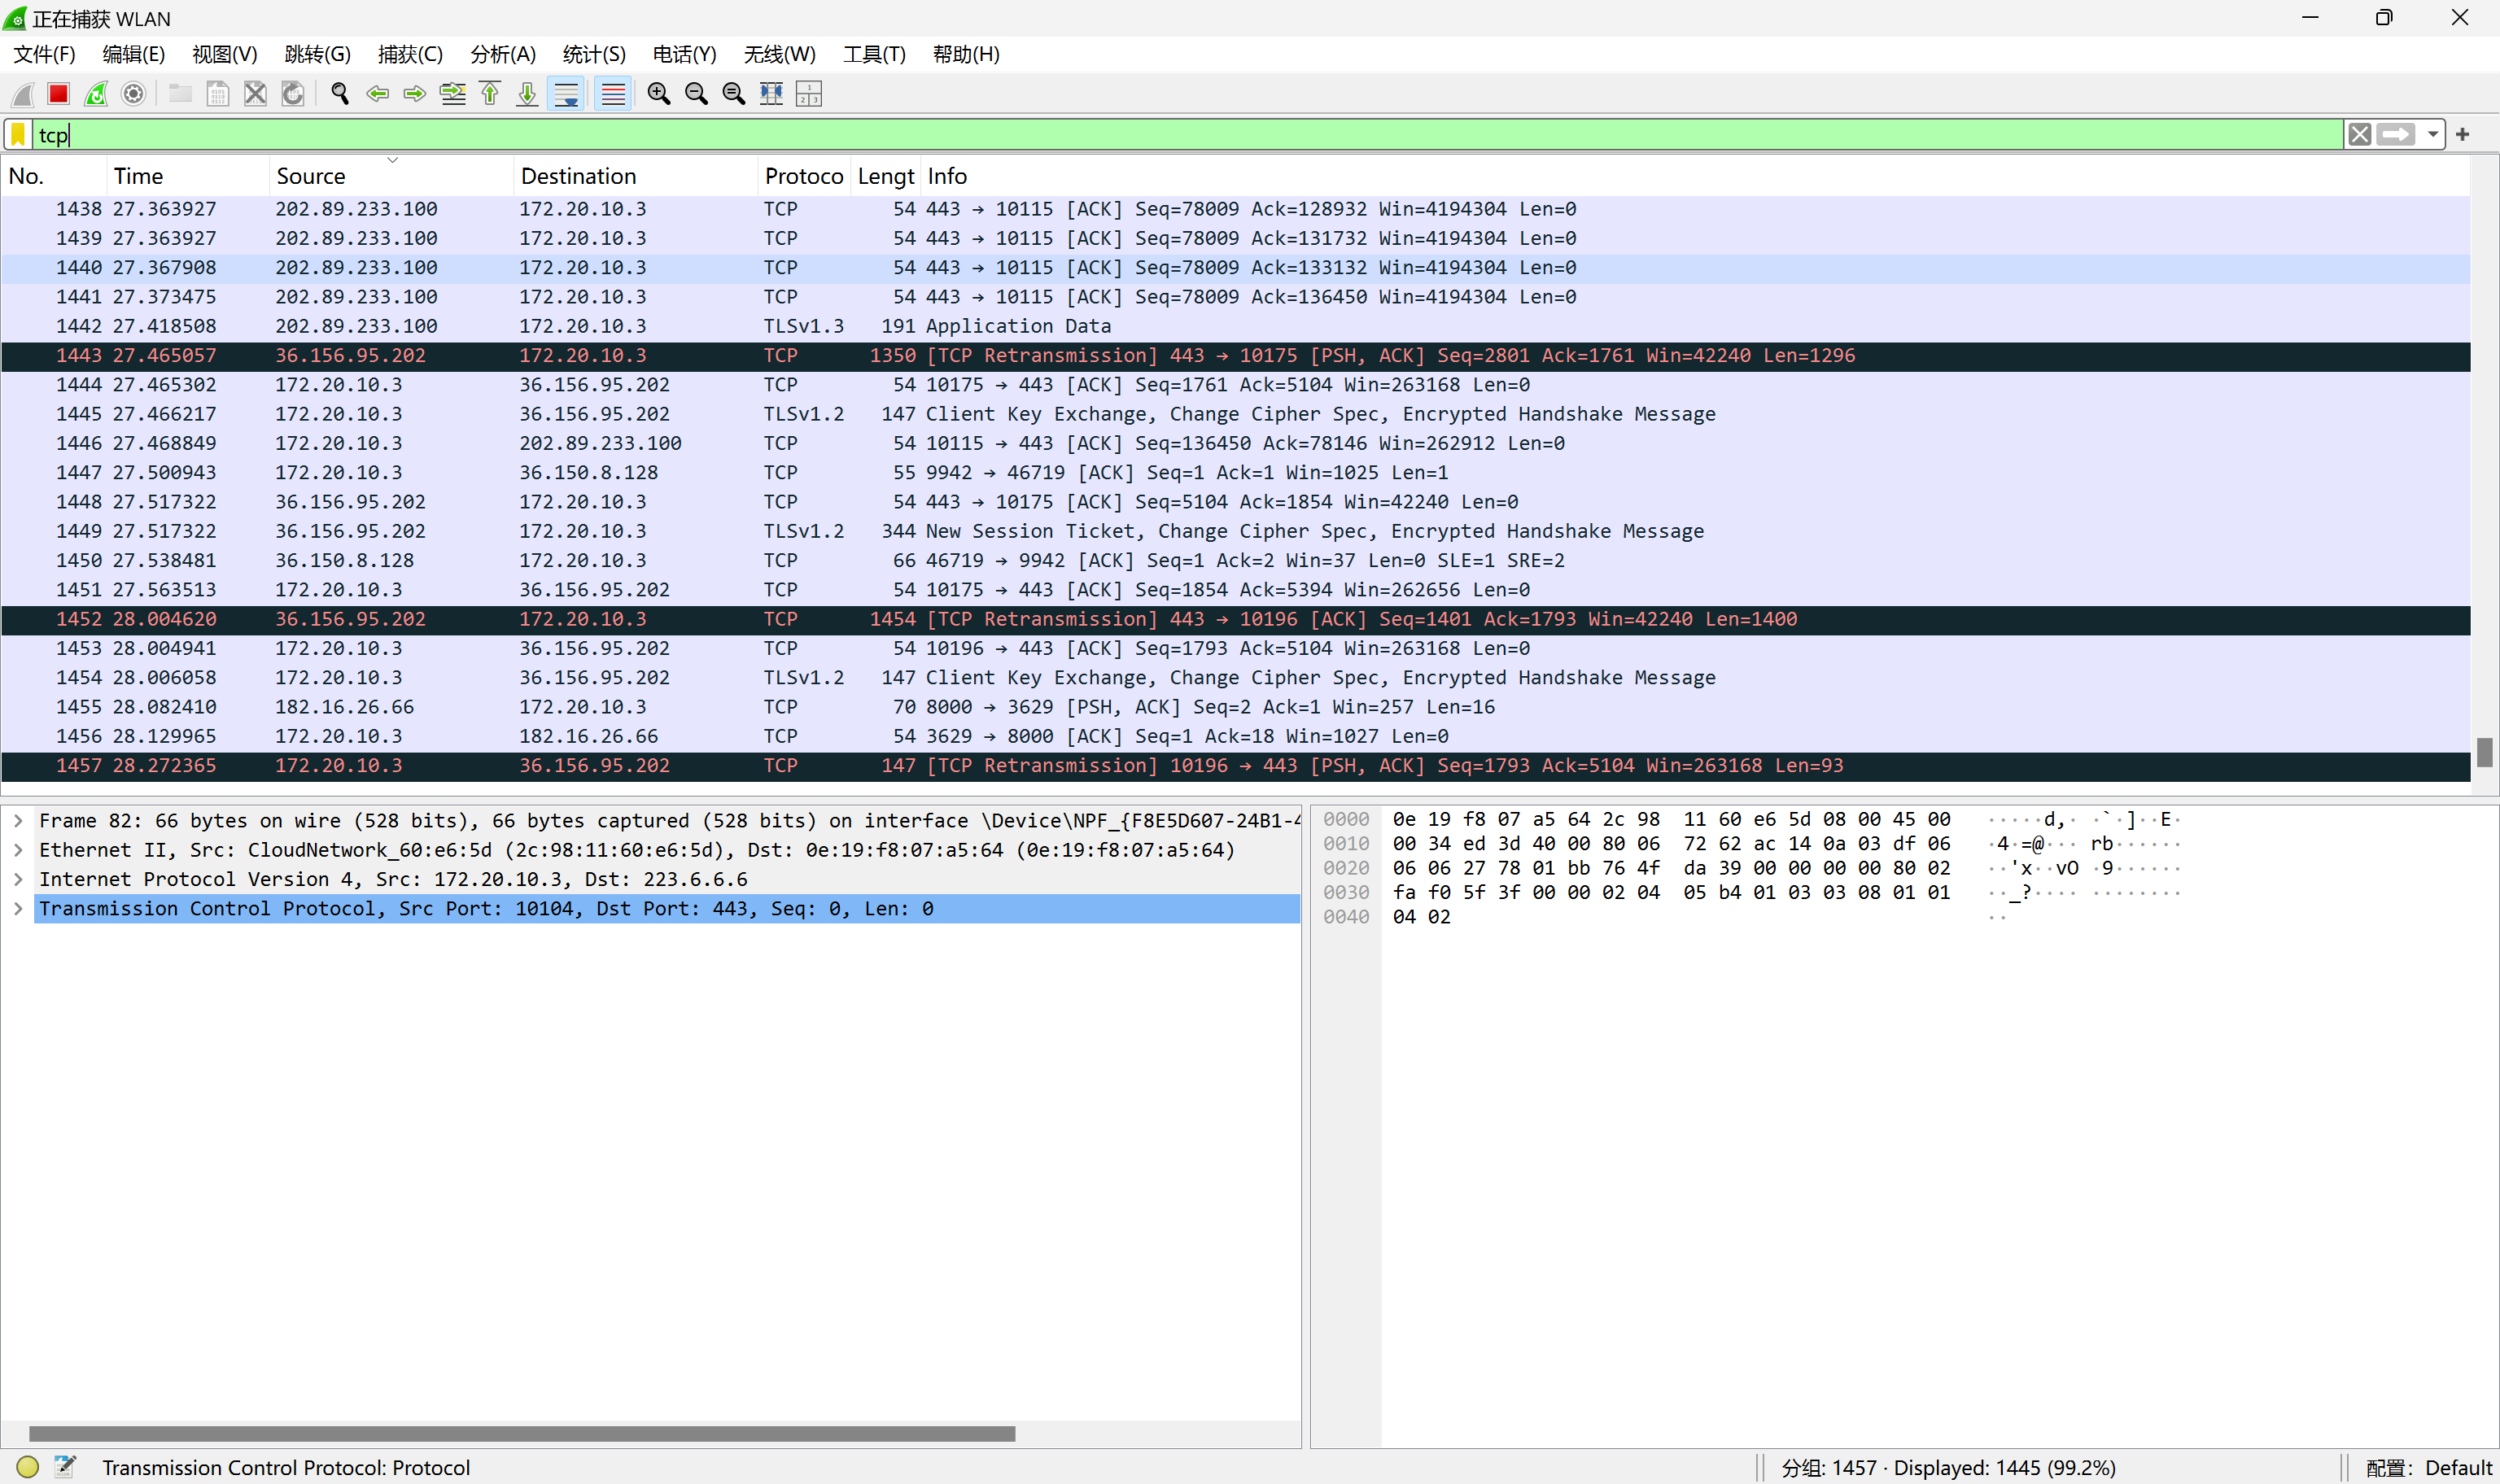
\includegraphics[width=0.8\textwidth]{1_1_images/5.png}}
\vspace{10pt}

\vspace{10pt}
\centerline{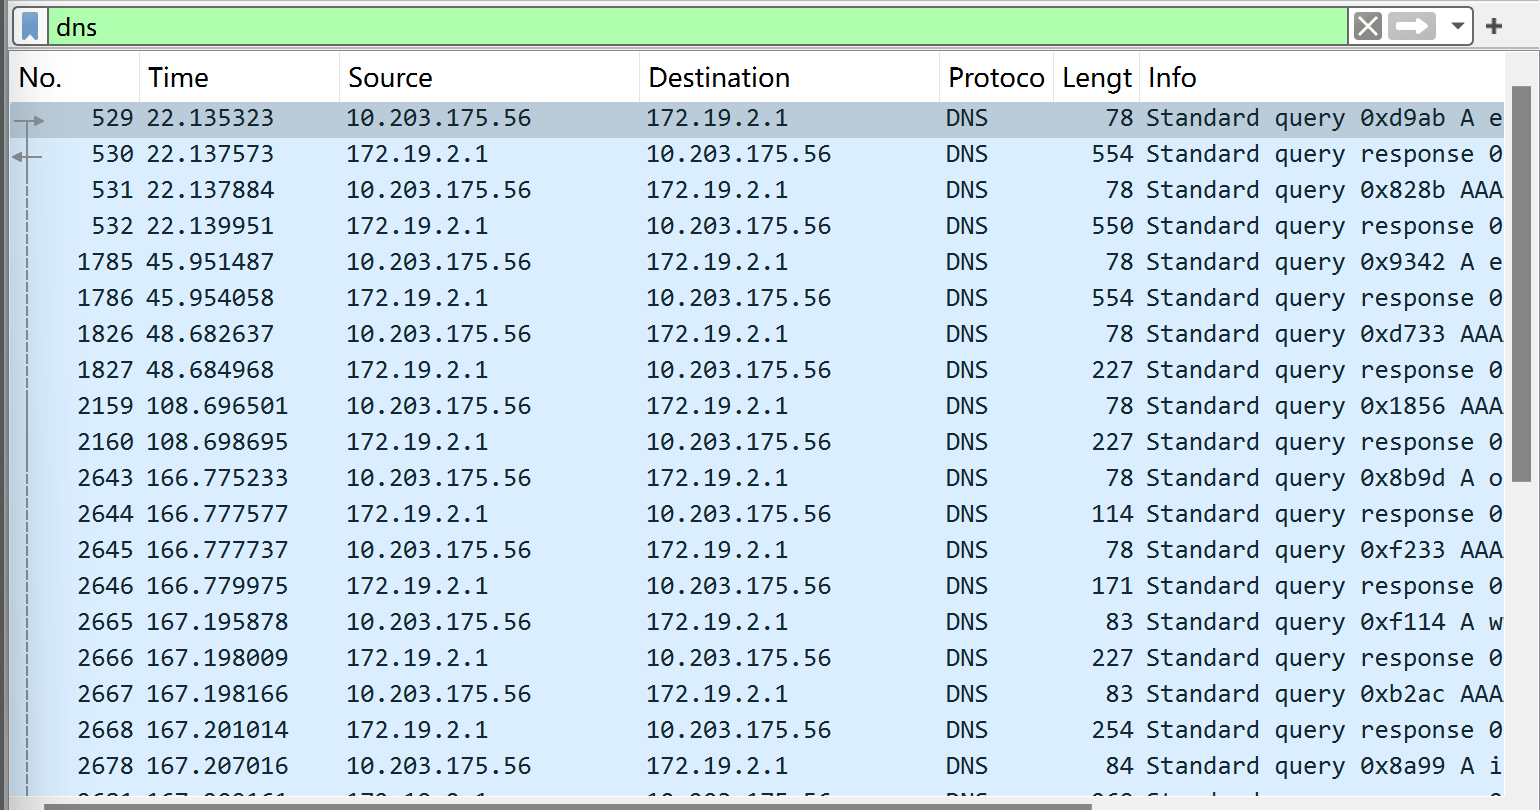
\includegraphics[width=0.8\textwidth]{1_1_images/6.png}}
\vspace{10pt}

\vspace{10pt}
\centerline{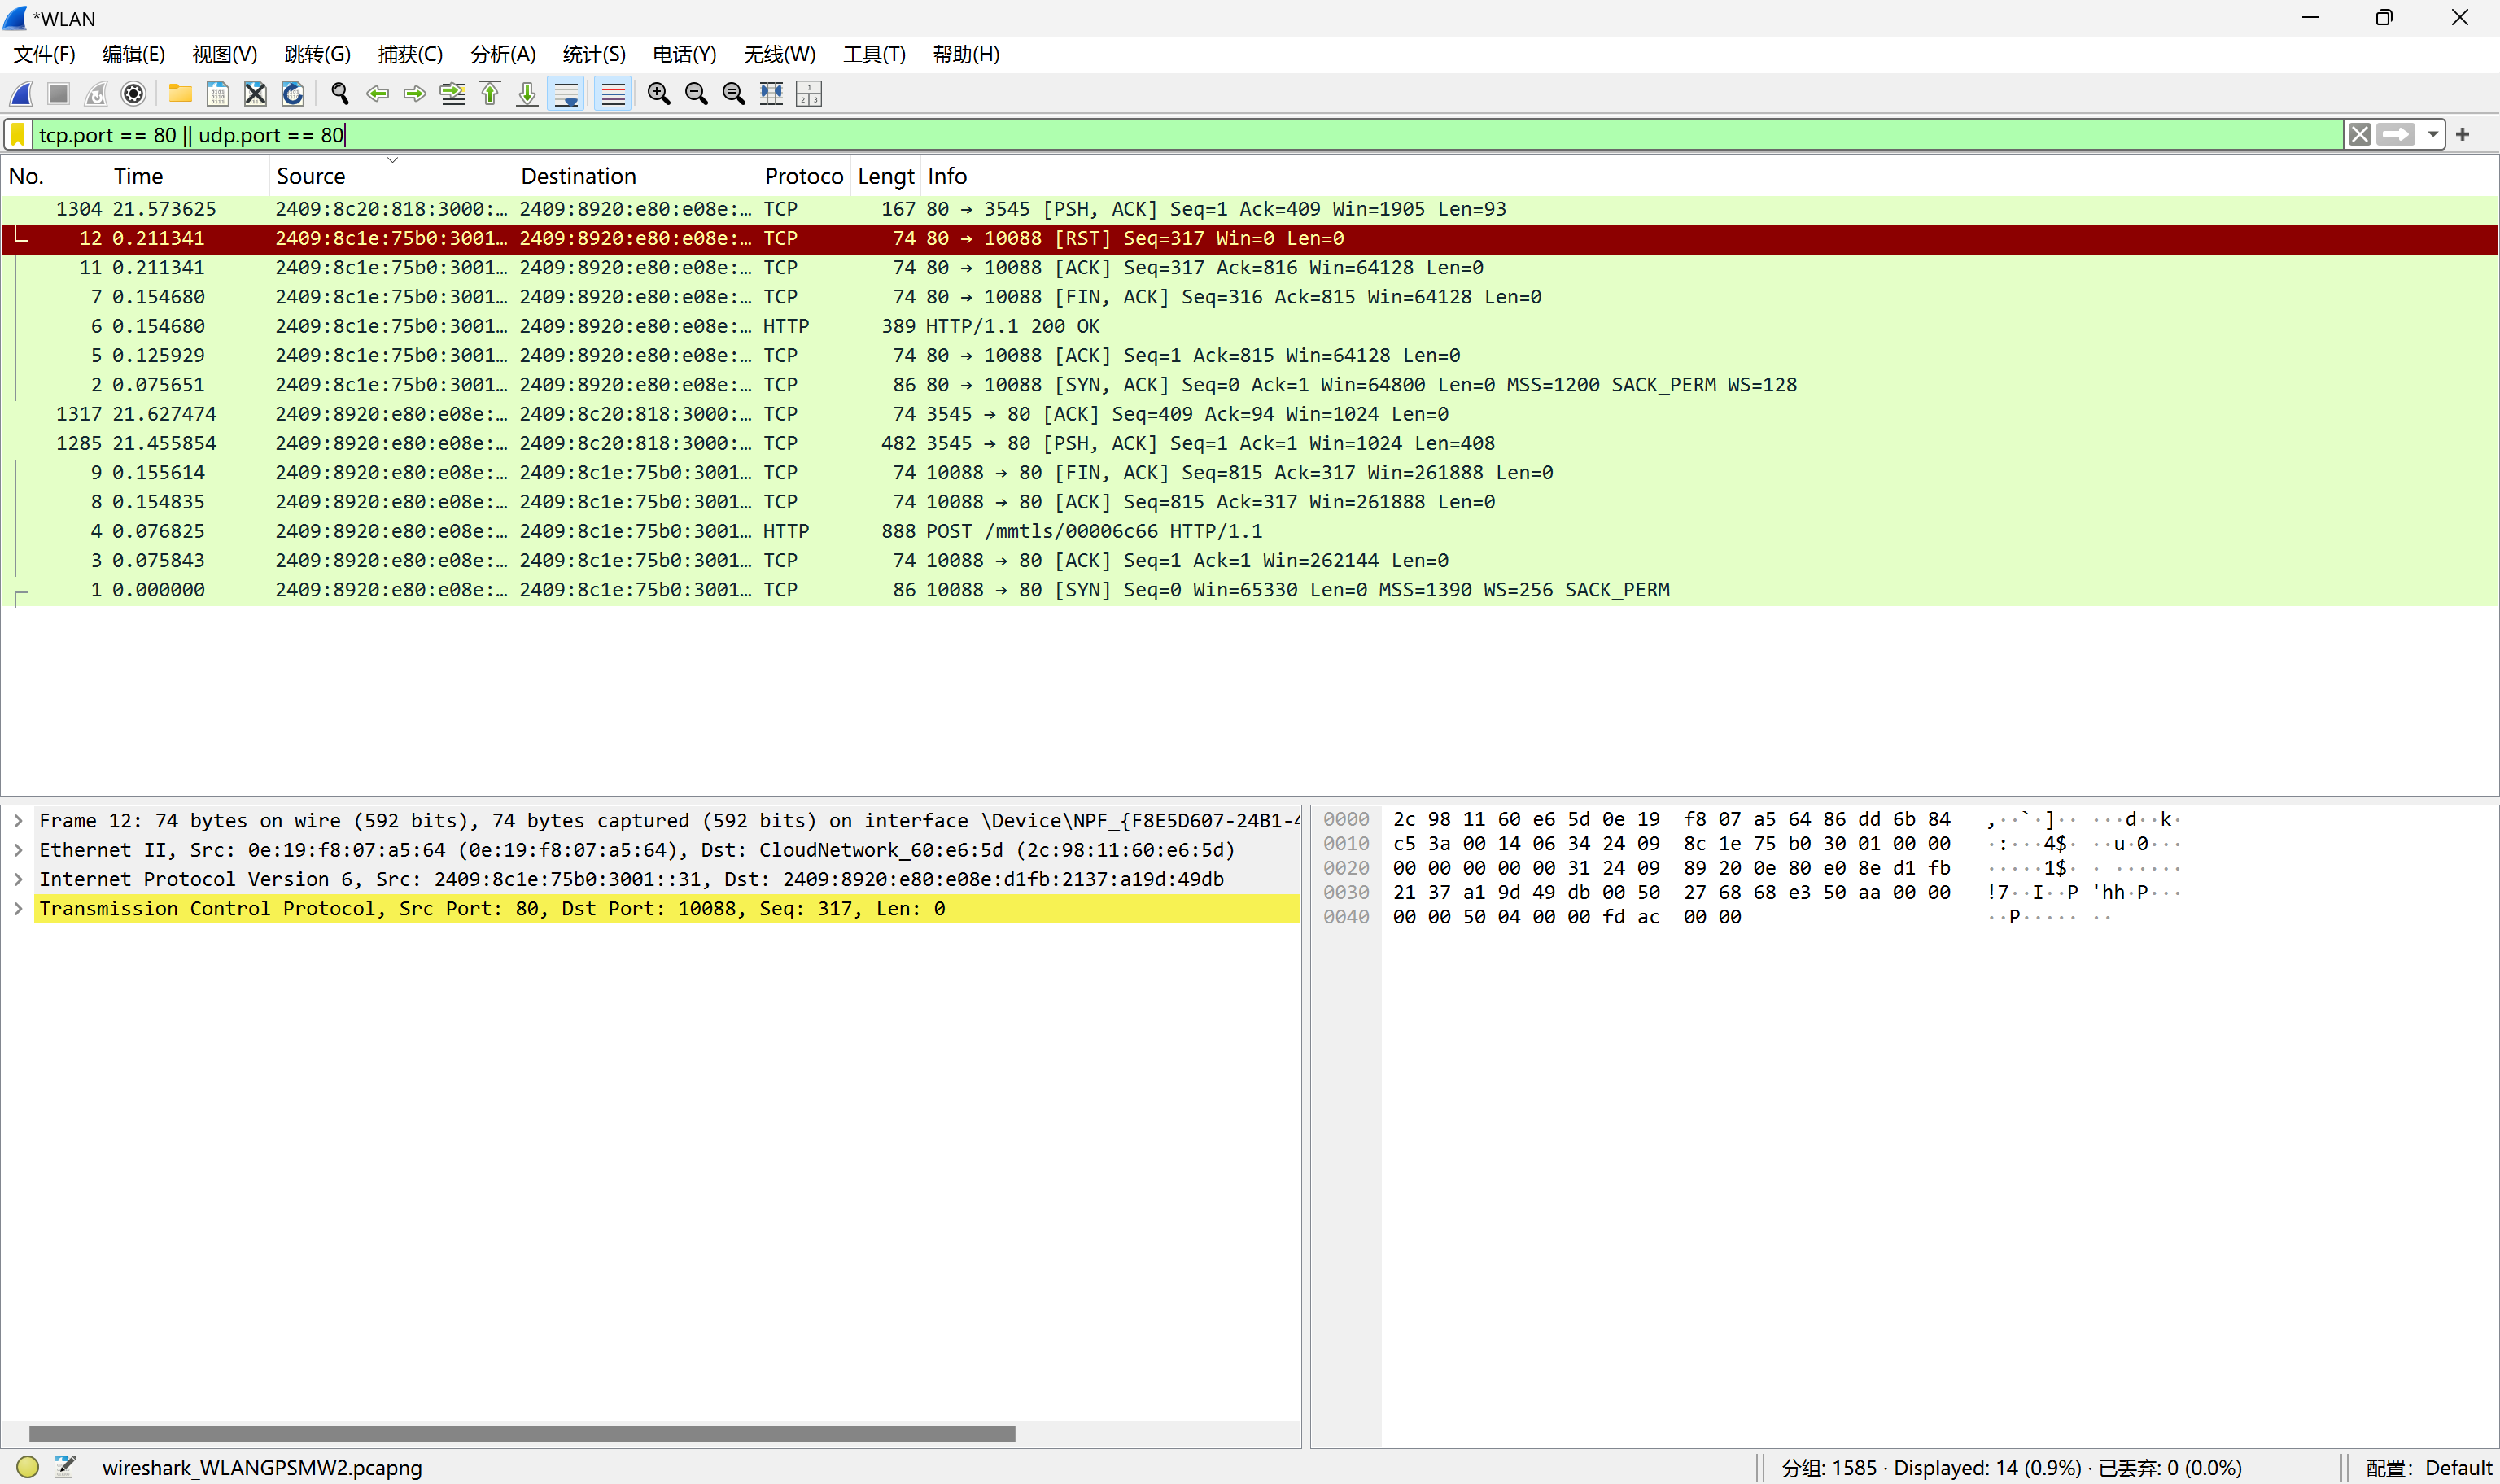
\includegraphics[width=0.8\textwidth]{1_1_images/7.png}}
\vspace{10pt}

\subsubsection{学习 Wireshark 基本操作。}

利用网络打开某个网页,或者进行收发消息的操作,可以在列表中看到新的相应数据包,然后把筛选条件分别改为http和dns,查看对应的协议内容:

\vspace{10pt}
\centerline{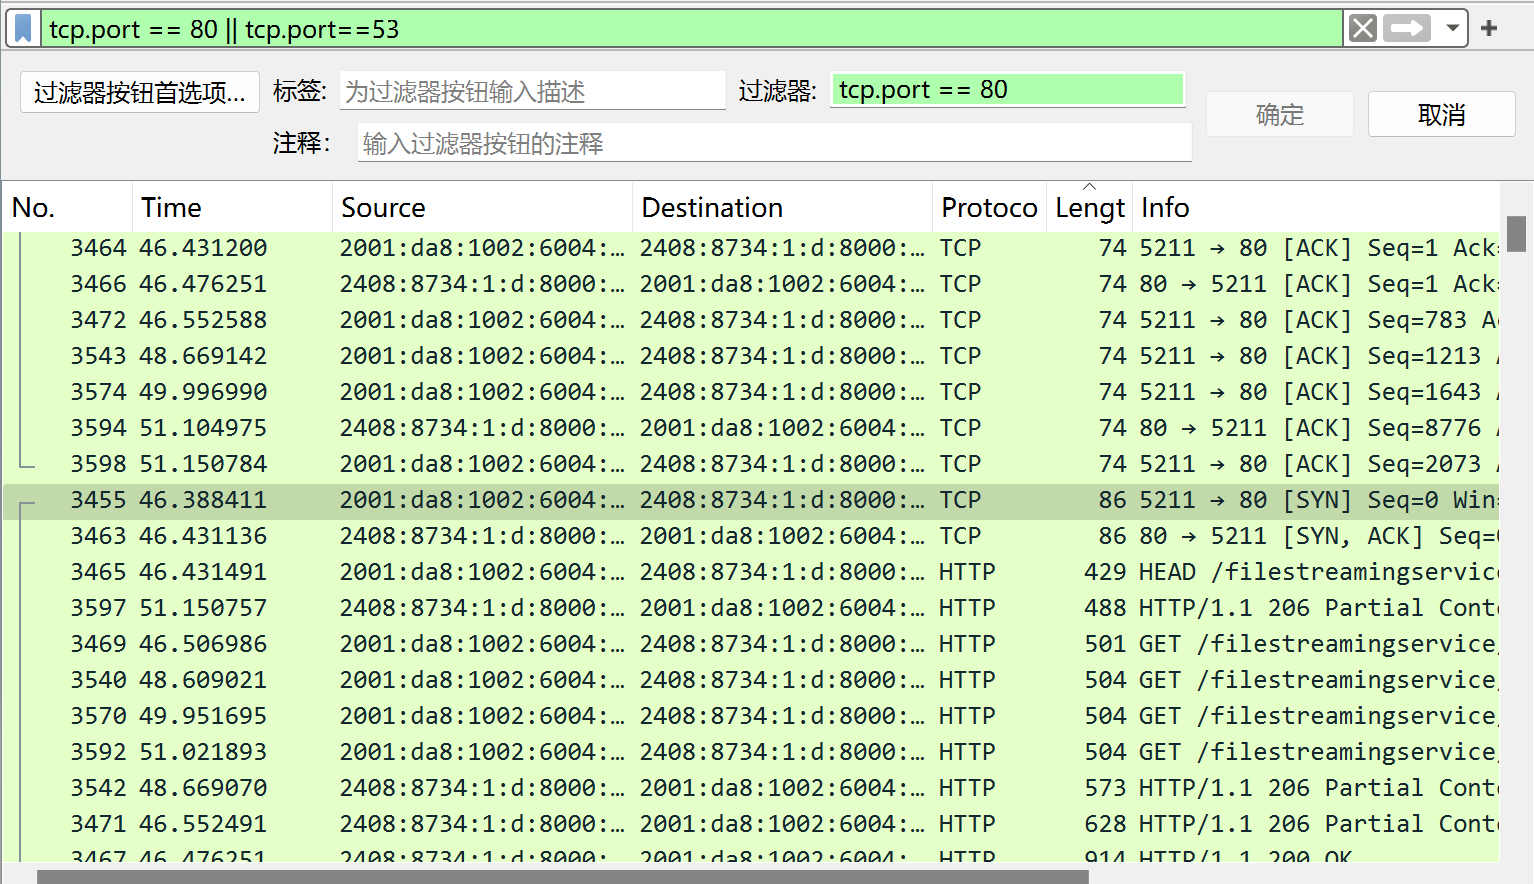
\includegraphics[width=0.8\textwidth]{1_1_images/8.png}}
\vspace{10pt}
HTTP协议:

\vspace{10pt}
\centerline{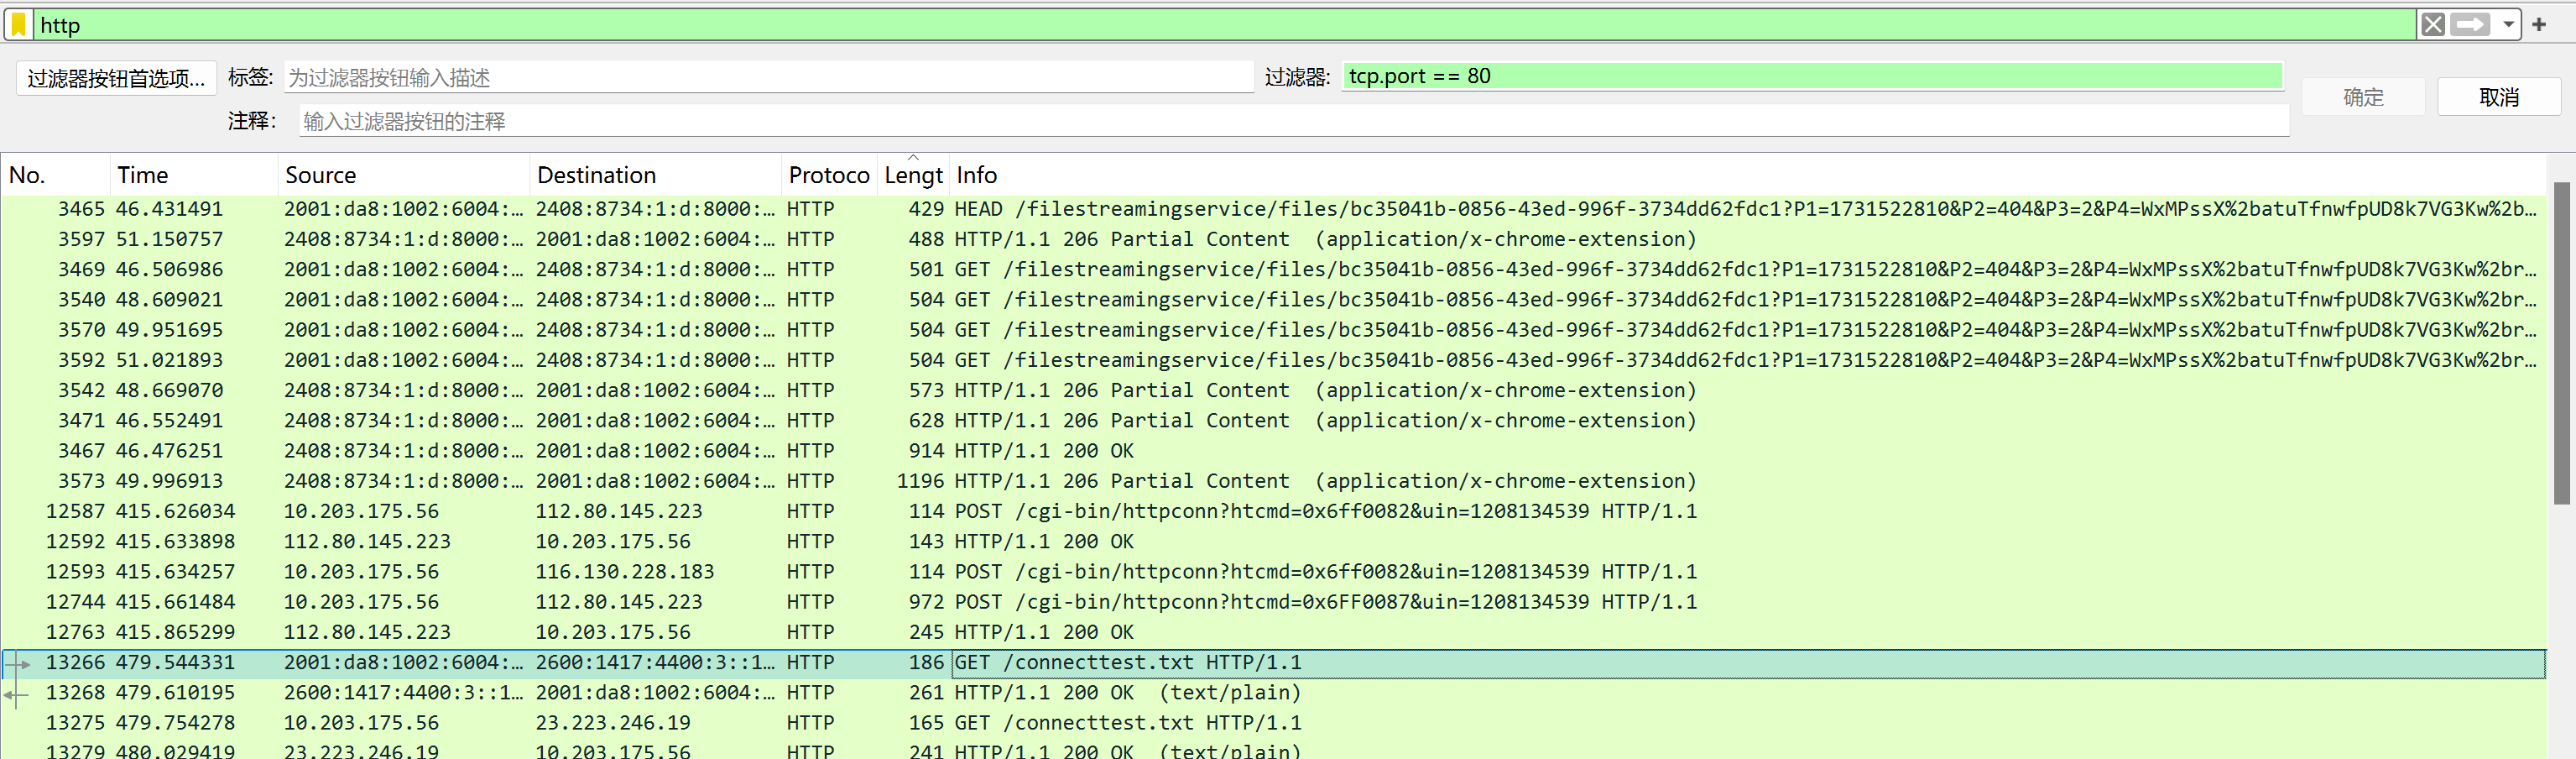
\includegraphics[width=0.8\textwidth]{1_1_images/9.png}}
\vspace{10pt}
基于HTTP报文格式对此进行分析:

第一行是请求行,表明采用GET方法,使用HTTP1.1版本协议,请求资源路径是根目录。

第二行是首部行,Host表明请求的目标服务器的域名,User-Agent:Mozilla/5.0(Windows NT 10.0; Win64; x64) AppleWebKit/537.36(KHTML, like Gecko) Chrome/126,客户端浏览器的标识信息。Accept:客户端能够处理的媒体类型。Accept-Encoding:客户端支持的压缩编码,Accept-Language:客户端偏好的语言。Cookie:客户端存储的服务器发送的cookie。

DNS协议:

\vspace{10pt}
\centerline{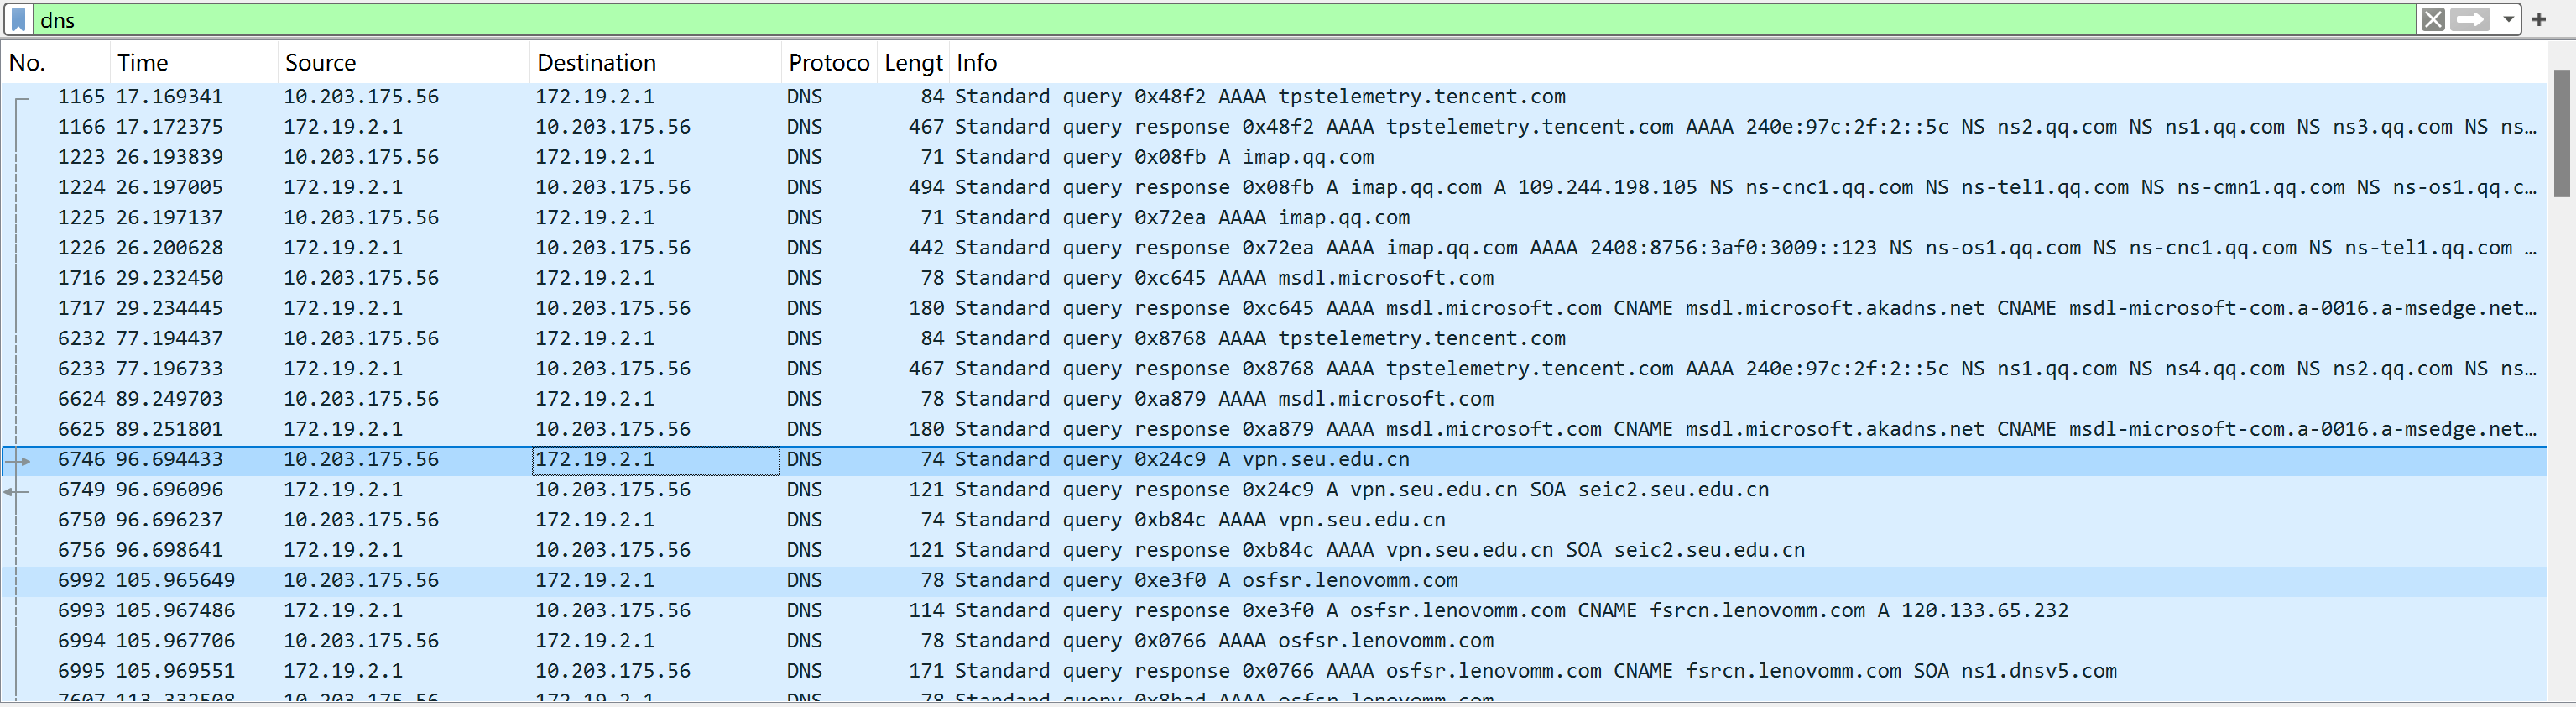
\includegraphics[width=0.8\textwidth]{1_1_images/10.png}}
\vspace{10pt}

\vspace{10pt}
\centerline{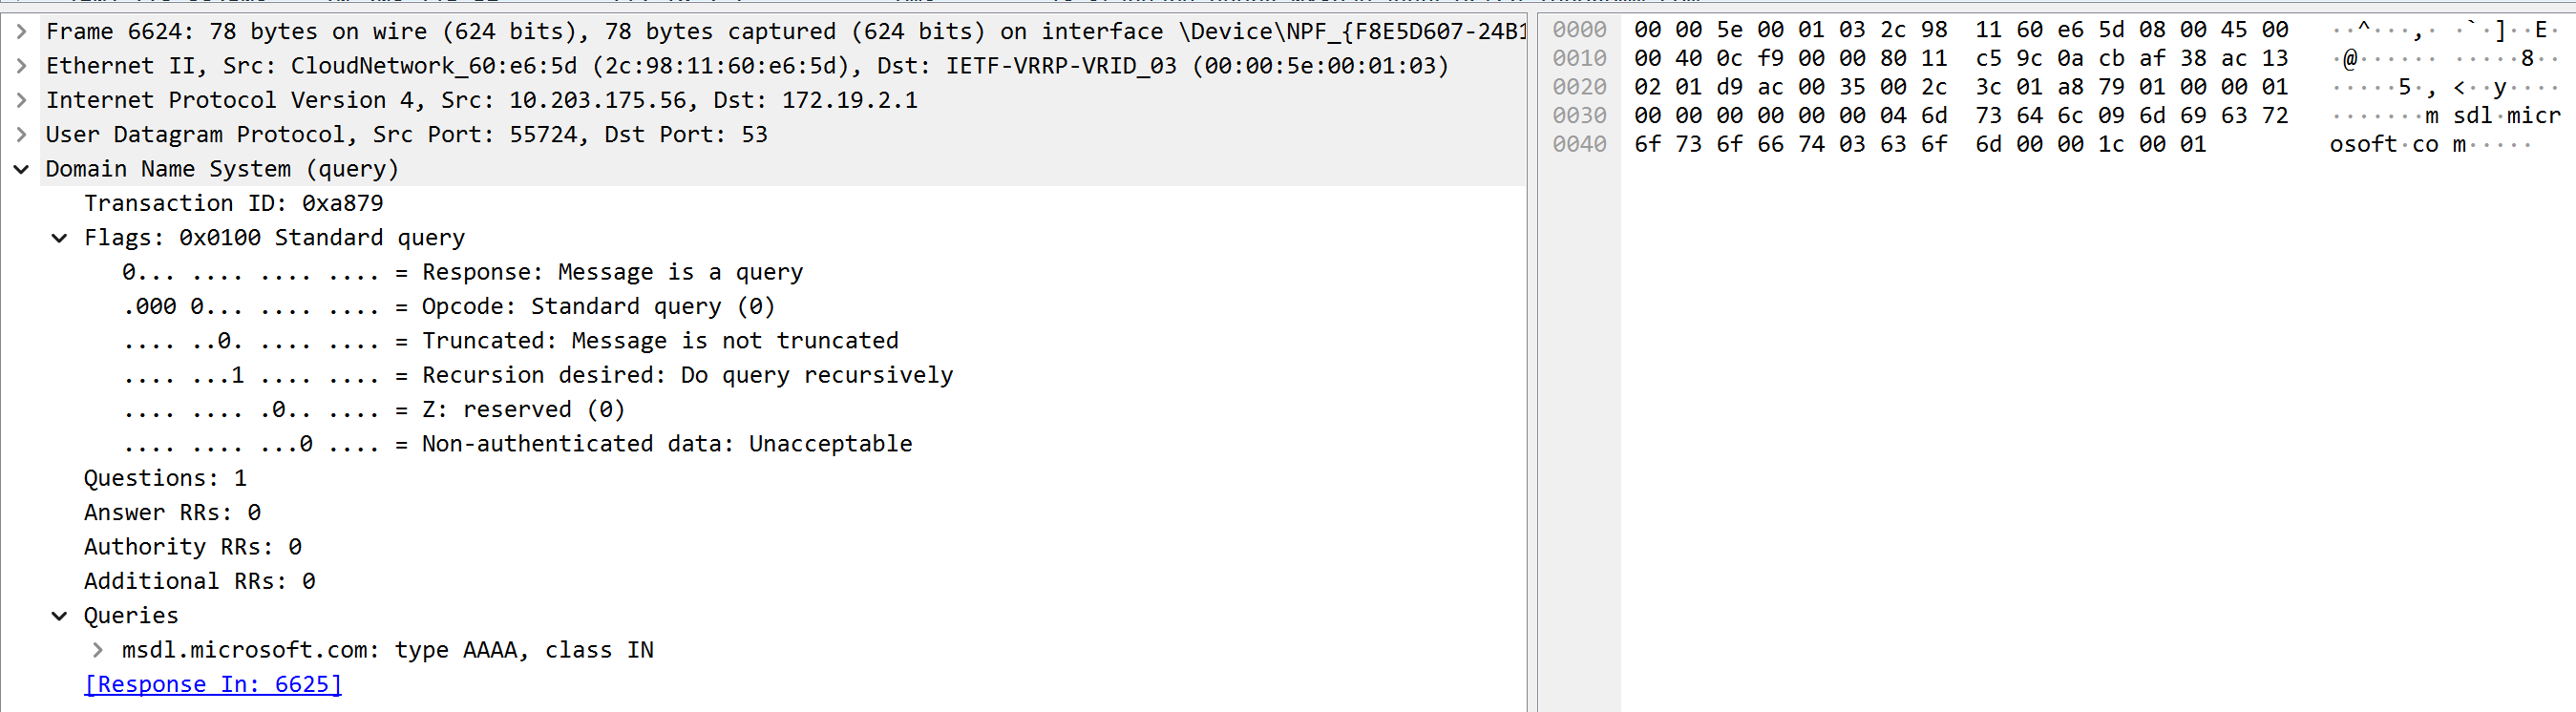
\includegraphics[width=0.8\textwidth]{1_1_images/11.png}}
\vspace{10pt}

基于DNS报文格式对此进行分析:

查询的是msdl.microsoft.com的IPv6地址(AAAA记录)。这个查询是由IP地址为10.203.175.56的设备发出,发送到DNS服务器172.19.2.1的53端口。这个查询是一个标准查询,请求递归解析,并且没有包含任何回答、权威或额外的资源记录。
\subsubsection{测试curl命令,访问一个web页面。}

首先在命令行中执行curl www.baidu.com的访问命令:

\vspace{10pt}
\centerline{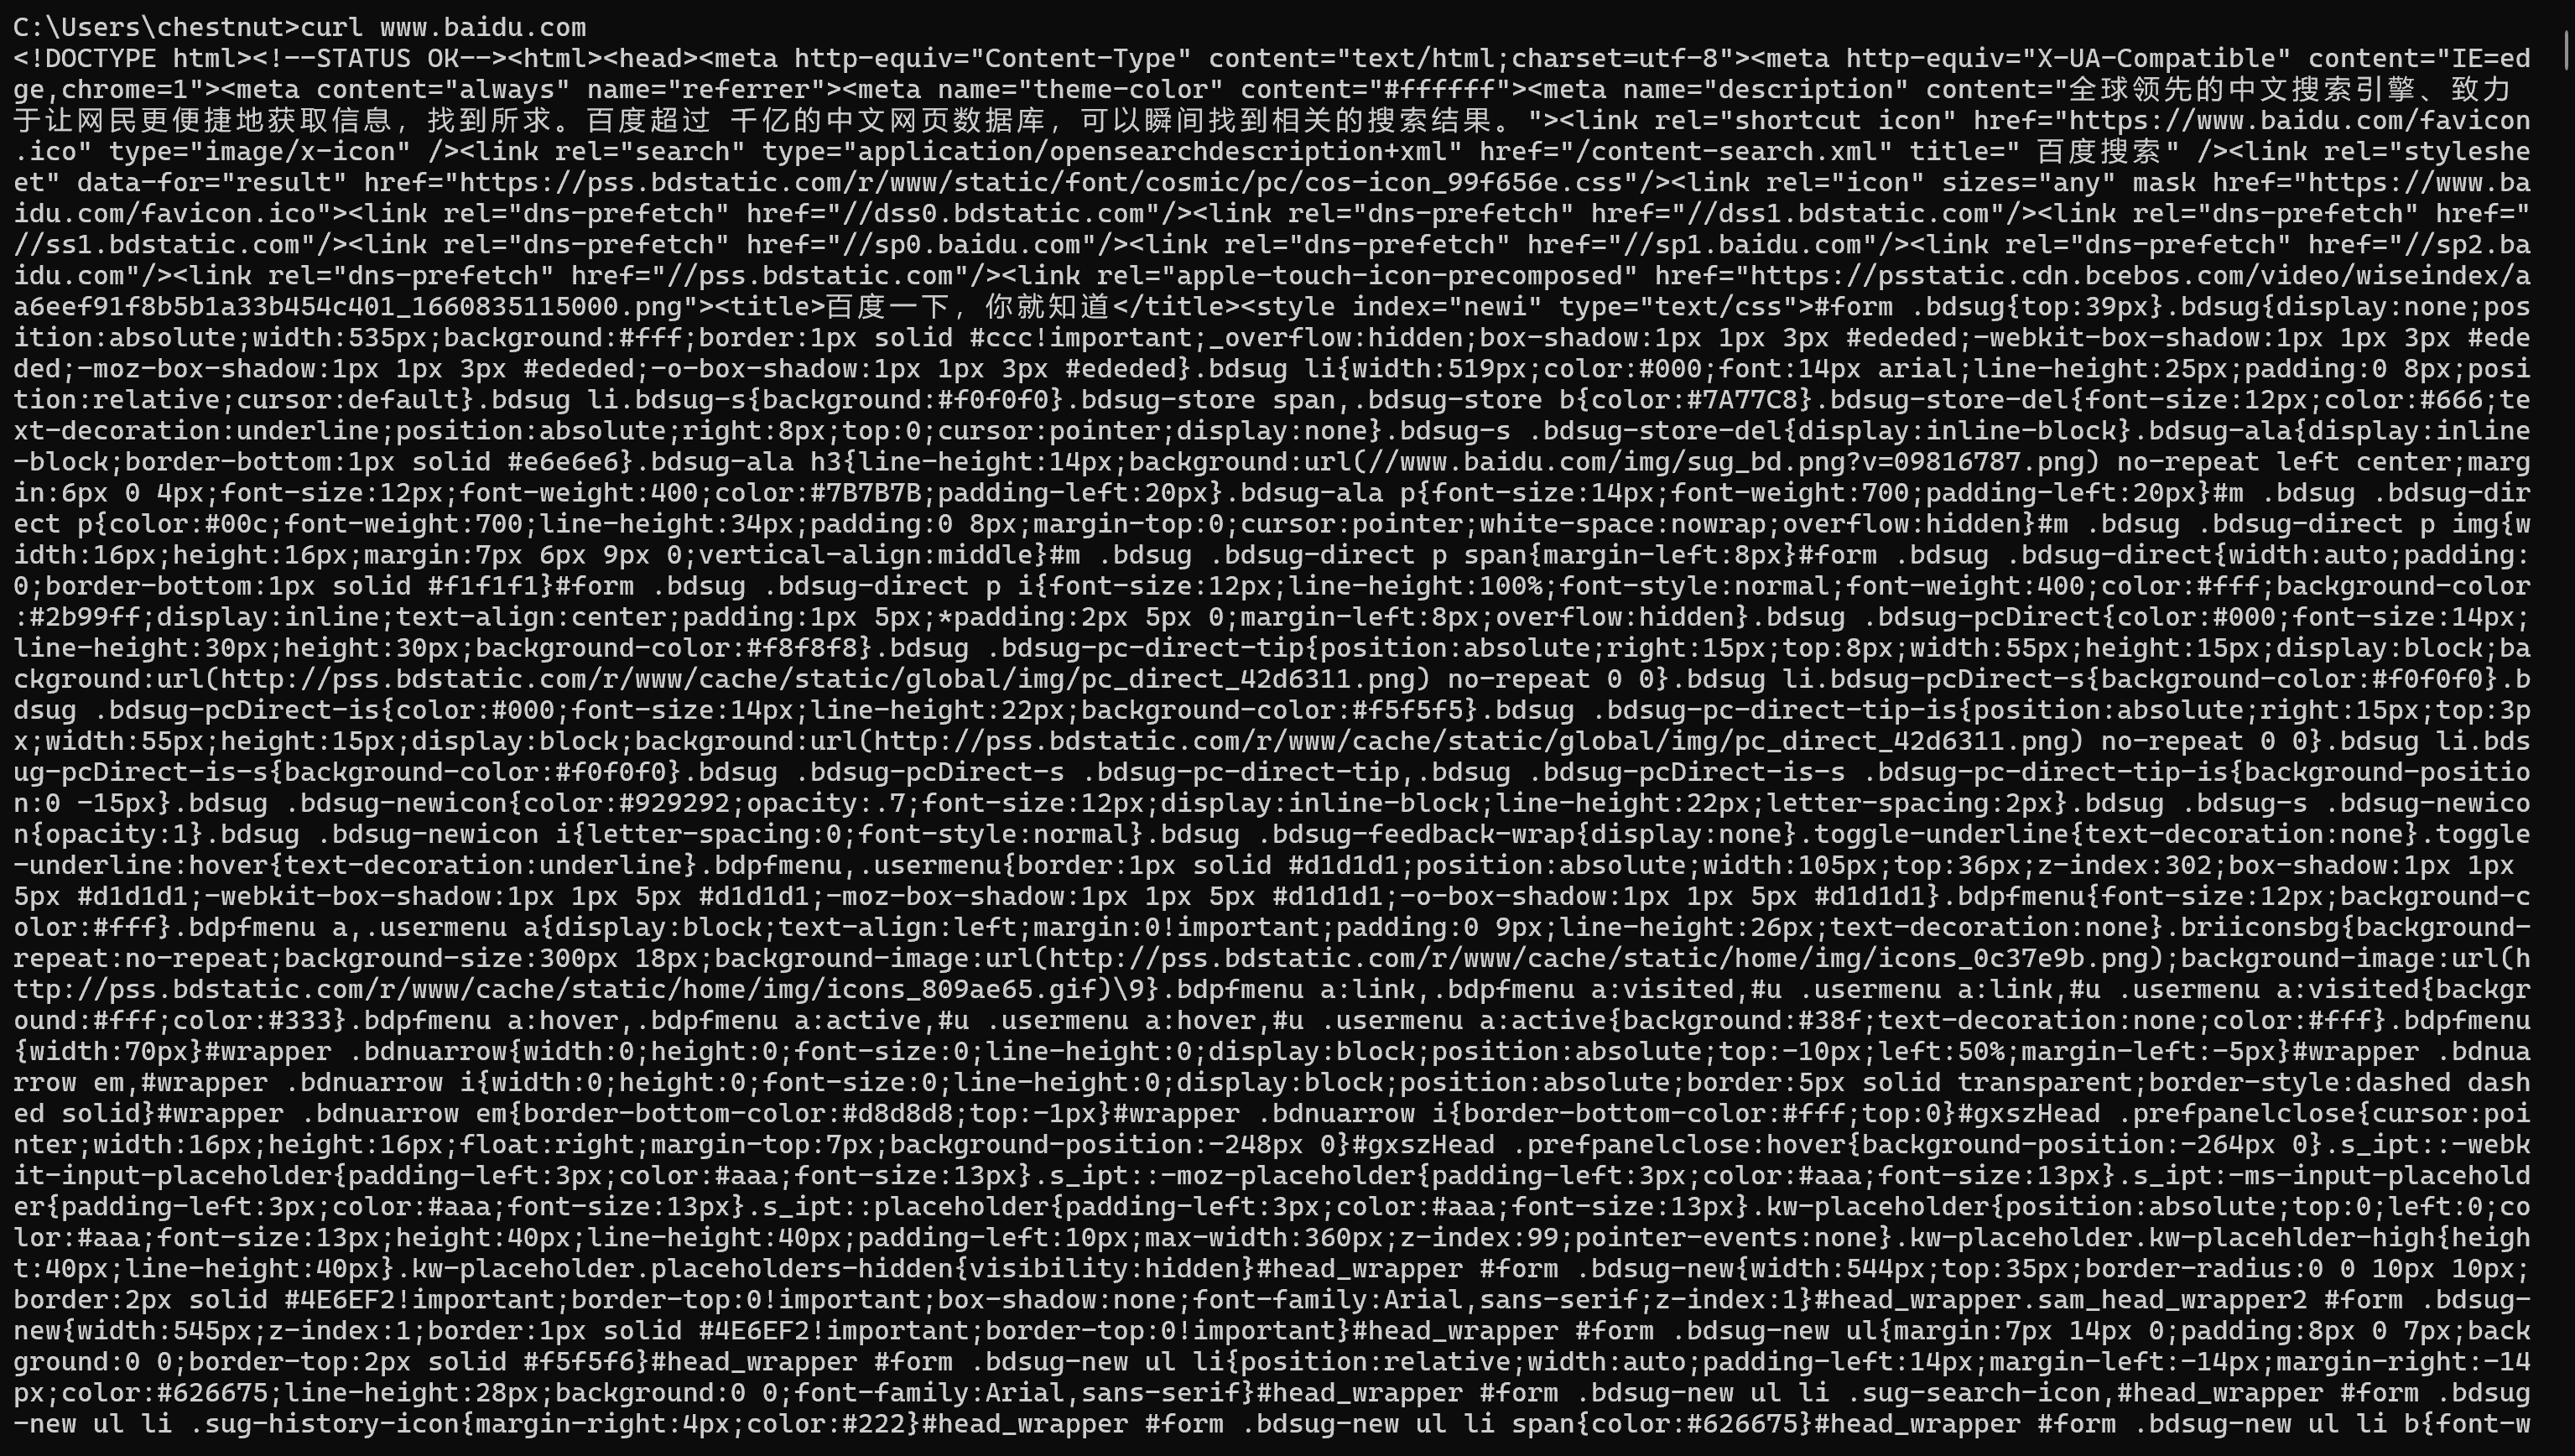
\includegraphics[width=0.8\textwidth]{1_1_images/12.png}}
\vspace{10pt}
返回内容是百度主页的HTML内容,包含网页的资源源代码,请求成功。

\vspace{10pt}
\centerline{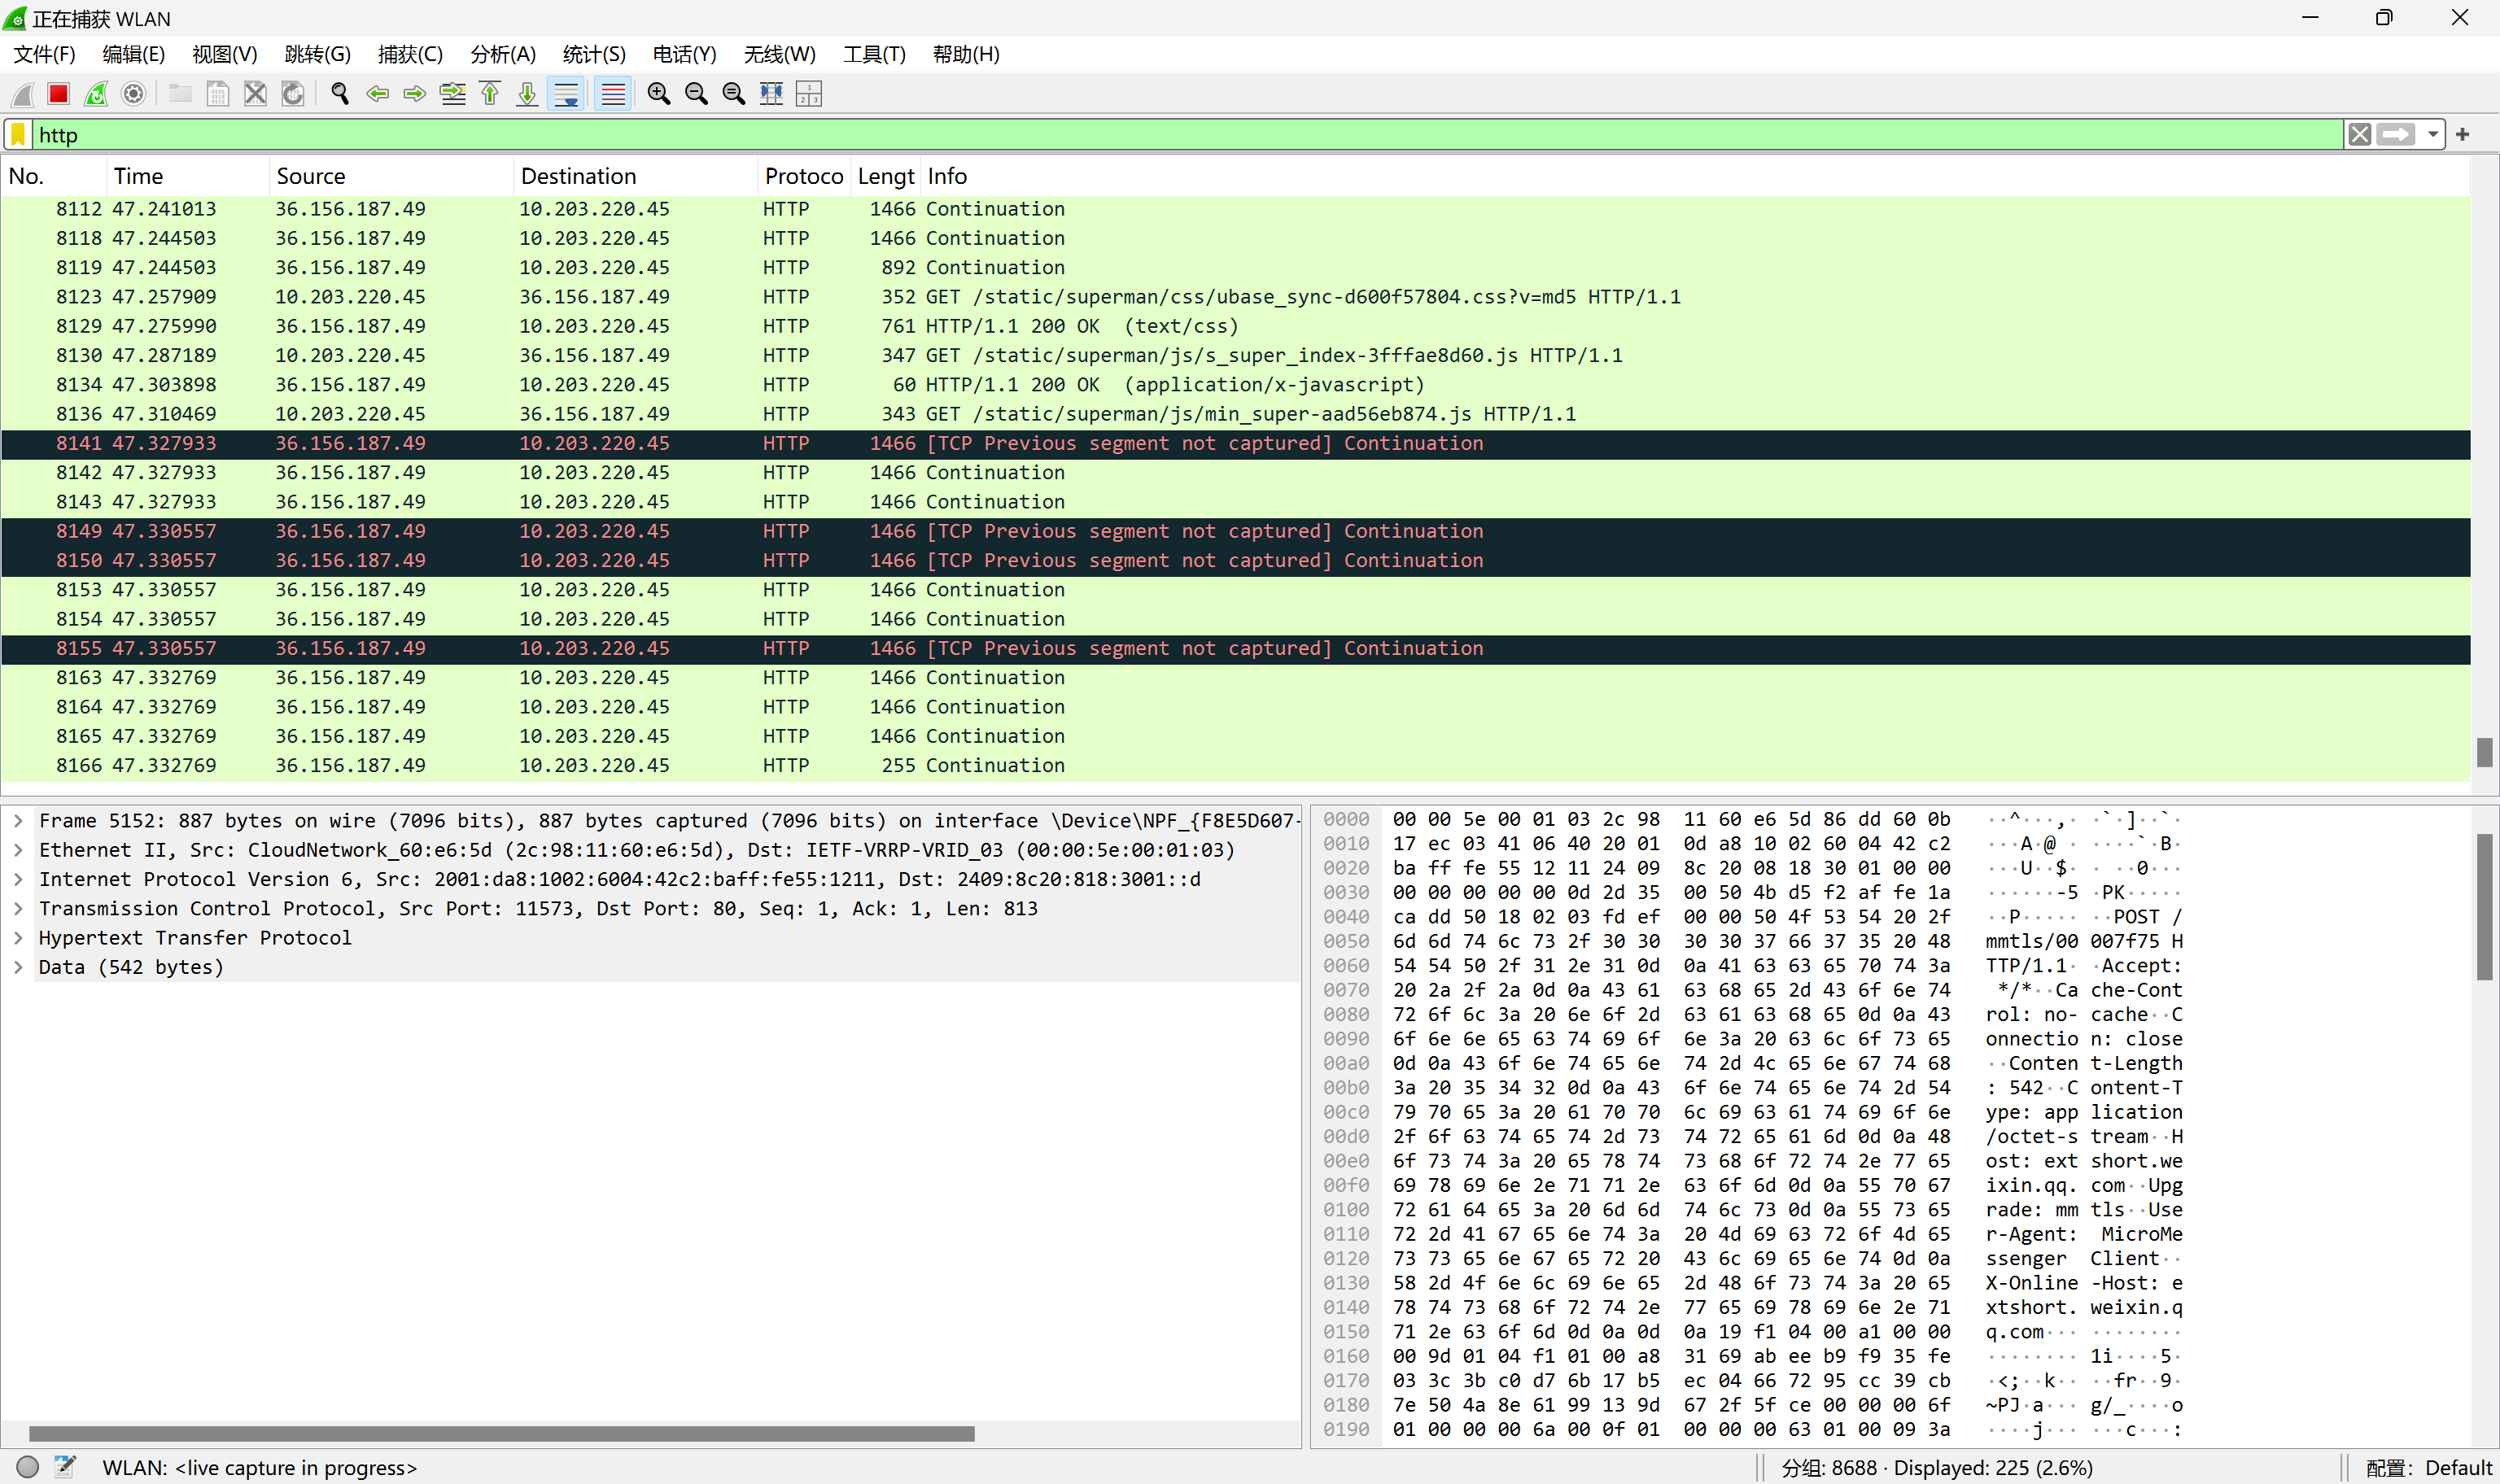
\includegraphics[width=0.8\textwidth]{1_1_images/13.png}}
\vspace{10pt}
在抓包结果中可以看到HTTP的GET请求和服务器返回的状态。36.156.187.49 向 10.203.220.45 发起HTTP请求,在捕获的包中,有多个对静态资源的 GET 请求,HTTP/1.1 200 OK 响应状态显示在第8129和8134行,表示这些资源成功获取并返回。在行号8141至8155间,出现了多次 [TCP Previous segment not captured] 的标记,这说明在抓包过程中可能存在丢包,导致TCP连接中的某些段没有被捕获。

\subsubsection{利用telnet命令测试get命令,访问www.baidu.com。}
首先在命令行中输入telnet www.baidu.com 80连接到百度的80端口,然后输入GET / HTTP/1.1		Host: www.baidu.com发送HTTP GET请求,然后能看到百度返回的响应数据: 

\vspace{10pt}
\centerline{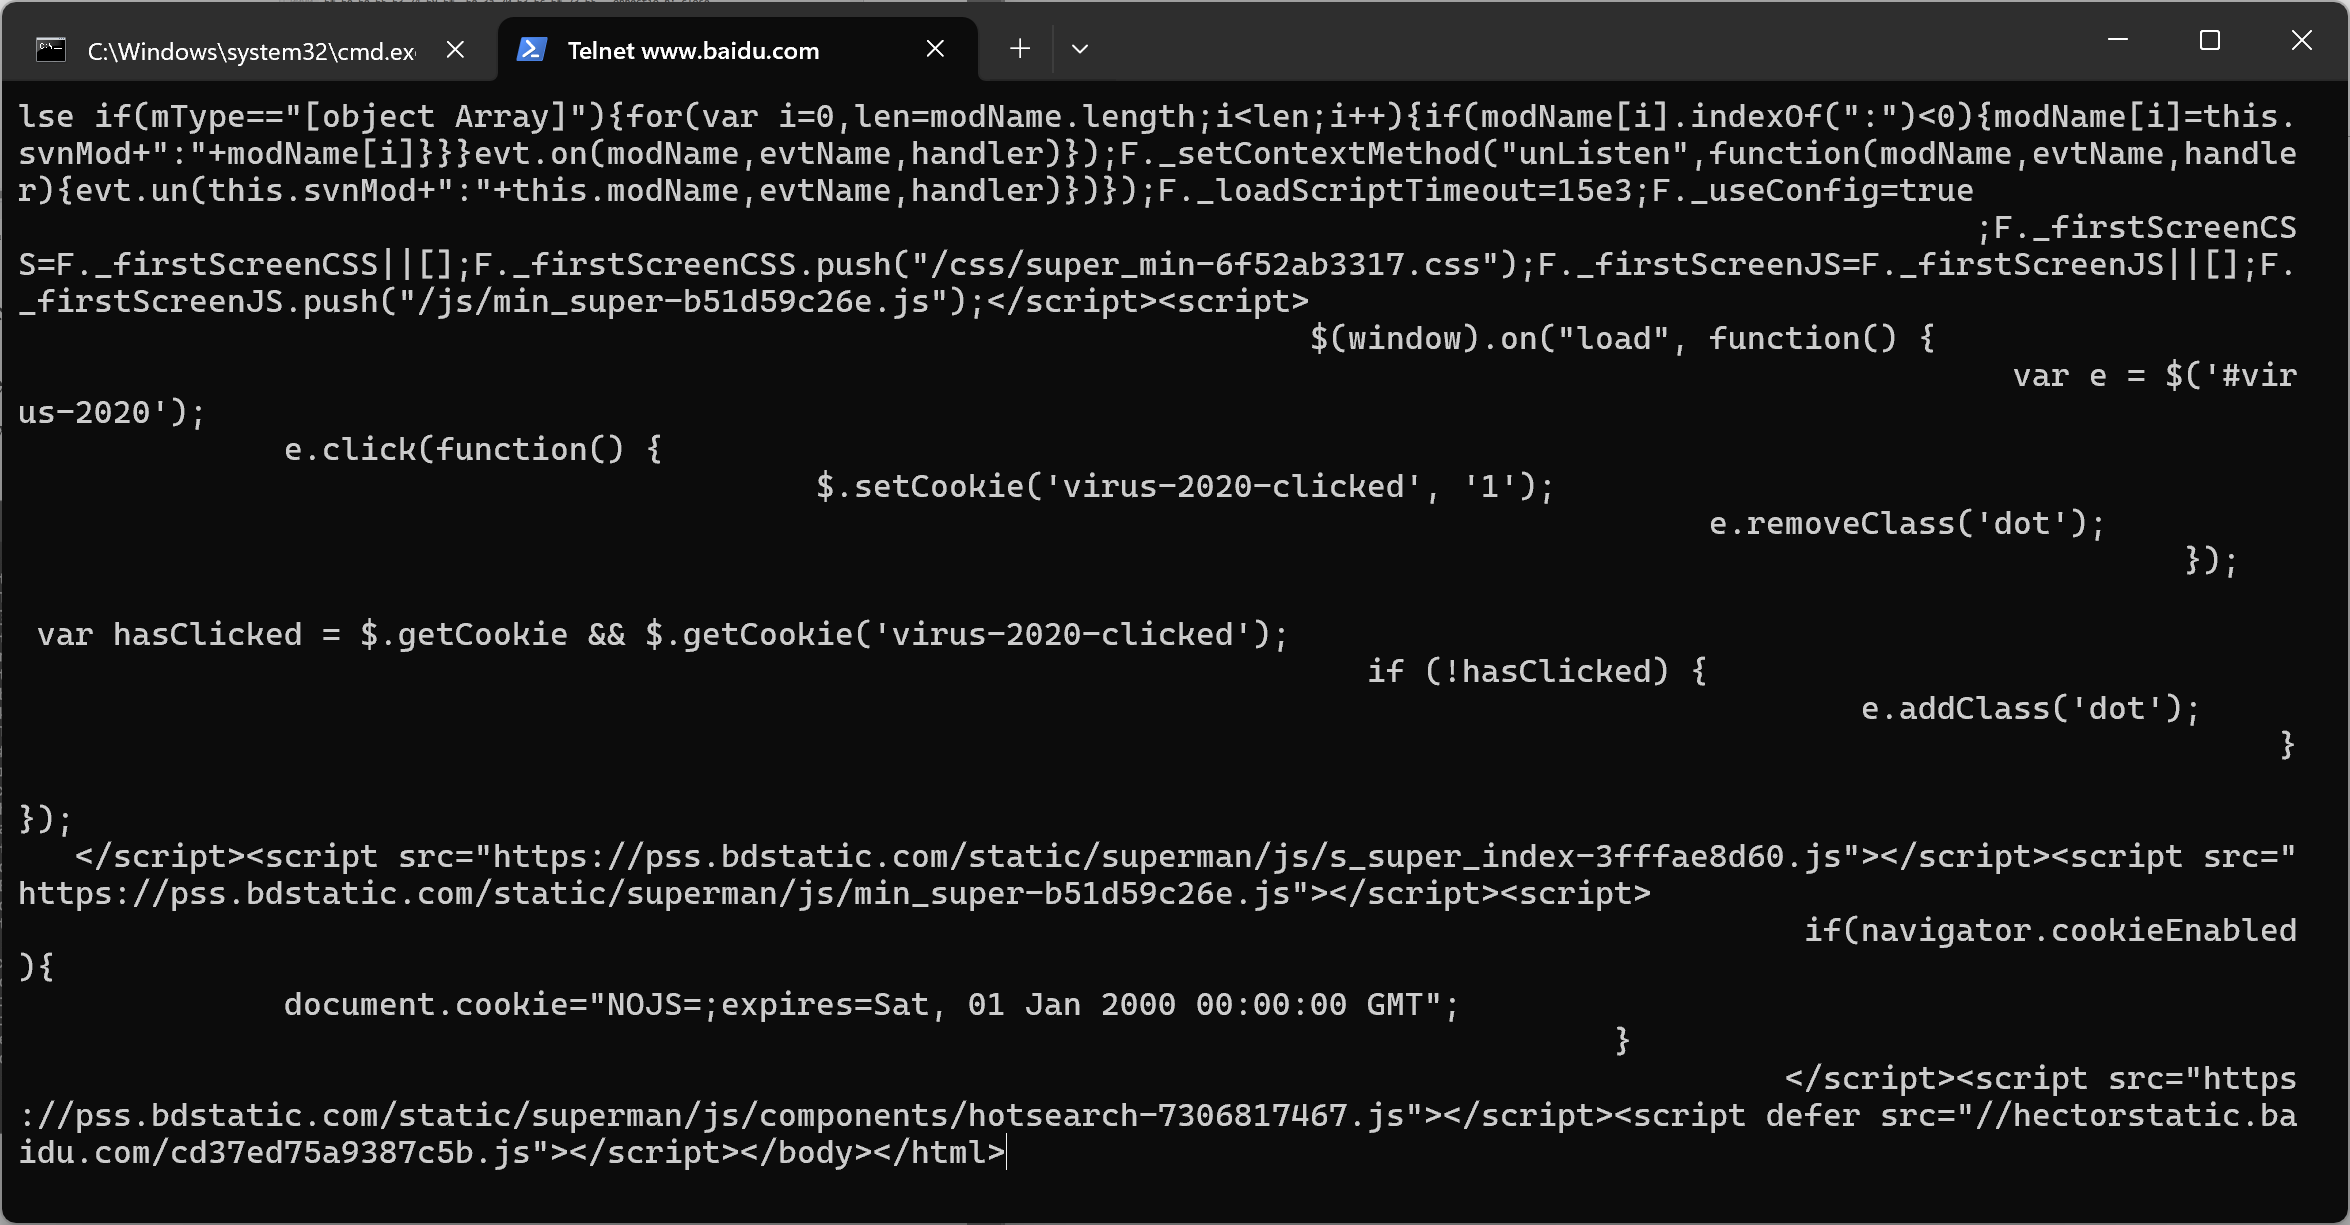
\includegraphics[width=0.8\textwidth]{1_1_images/14.png}}
\vspace{10pt}
抓包情况如下:

\vspace{10pt}
\centerline{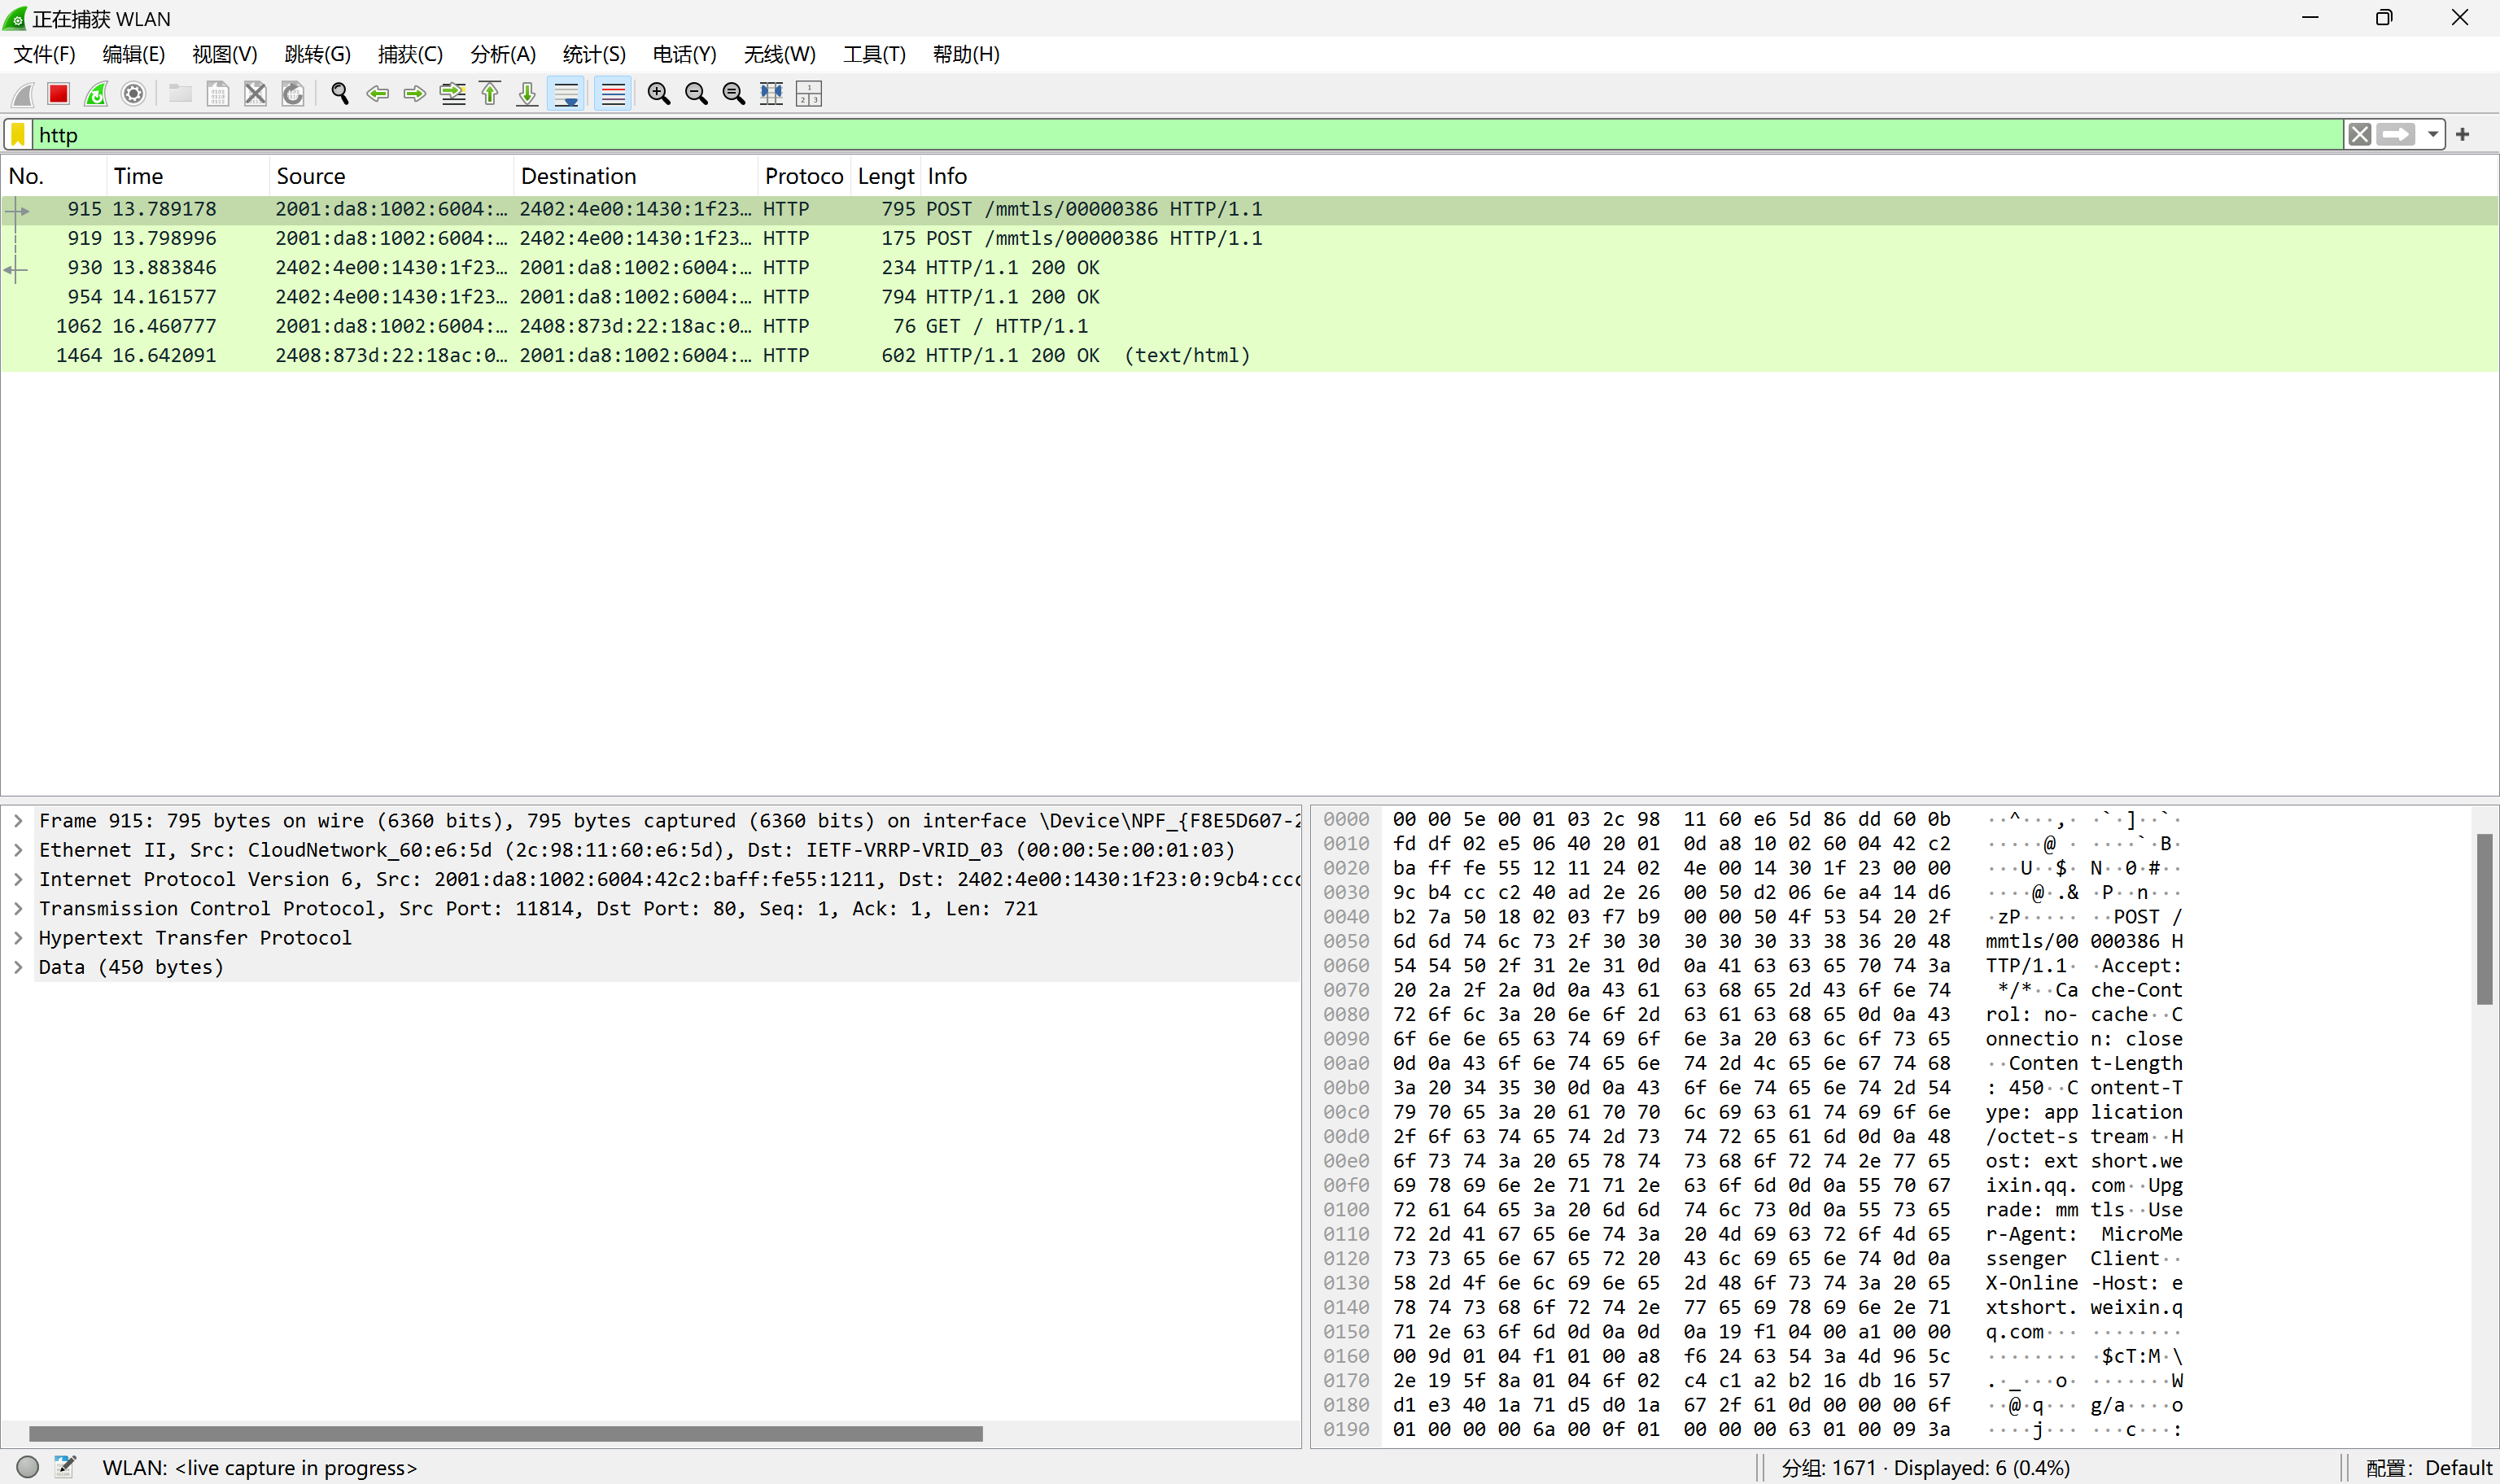
\includegraphics[width=0.8\textwidth]{1_1_images/15.png}}
\vspace{10pt}
结果显示收到一个GET和POST请求,对POST请求的响应状态码是 HTTP/1.1 200 OK,说明服务器成功处理了这些请求,给予了响应。

\subsubsection{利用telnet命令测试SMTP服务,解析其过程。}
在命令输入:
\begin{lstlisting}
telnet smtp.163.com 25
helo 163.com
auth login
mail_base64
pass_base64
mail from: <XXX.com>
rcpt to: <XXX.com>
data
subject: test by telnet
mail test
.
Quit
\end{lstlisting}
由于qq授权码的问题连接账户失败:

\vspace{10pt}
\centerline{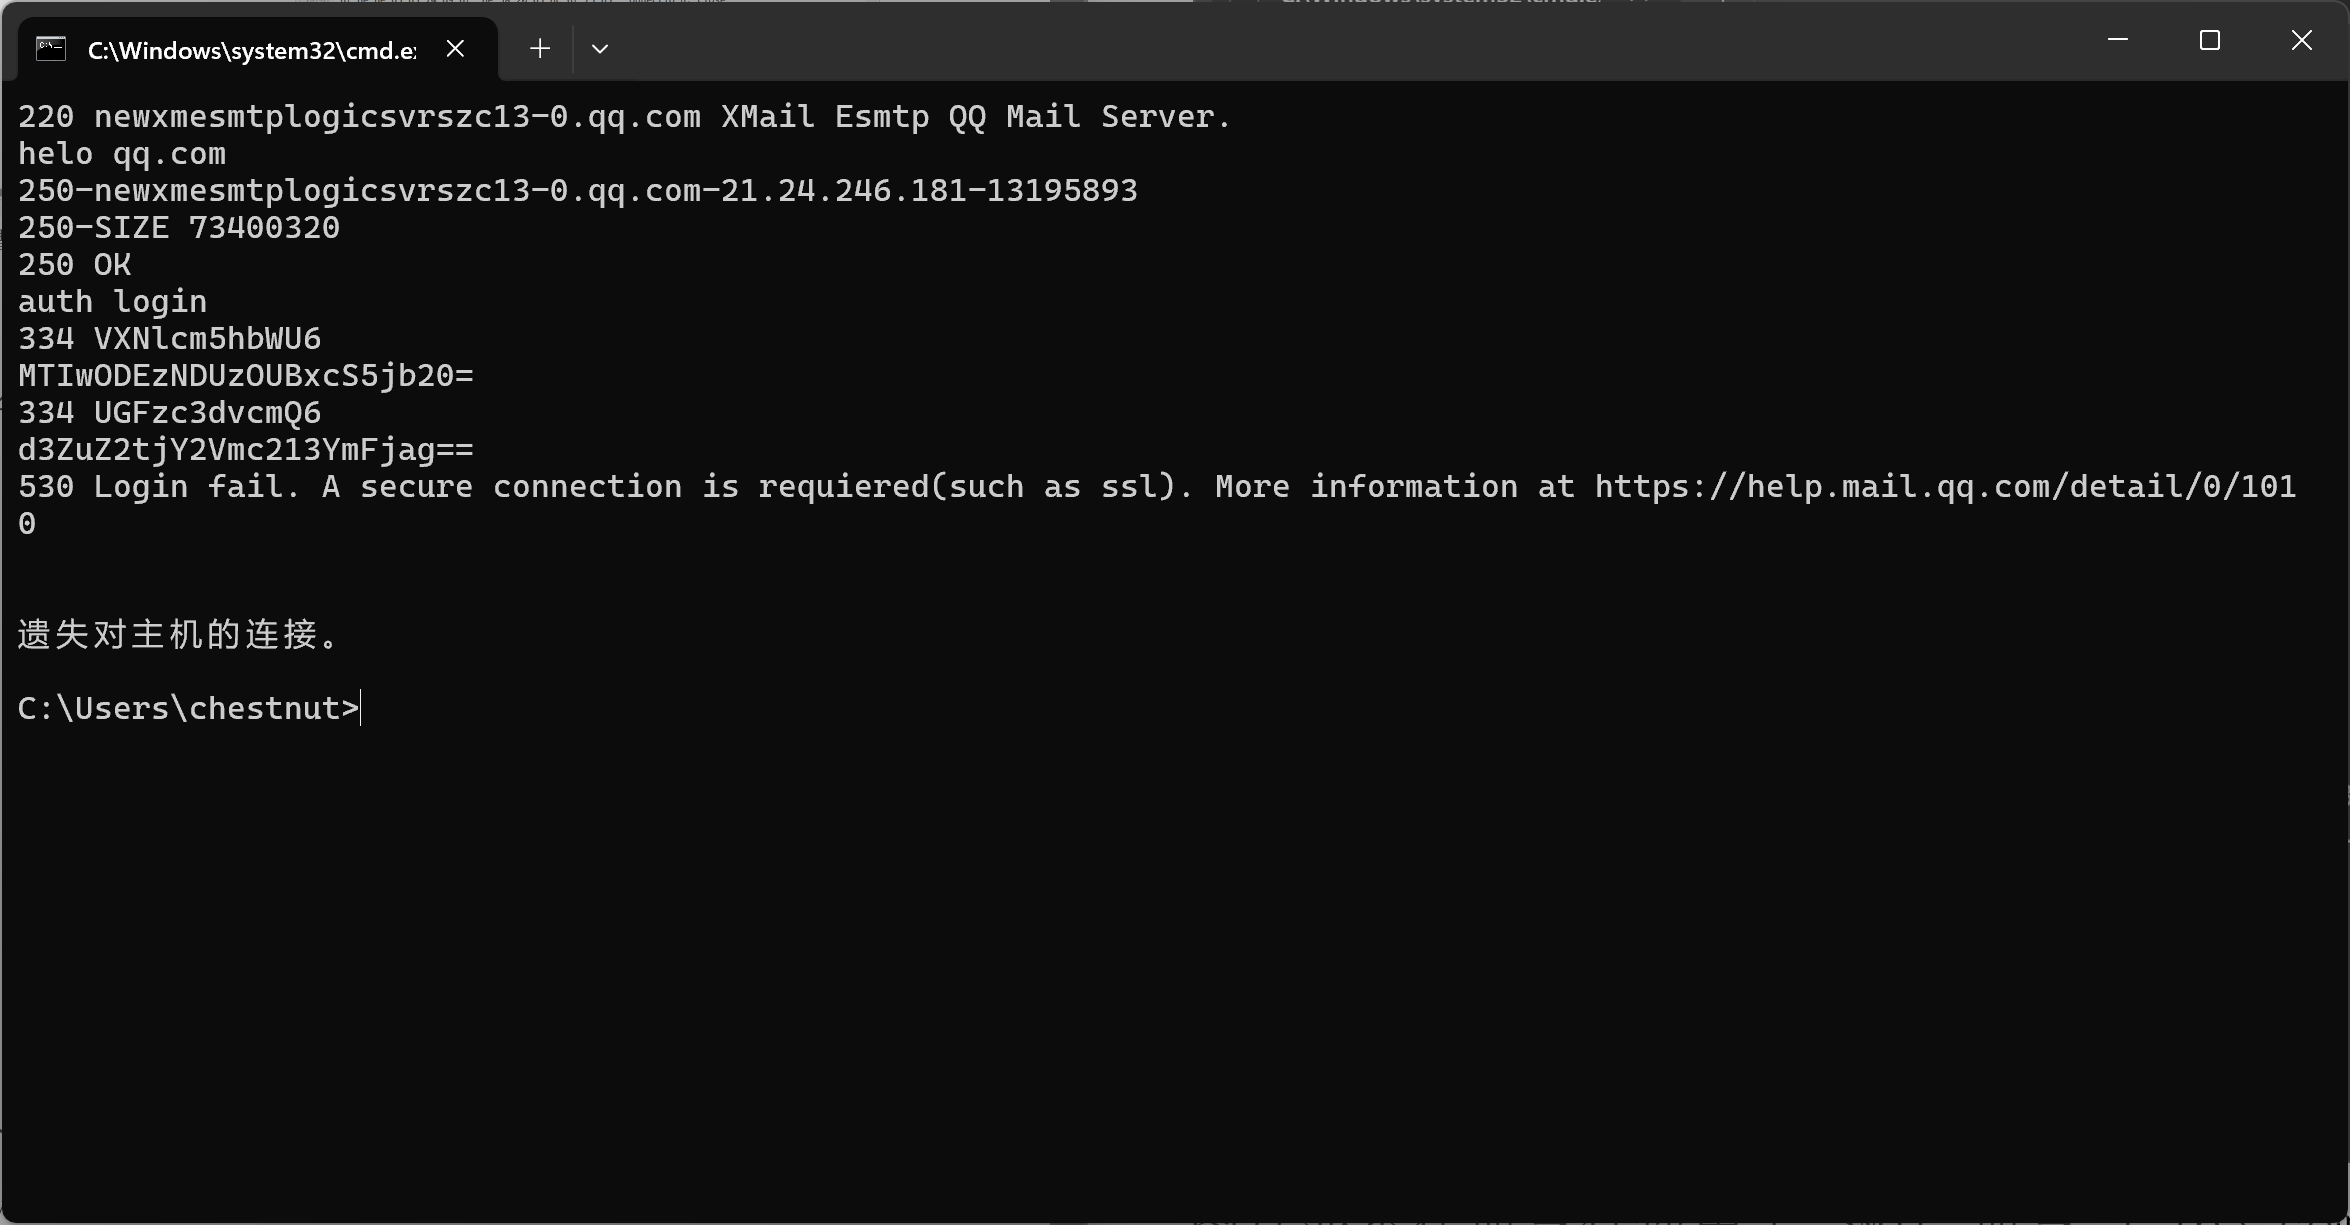
\includegraphics[width=0.8\textwidth]{1_1_images/16.png}}
\vspace{10pt}
此时抓包情况如下:

\vspace{10pt}
\centerline{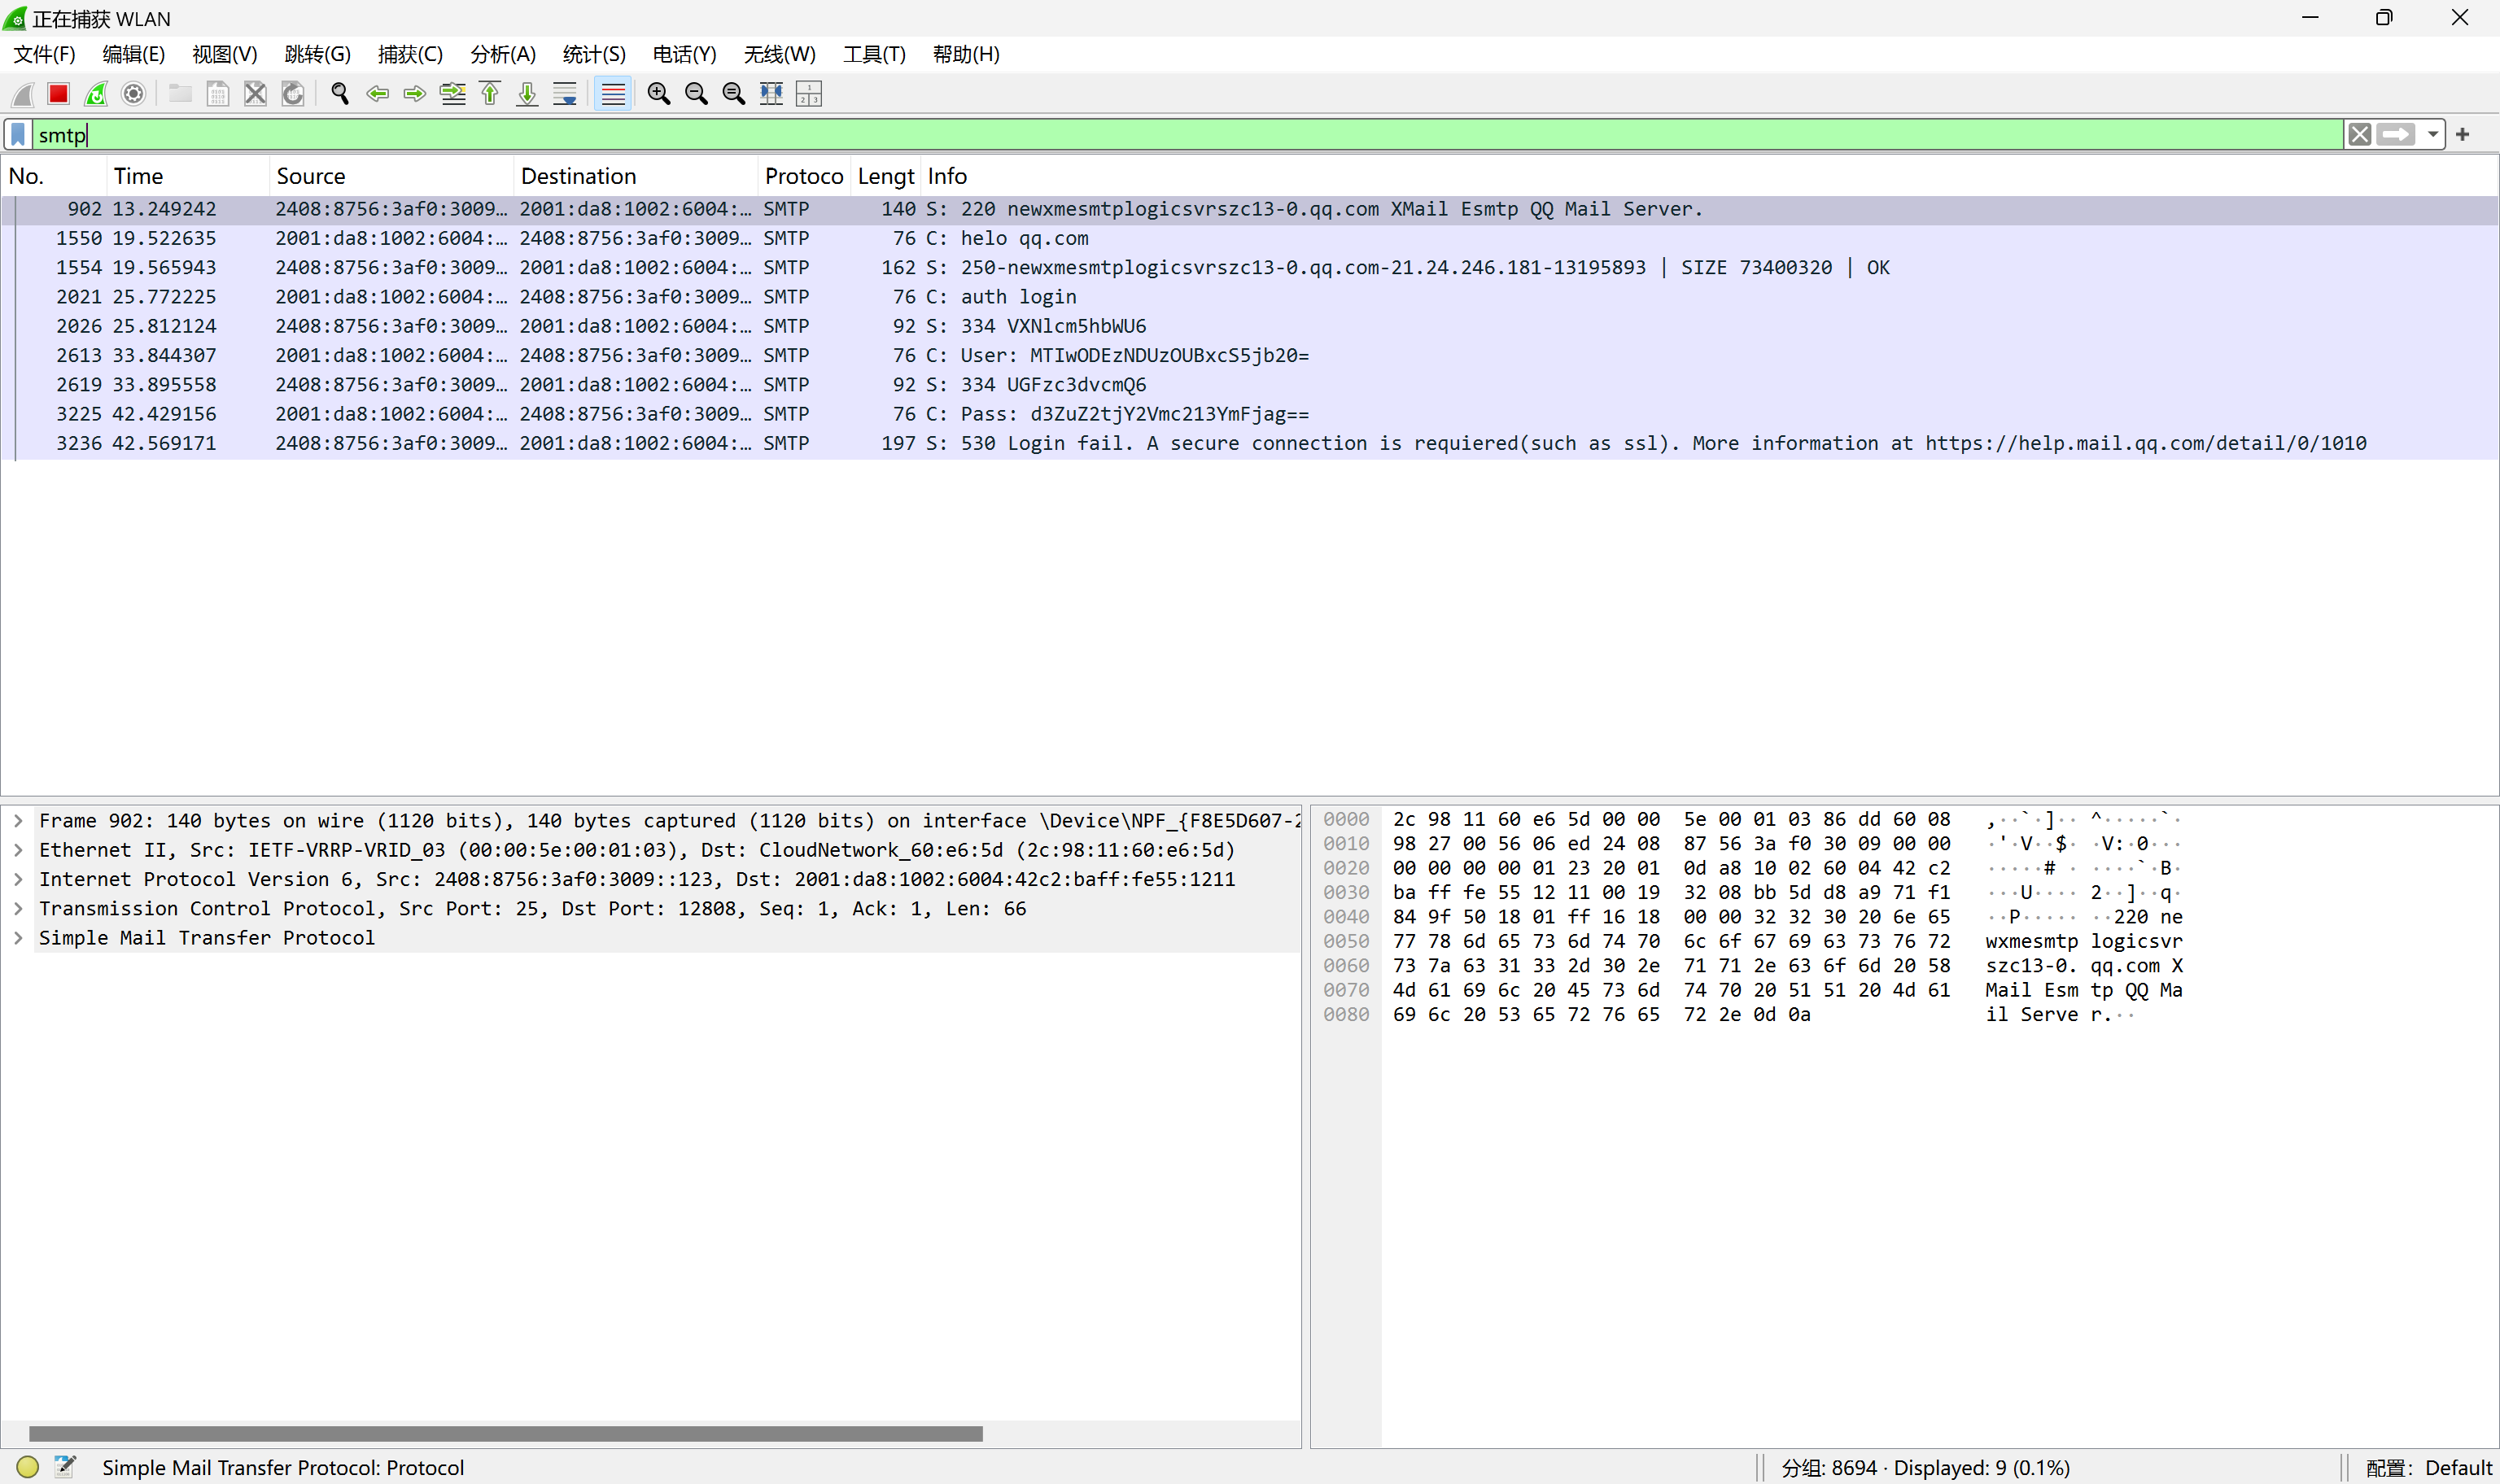
\includegraphics[width=0.8\textwidth]{1_1_images/17.png}}
\vspace{10pt}
显示客户端成功连接到了 qq.com 的 SMTP 服务器,收到服务器的欢迎信息,状态码为 220,显示服务器名称 newxmesmtplogicsvrszc13-0.qq.com。
客户端发送了 HELO qq.com,服务器返回 250 状态码作为回应,表示 HELO 命令成功,并提供服务器信息。
客户端发送 AUTH LOGIN 命令,要求进行登录认证。
服务器返回 334 状态码,表示它准备接受用户名。
显示服务器返回 530 状态码,并带有错误信息 Login fail.Asecure connection is required(such as ssl) ...表示登录失败,因为SMTP服务器要求使用SSL加密连接来保护登录信息。

\subsubsection{测试tracert命令,并解析其过程。}
在命令行进行tracert www.baidu.com的操作:

\vspace{10pt}
\centerline{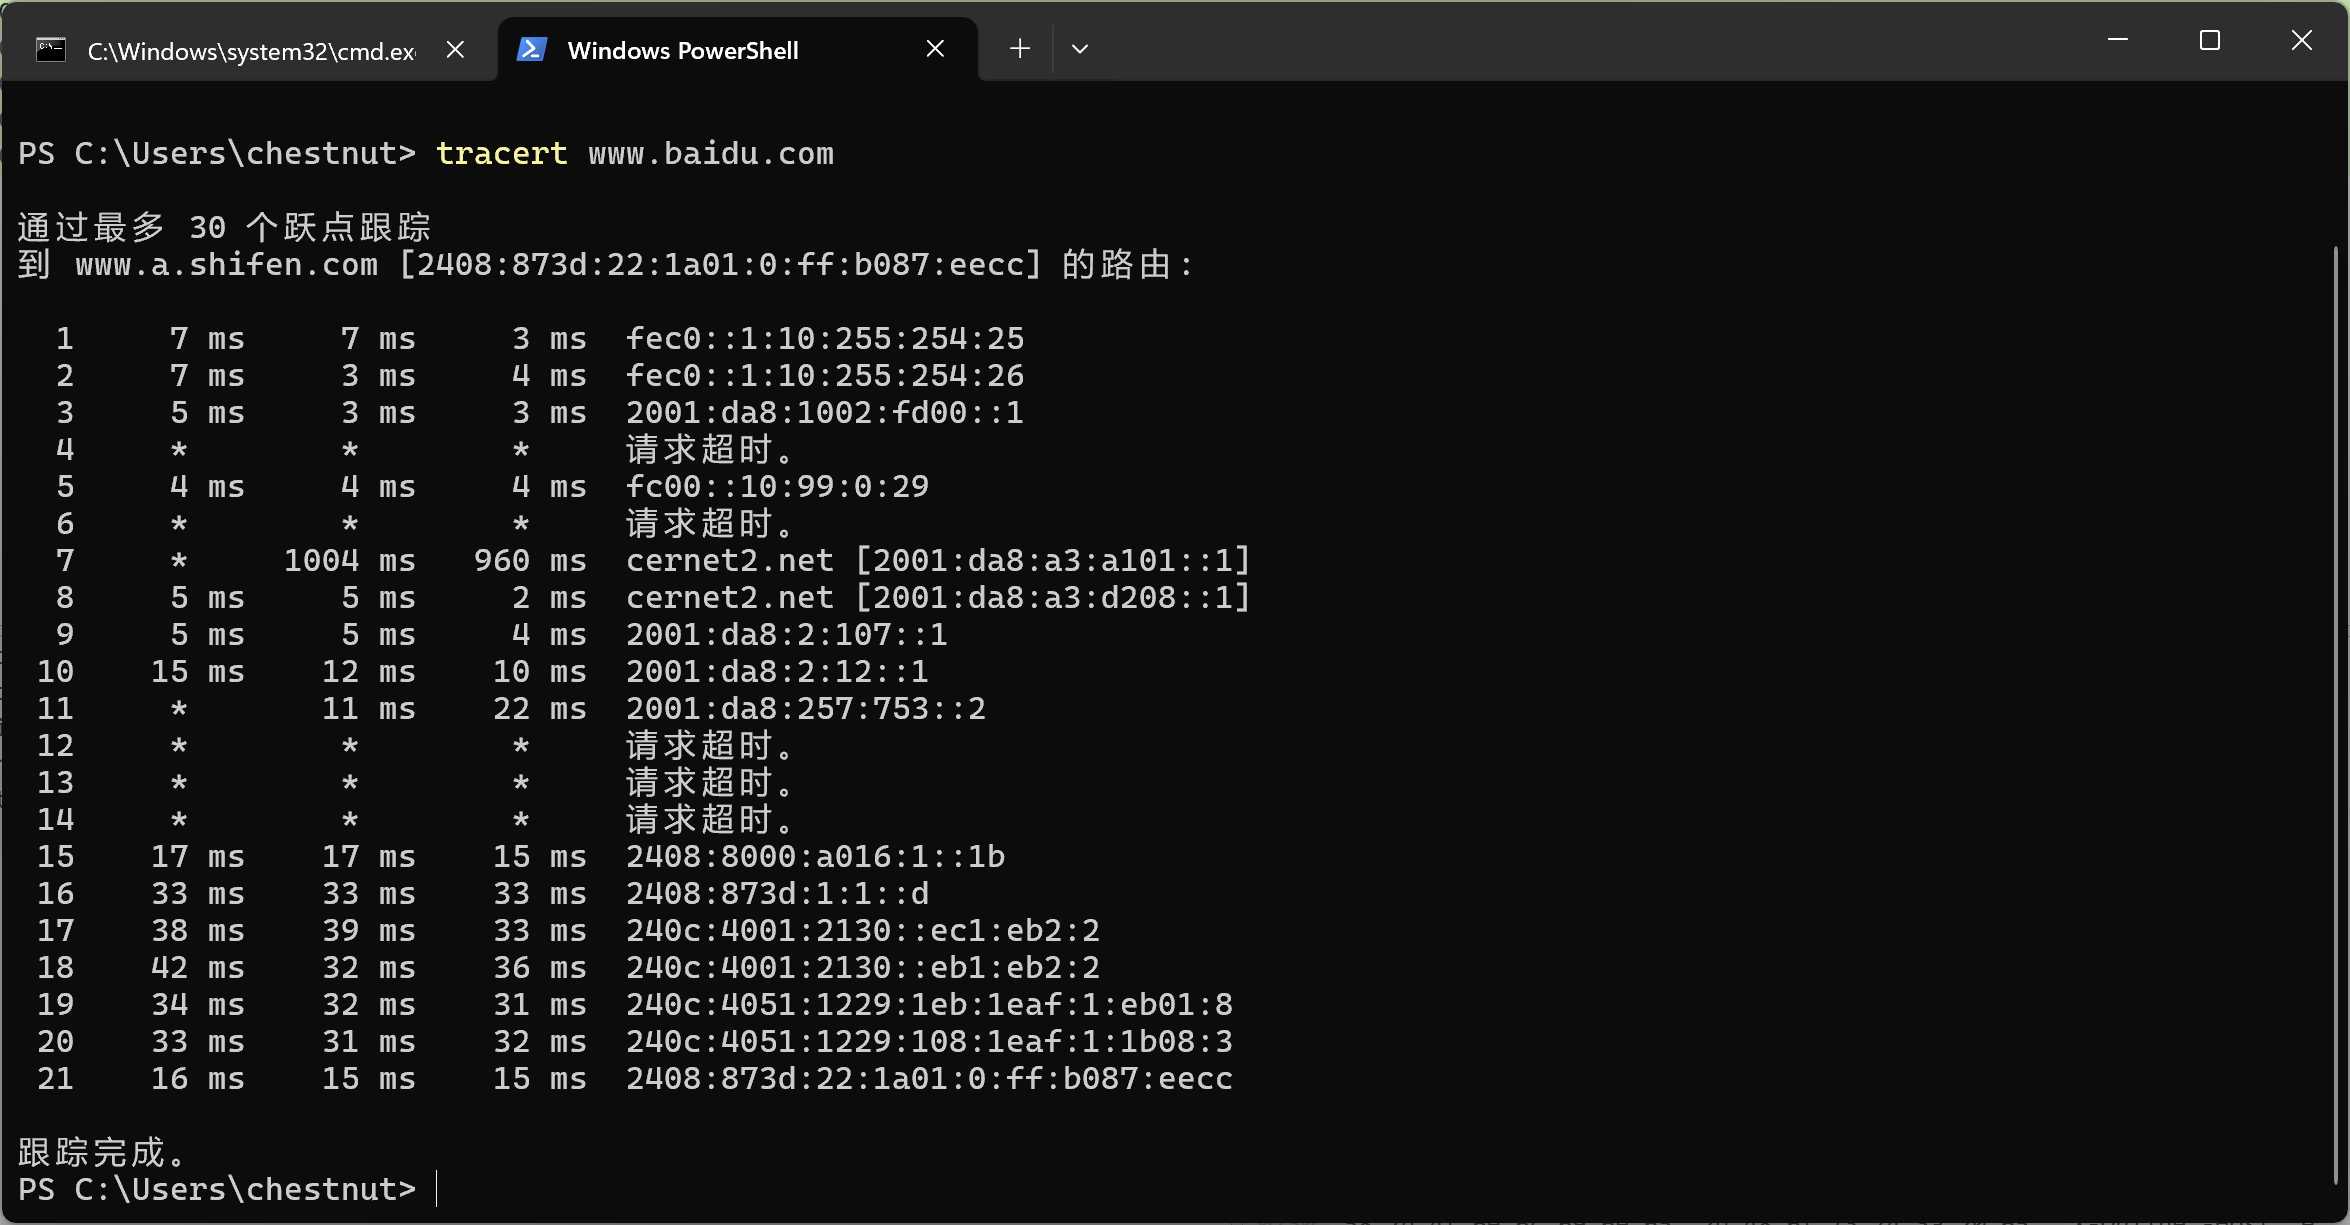
\includegraphics[width=0.8\textwidth]{1_1_images/18.png}}
\vspace{10pt}
显示追踪百度网站经历的网络结点,一共21个跃点,在4,12,13,14跃点有丢包,其他网络连接都比较好。
抓包情况如下:

\vspace{10pt}
\centerline{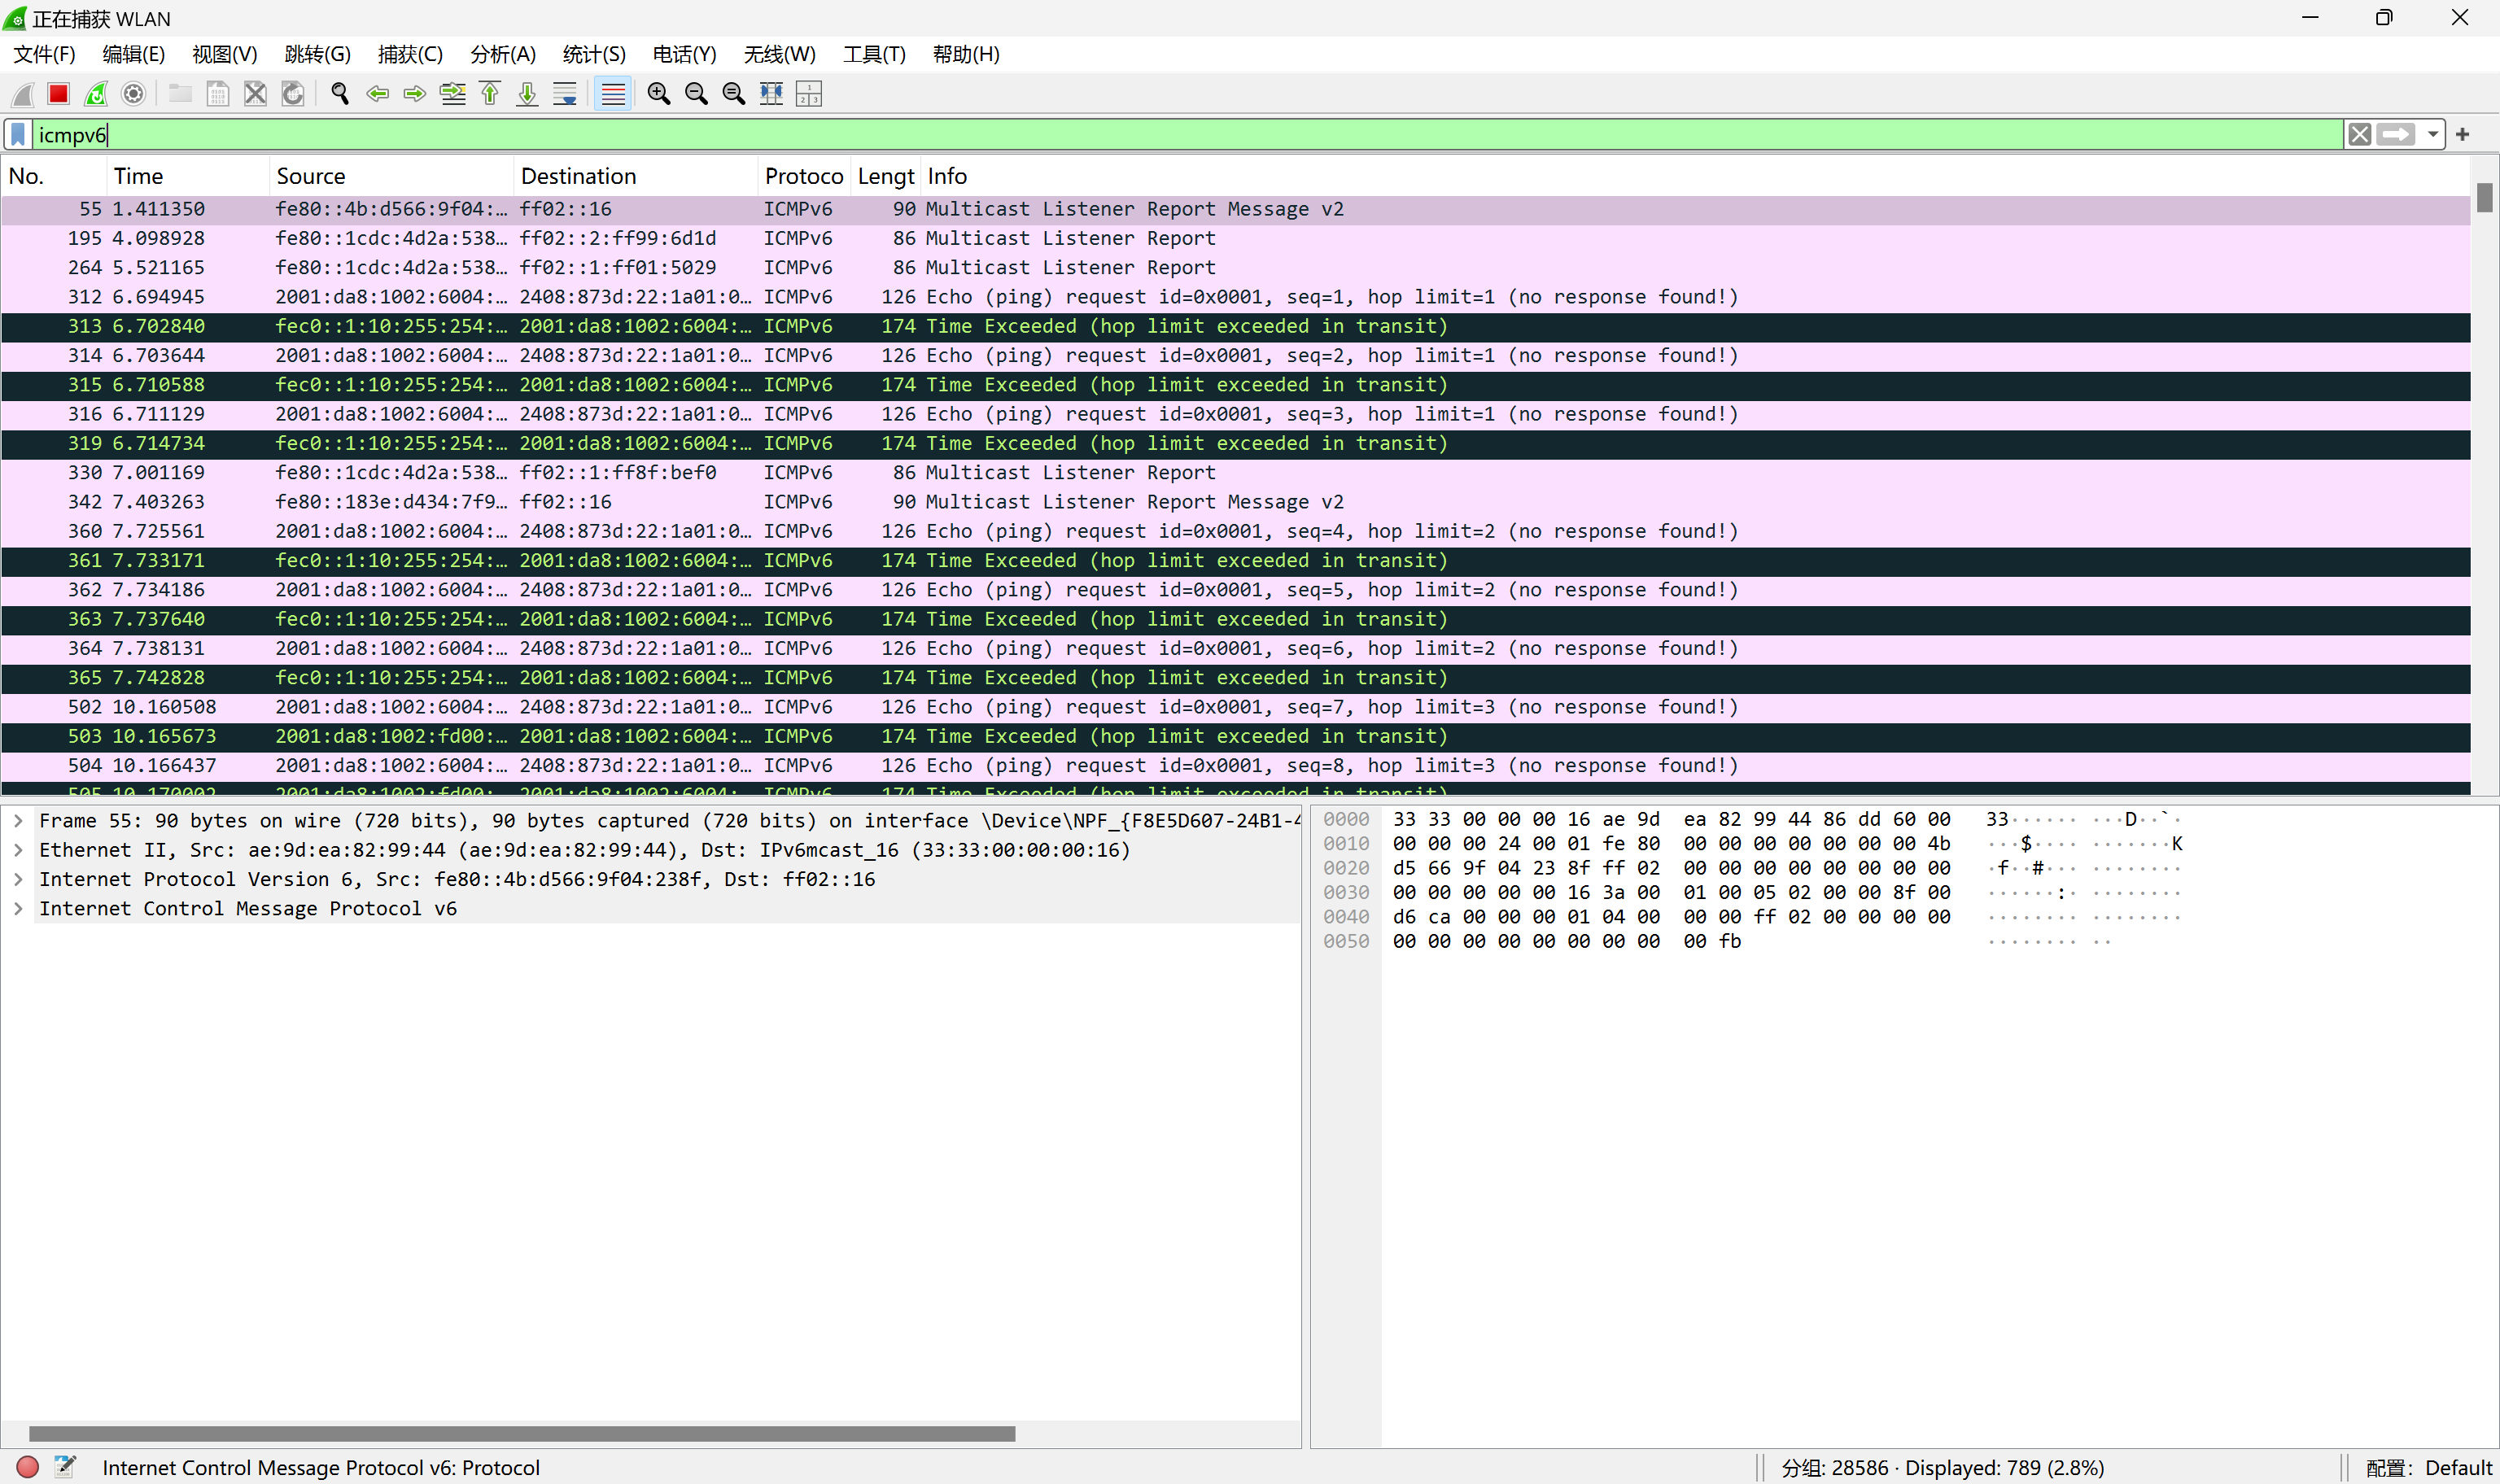
\includegraphics[width=0.8\textwidth]{1_1_images/19.png}}
\vspace{10pt}

Time exceeded表示请求超时,但是大部分都是成功连接的。
\subsubsection{使用nslookup查询域名信息,简要分析。}
在命令行进行nslookup www.baidu.com的操作:

\vspace{10pt}
\centerline{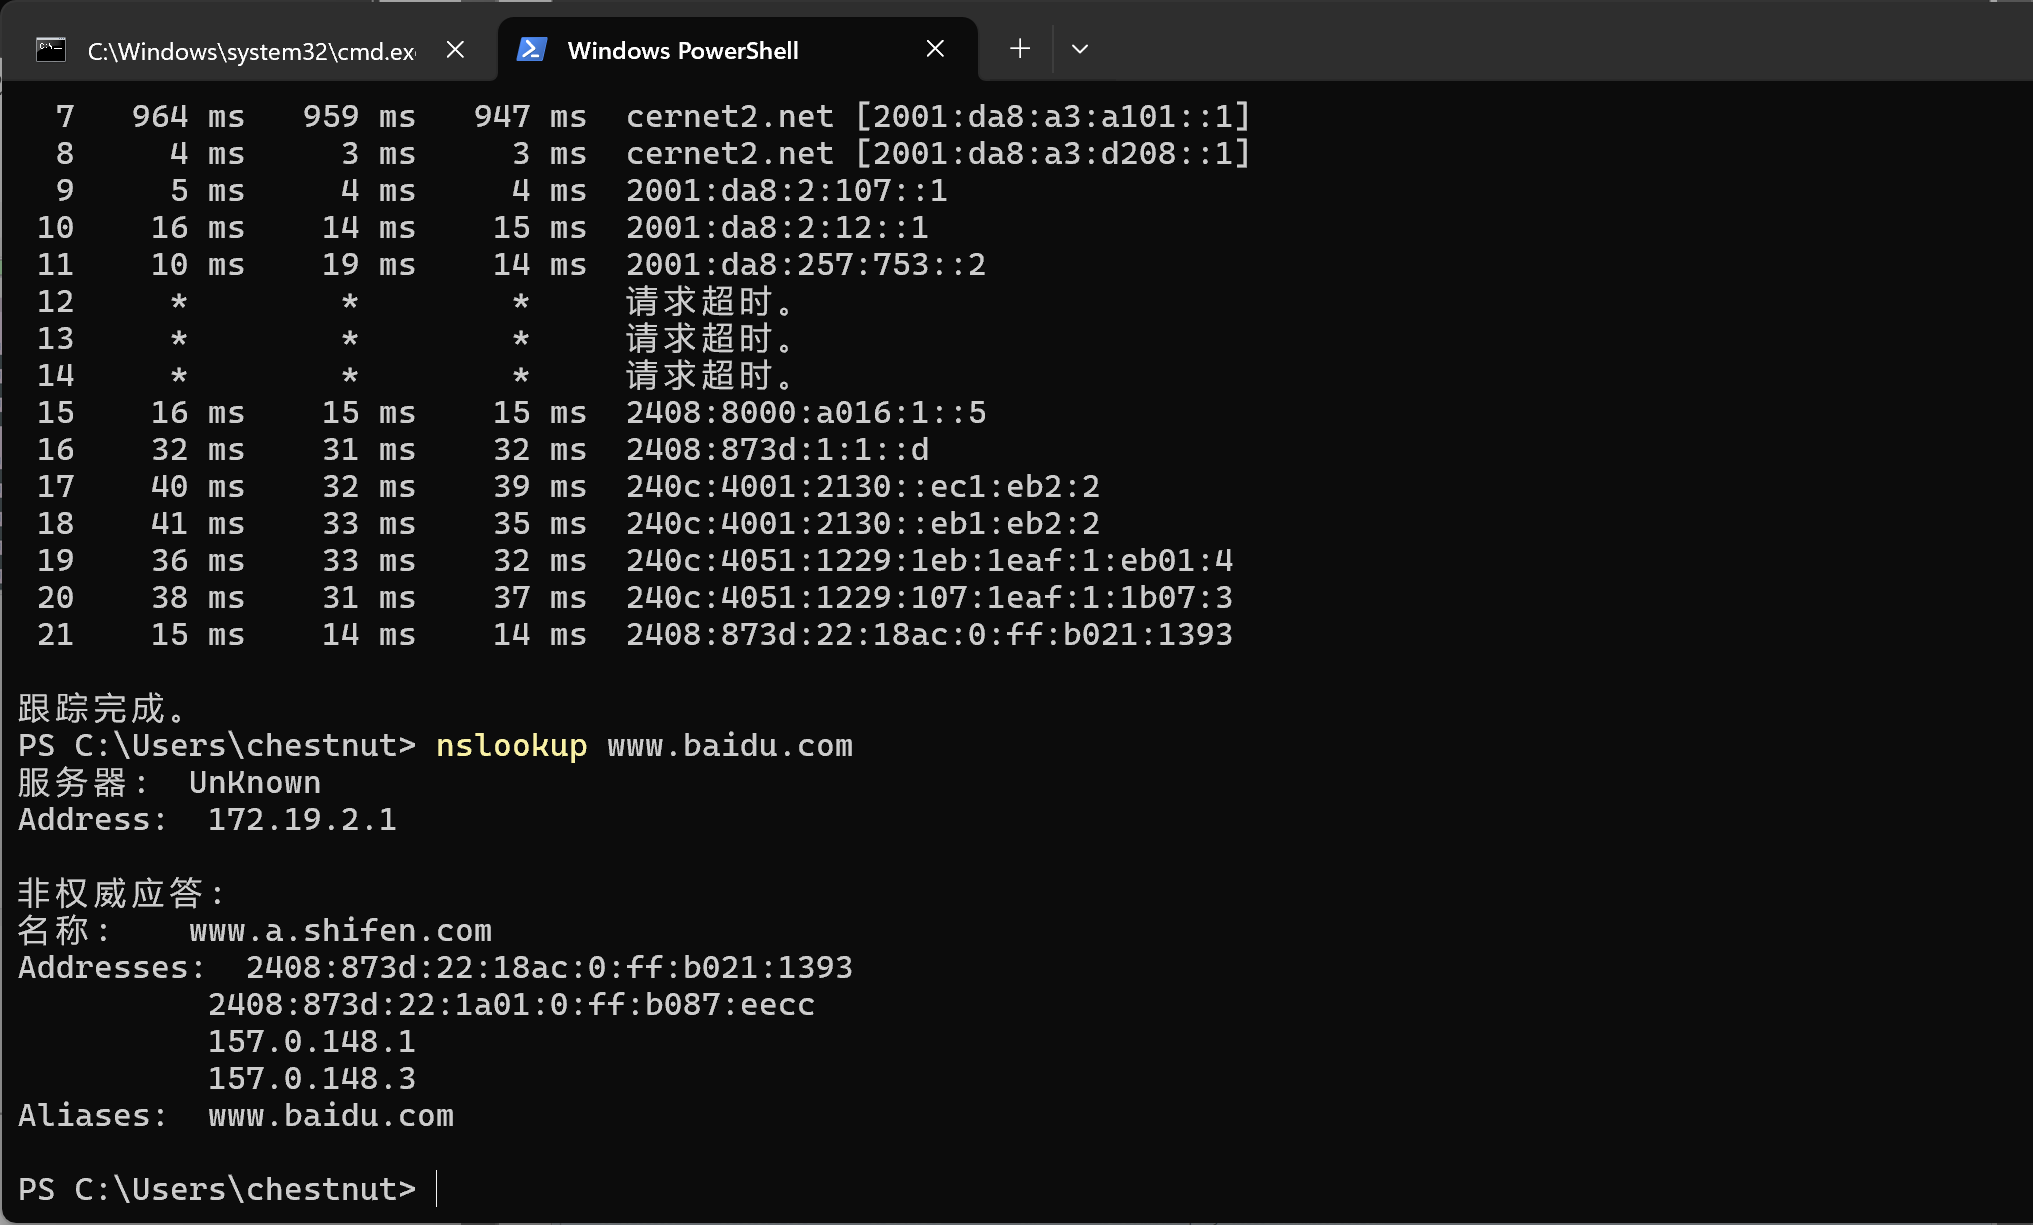
\includegraphics[width=0.8\textwidth]{1_1_images/20.png}}
\vspace{10pt}
抓包信息如下:

\vspace{10pt}
\centerline{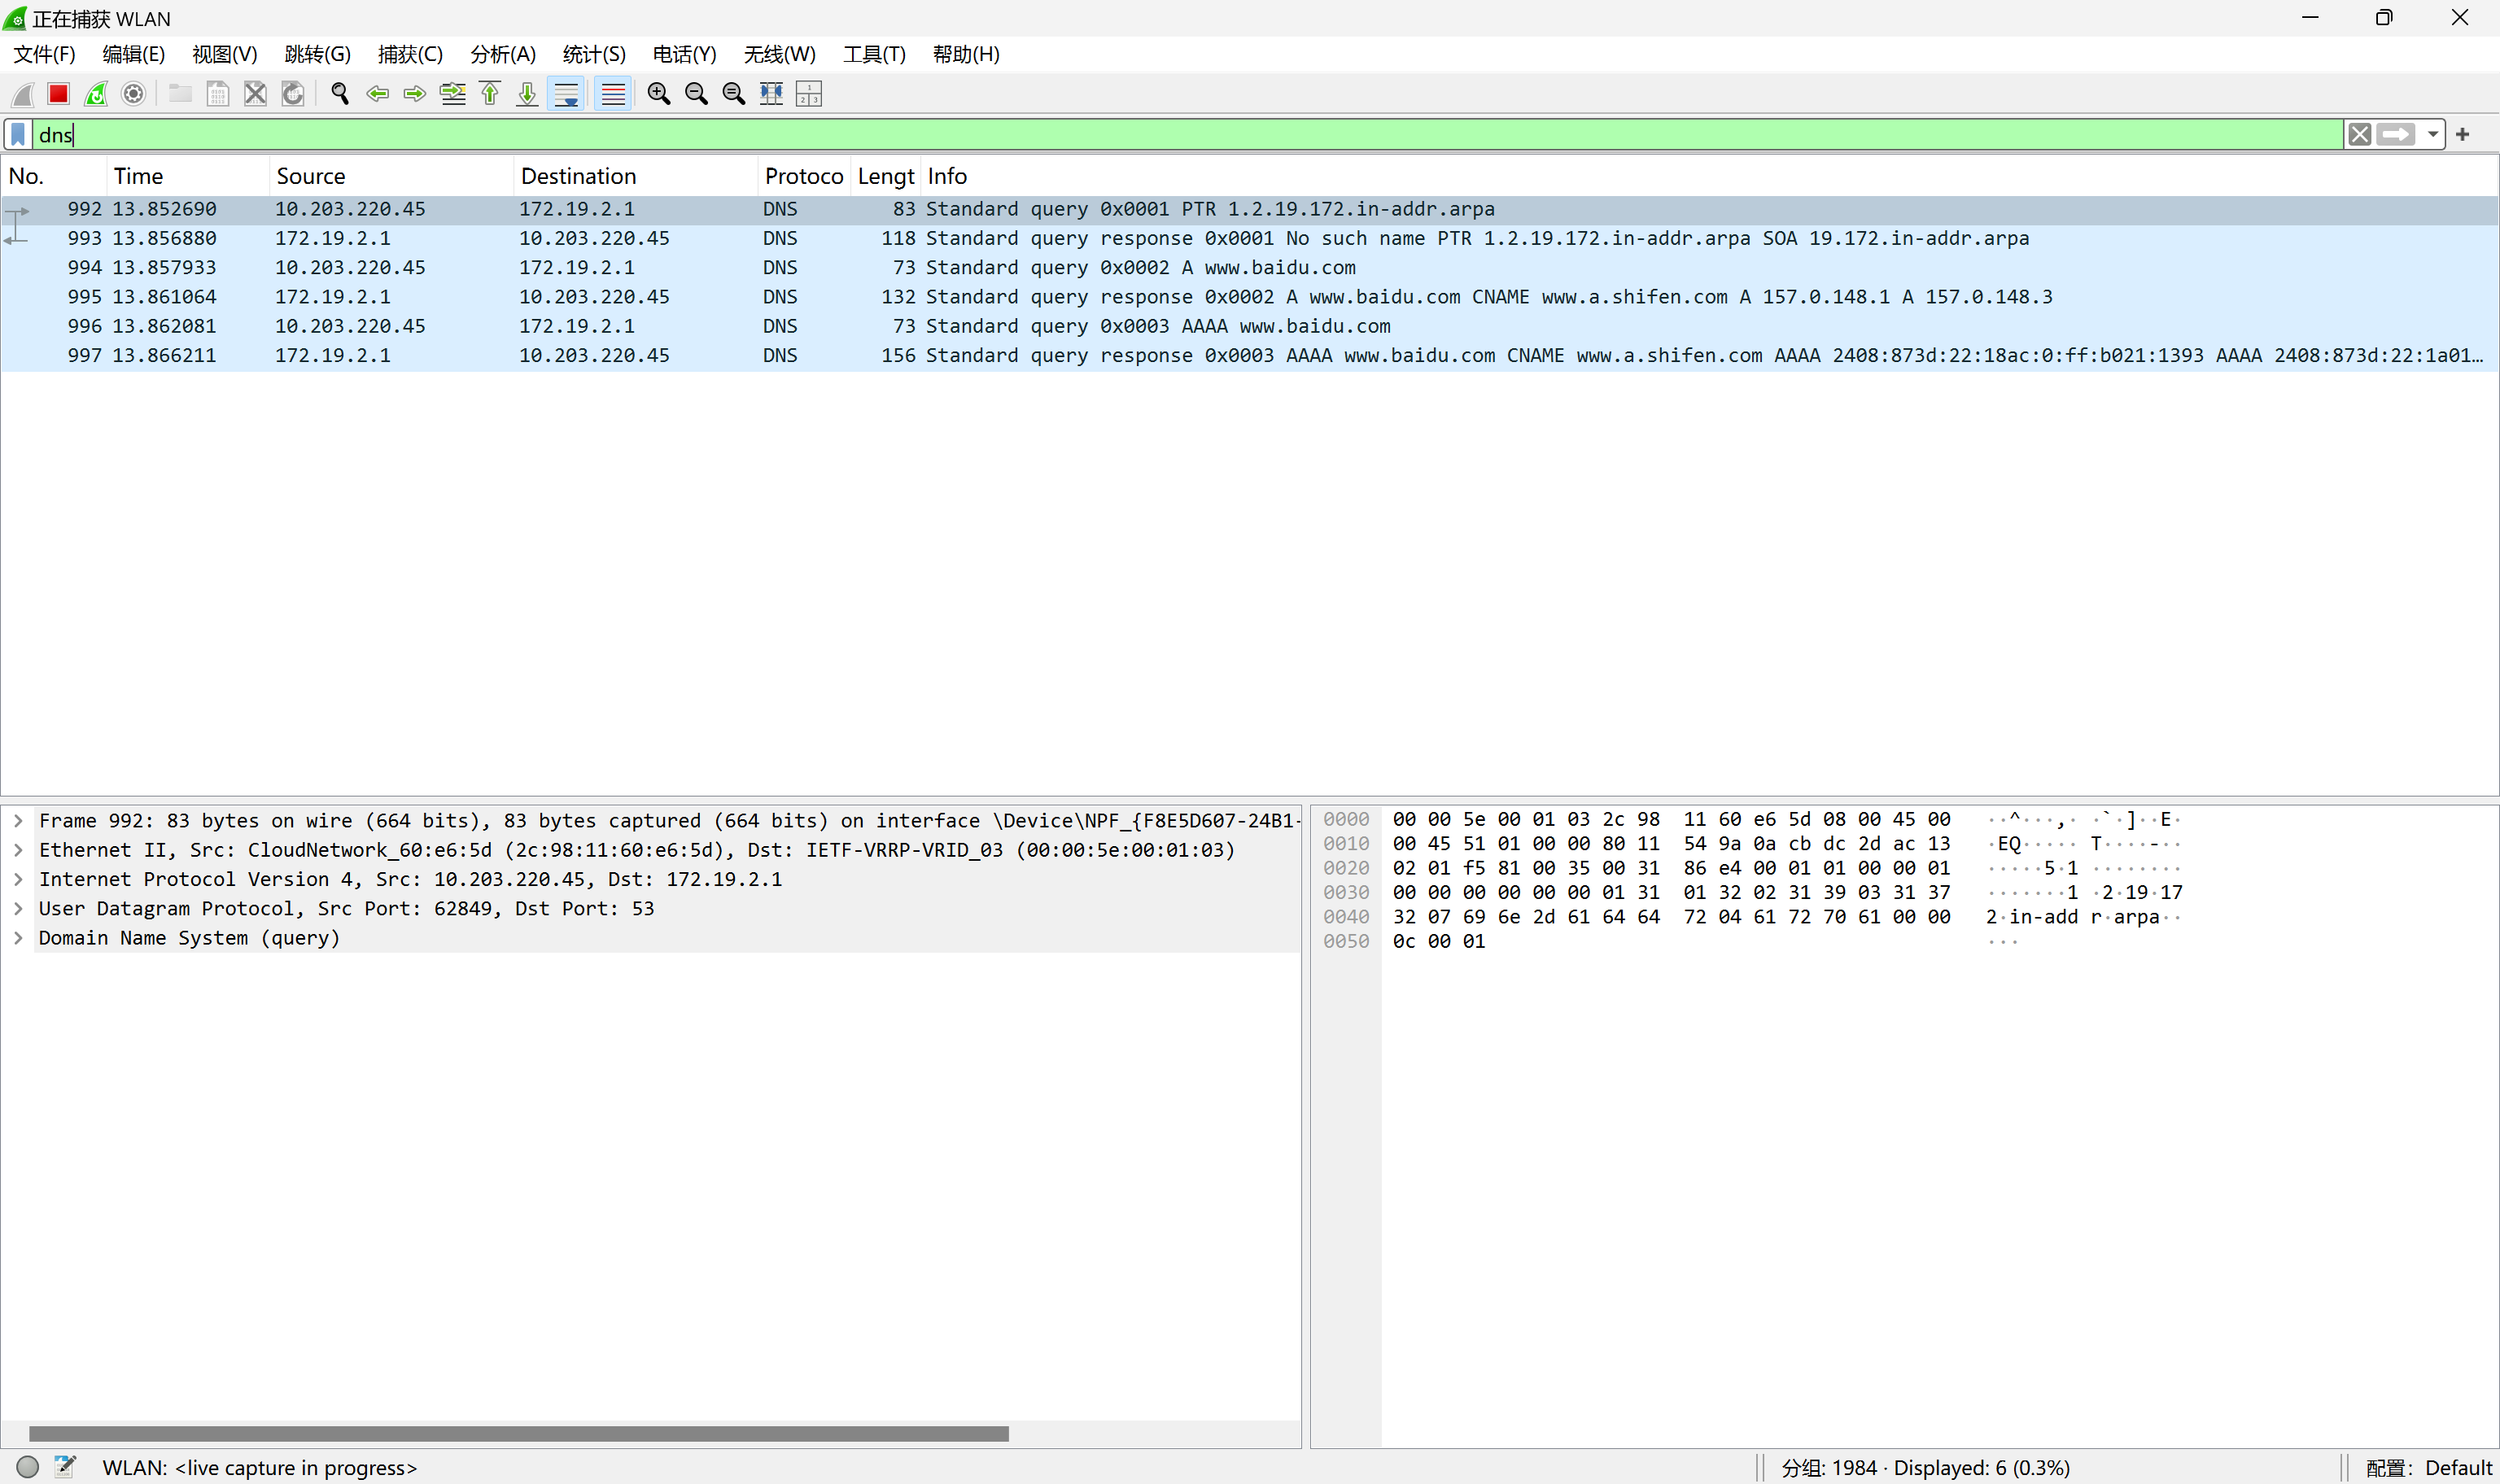
\includegraphics[width=0.8\textwidth]{1_1_images/21.png}}
\vspace{10pt}

\subsection{心得体会}
通过这次实验,我深入学习并实践了网络协议、数据包捕获、域名解析和网络路径追踪等关键技能。使用Wireshark抓包软件,我掌握了如何设置捕获过滤器和显示过滤器,这让我能够精确地分析HTTP和DNS协议的数据包。我还尝试了curl命令来访问网页,并通过telnet命令体验了HTTP和SMTP服务的交互过程。tracert命令让我了解了数据包在网络中的路径和可能的延迟点,而nslookup则帮助我查询和分析了域名信息。这些工具和技能不仅增强了我的网络分析能力,也让我对网络通信的复杂性和精妙性有了更深的认识。总的来说,这次实验是一次宝贵的学习经历,它不仅提升了我的技术能力,也激发了我对网络技术进一步探索的兴趣。

\newpage\section{实验1.2 TCP协议分析}
\subsection{实验目的}
TCP(Transmission Control Protocol 传输控制协议)是一种面向连接的、可靠的、基于字节流的传输层通信协议。本实验通过运用 Wireshark 对网络活动进行分析,观察TCP 协议报文,分析通信时序,理解 TCP 的工作过程,掌握 TCP 工作原理与实现;学会运用 Wireshark 分析 TCP 连接管理、流量控制和拥塞控制的过程,发现 TCP 的性能问题。
\subsection{实验内容}
观察 TCP 三次握手与四次挥手报文,注意报文收发过程中,双方 TCP 状态的变化。以本次捕获的报文为依据,分别画出本次 TCP 连接三次握手与四次挥手的时序图,结合 TCP 状态机,在双方各阶段标出对应的TCP 状态。选择其中一个TCP 报文,配合Wireshark 截图,分析该报文 TCP 首部各字段的定义、值及其含义。
\begin{itemize}
    \item TCP 数据流的追踪
    \item TCP 连接的建立
    \item TCP 连接的终止
    \item TCP 连接的重置
\end{itemize}
\subsection{小组成员及分工}
本次实验为单人实验
\subsection{实验过程与结果分析}
\subsubsection{TCP建立连接三次握手报文}
这里客户端为10.208.123.215,服务器端为20.189.173.8。
1.客户端向服务器端发送SYN包。
客户端发送一个SYN包(SYN标志位为1,序列号Seq=0)给服务器端,客户端的TCP状态从CLOSED变为SYN-SENT。
2.服务器端回应客户端的SYN包并且发送自己的SYN包。
服务器端收到客户端的SYN包后,发送一个SYN+ACK包给客户端,其中SYN和ACK标志位都为1,确认号Ack=0+1=1,序列号Seq=1。服务器端的TCP状态从CLOSED变为SYN-RECEIVED。
3.客户端发送确认包给服务器端。
客户端收到服务器端的SYN+ACK包后,发送一个ACK包给服务器端,其中ACK标志位为1,确认号Ack=1,序列号Seq=1。客户端的TCP状态从SYN-SENT变为ESTABLISHED,并且当服务器端收到客户端的ACK包后,TCP状态从SYN-RECEIVED变为ESTABLISHED。

\vspace{10pt}
\centerline{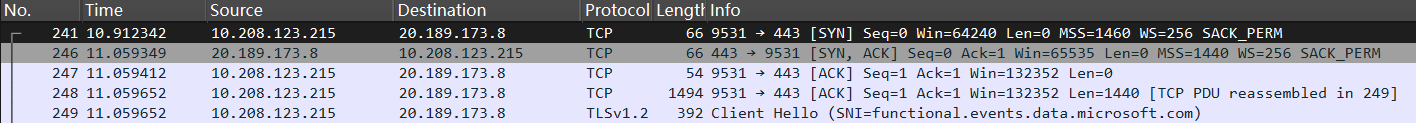
\includegraphics[width=0.8\textwidth]{1_2_images/1.png}}
\vspace{10pt}

\subsubsection{TCP断开连接四次挥手报文}
这里客户端为:2408:873c:4810:4:8000:0:b00:31,
服务器端为:240c:c603:d:d480:e9fd:a970:17b:8017。
1.客户端发送FIN包
客户端向服务器端发送一个FIN包(FIN标志位为1,序列号Seq=25,Ack=1)开始关闭连接。客户端的TCP状态从ESTABLISHED变为FIN-WAIT-1。
2.服务器端确认客户端的FIN包
服务器端收到客户端的FIN包后,发送一个ACK包(序列号Seq=1,ACK标志位为1,确认号Ack=25+1=26)给客户端,表示收到了关闭请求。服务器端的TCP状态从ESTABLISHED变为CLOSE-WAIT。
3.服务器端发送自己的FIN包
服务器端在准备关闭连接时,向客户端发送一个FIN包(FIN标志位为1,序列号Seq=1,Ack=25+1=26)。服务器端的TCP状态从CLOSE-WAIT变为LAST-ACK。
④客户端确认服务器端的FIN包
客户端收到服务器端的FIN包后,发送一个ACK包(序列号Seq=25+1=26,ACK标志位为1,确认号Ack=1+1=2)给服务器端。客户端的TCP状态从FIN-WAIT-1变为TIME-WAIT,等待2MSL(Maximum Segment Lifetime)后关闭连接。服务器端收到客户端的ACK包后,TCP连接关闭,服务器端的TCP状态从LAST-ACK变为CLOSED。

\vspace{10pt}
\centerline{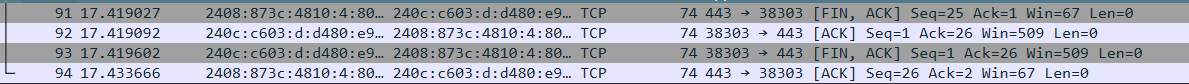
\includegraphics[width=0.8\textwidth]{1_2_images/2.png}}
\vspace{10pt}

\subsubsection{分析建立TCP连接时,客户端向服务器端发送的第一条报文}
在Transmission Control Protocol中,源端口号为9531,目的端口号为443,Seq=0,代表初次连接,并且Acknowledgment Number=0,说明Ack=0。此外,在Flags中,SYN=1,表示请求建立连接。

\vspace{10pt}
\centerline{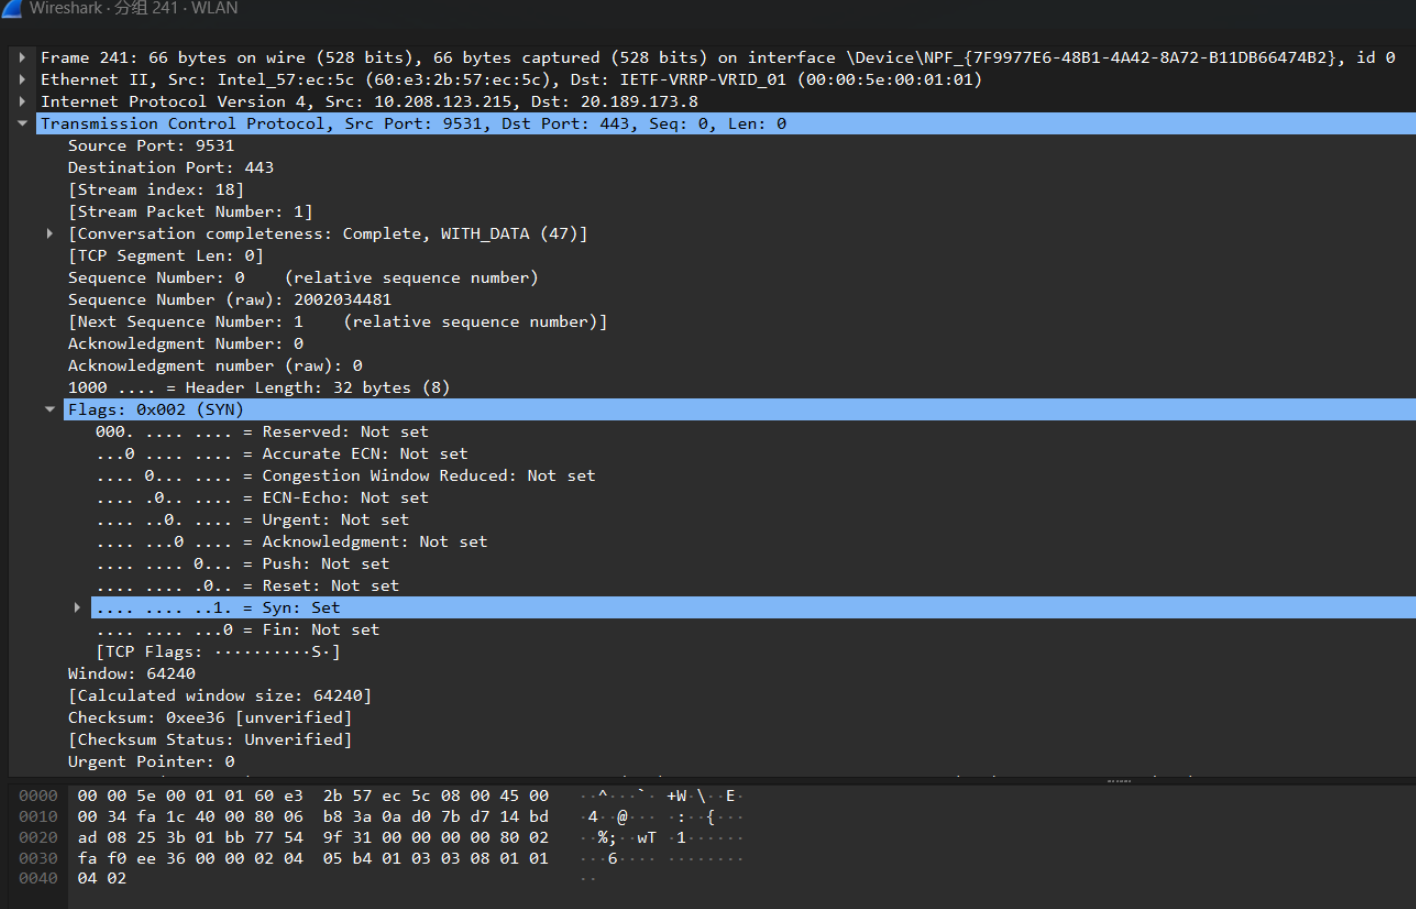
\includegraphics[width=0.8\textwidth]{1_2_images/3.png}}
\vspace{10pt}

\subsubsection{三次握手与四次挥手的时序图以及TCP状态}

\vspace{10pt}
\centerline{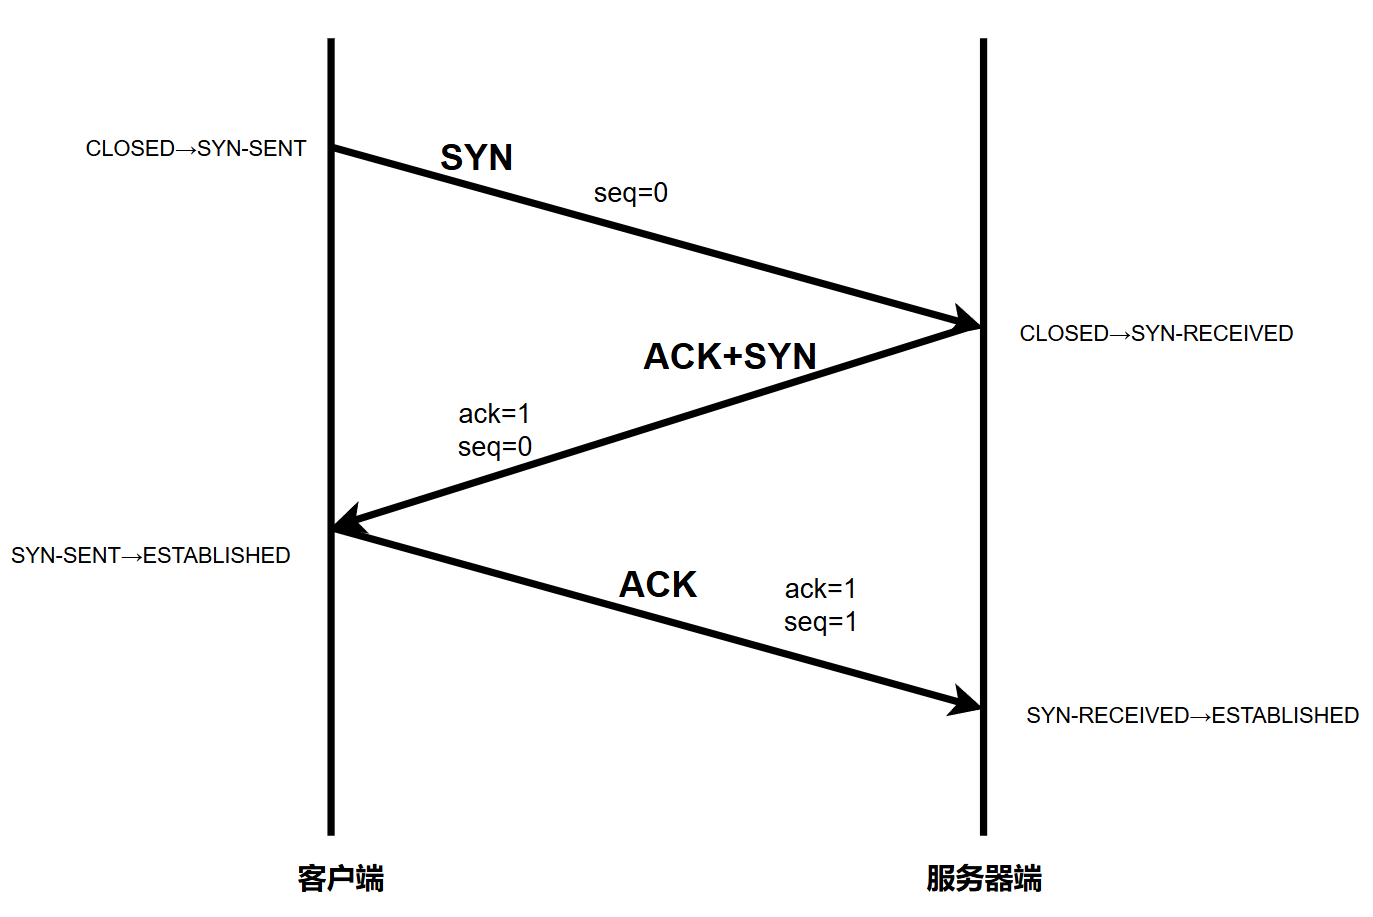
\includegraphics[width=0.8\textwidth]{1_2_images/4.png}}
\vspace{10pt}

\vspace{10pt}
\centerline{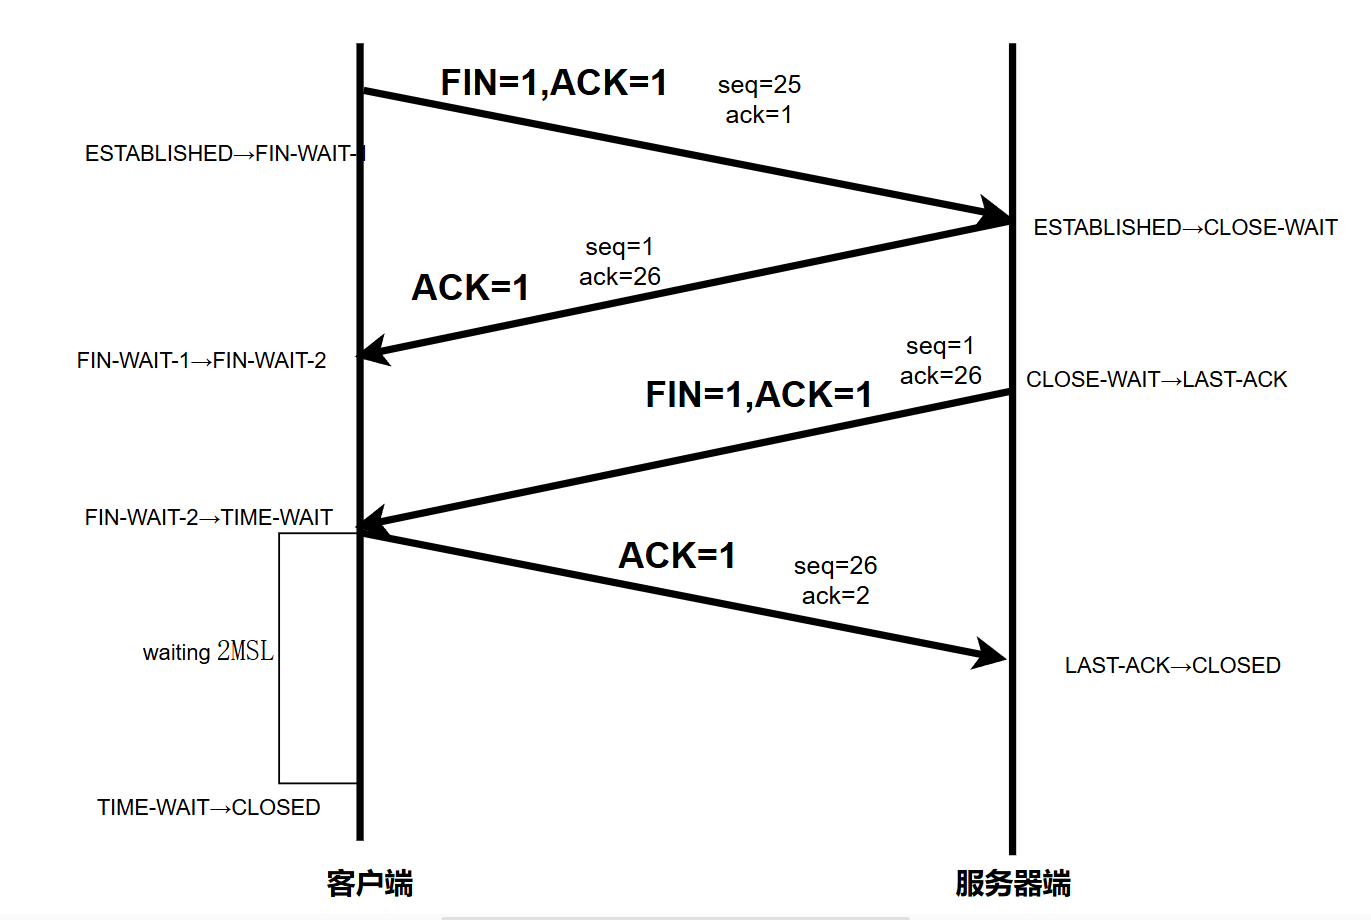
\includegraphics[width=0.8\textwidth]{1_2_images/5.png}}
\vspace{10pt}

\subsubsection{TCP连接的重置}
使用Wireshark 过滤显示RST置位数据包,即使用:tcp.flags.reset == 1。筛选结果如图38所示。点开第4条报文,查看其详细信息。在Flags栏中,Reset为set状态,说明这是一条异常中止的报文,可以使TCP快速断开。

\vspace{10pt}
\centerline{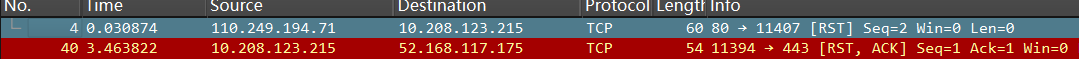
\includegraphics[width=0.8\textwidth]{1_2_images/6.png}}
\vspace{10pt}

\vspace{10pt}
\centerline{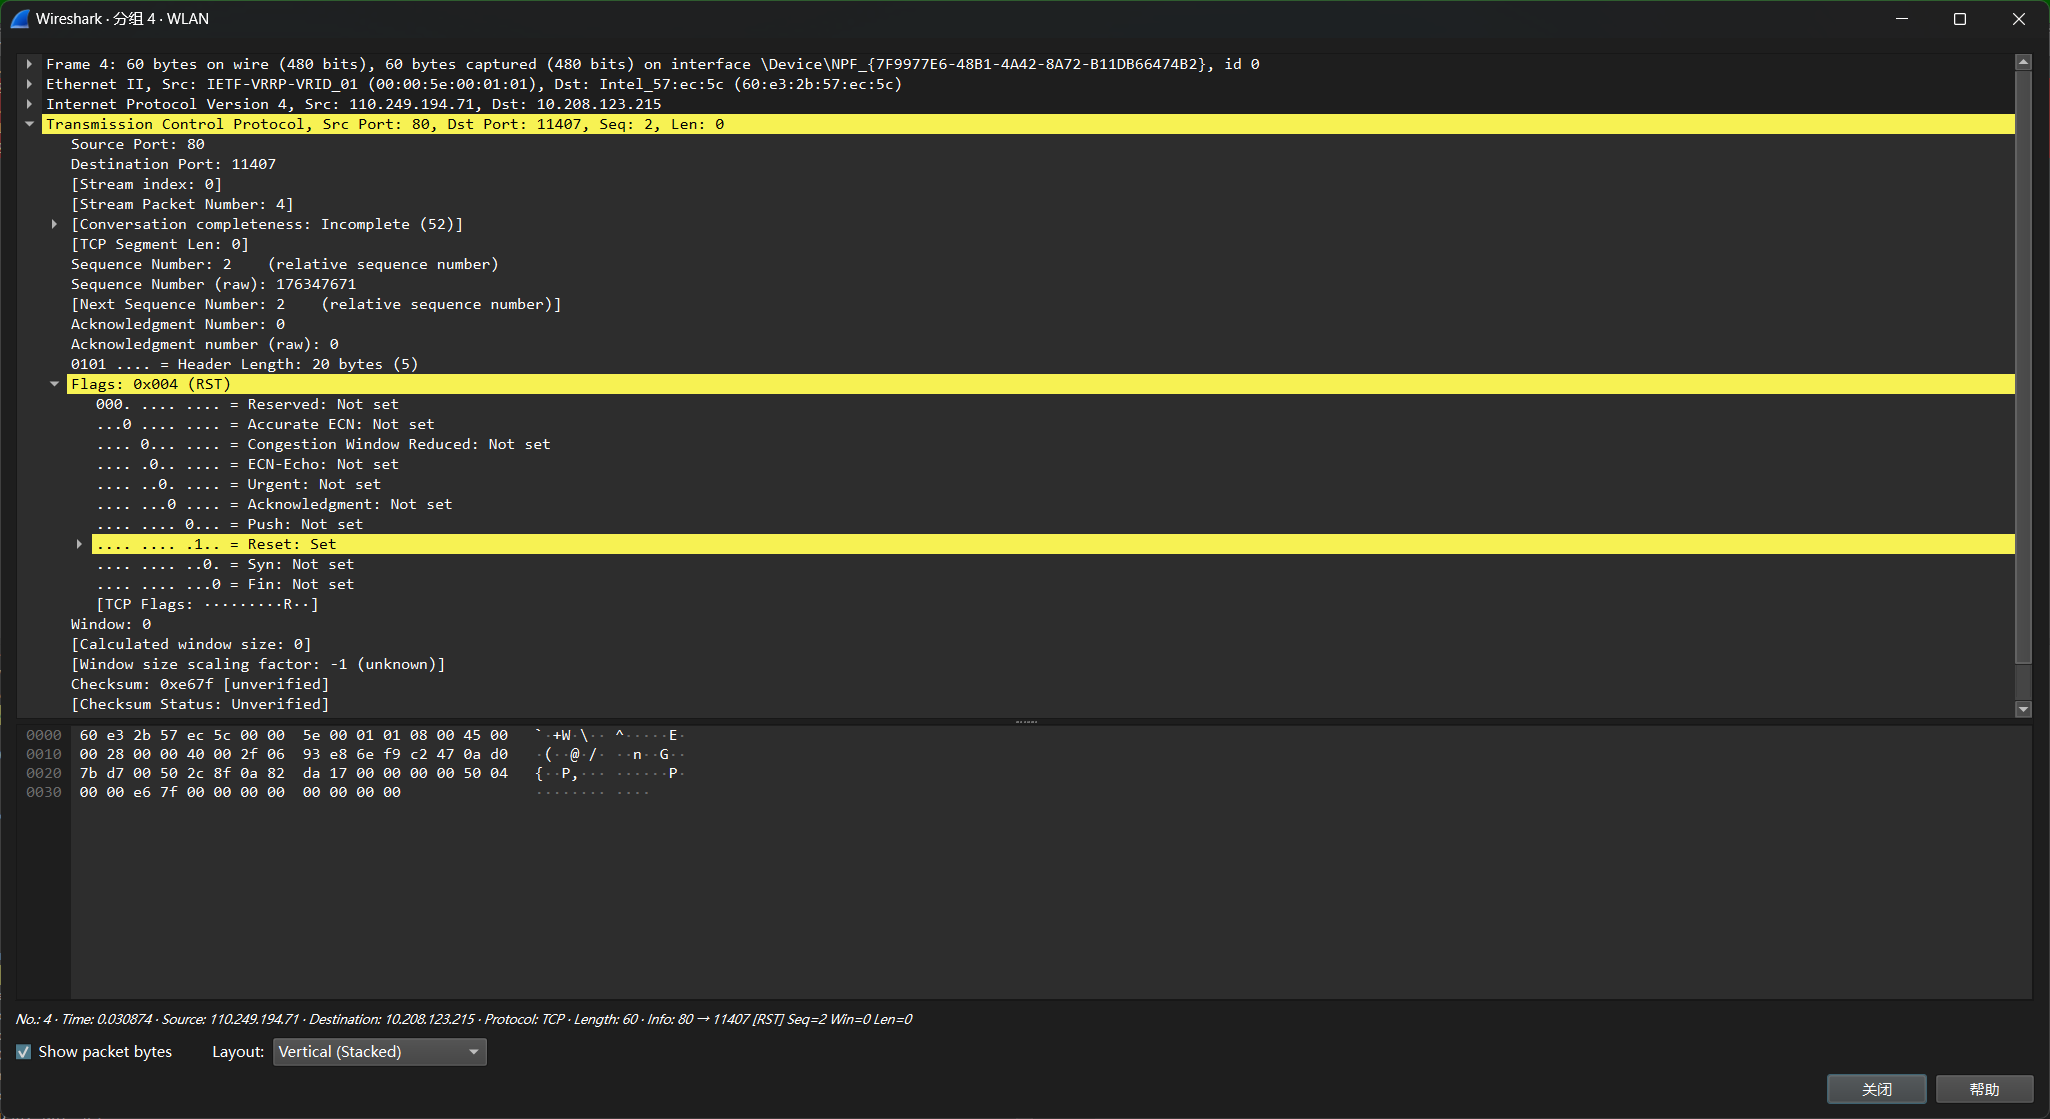
\includegraphics[width=0.8\textwidth]{1_2_images/7.png}}
\vspace{10pt}

\subsection{心得体会}
1、更加深入理解TCP连接的建立与断开过程。通过实际抓包分析和时序图的绘制,加深了对TCP连接建立和断开过程的理解。了解三次握手和四次挥手的具体步骤,以及每个步骤中TCP状态的变化。并且了解到了TCP异常中止以及TCP连接重置的相关知识。
2、认识到了TCP状态机对网络协议的设计及其运行机制至关重要,能帮助解决实际网络问题。
3、更加熟练使用Wireshark,认识到使用Wireshark等工具捕获和分析TCP报文有助于深入理解网络通信过程,尤其是在故障排查时。




\newpage\section{实验2.1 物理连通实验(制作网线)}
\subsection{实验目的}
掌握 Gbit/s 速率直通网线的制作方法,熟练使用相关工具完成网线制作各步骤,保证网线质量符合要求且线序正确、连接可靠。
\subsection{实验内容}
\begin{itemize}
    \item 方案:
    \item 制作一根传输速率为 Gbit/s 的以太网线,作为后续实验链路。
    \item 网线分为直通网线(Straight through cable)和交叉网线
    (Crossover cable)两种,当前绝大部分网卡/设备都支持自适应线序,本实验只需要制作直通网线。
    \item 验收:
    \item 使用网线测试仪,监测网线状态。
    \item 网线接入网卡中,查看网卡状态是否正常。
\end{itemize}
\subsection{小组成员及分工}
本次实验为单人实验,无分工。
\subsection{实验过程与结果分析}
1.使用网线钳剪下约一米长的网线,并使用剥线钳拨开约 1.5 厘米长的外皮。

2.按照 T568B 线序理线,颜色依次是橙白、橙色、绿白、蓝色、蓝白、绿色、棕白、棕色。

3.使用网线钳减去头部线缆,使其对齐。

4.将线缆插入水晶头并确保线缆插到底部。

5.将水晶头伸入网线钳用力压紧。

6.同样的方法制作网线另一端。

7.用测线仪对做好的网线进行检测,确认信号灯能够正确闪亮。
\subsection{实验思考:物理层确定的接口特性}
实验所用线材应该是双绞线与非屏蔽线,接线器是水晶头RJ45连接器。
\subsection{心得体会}
这次实验内容并不复杂,但是耗费了我们很长时间和很多精力,总结经验在于细节把握不仔细,导致线的连接有问题,主要应该关注怎么精准地剥皮和对齐线缆,怎么在压接水晶头时确保每根线缆都紧密接触,避免出现接触不良的情况。实验不仅提高了我的动手能力,还让我对网络设备的配置和故障排查有了更多的认识,对我未来的学习很有帮助。


\newpage\section{实验2.2 2台PC直连组网}
\subsection{实验目的}
通过在两台PC之间进行直连组网,理解并应用网络通信协议和以太网技术。
\subsection{实验内容}
\begin{itemize}
    \item 确定PC机可支持的网卡类型,选择物理通道。网卡可以有多种选择,本实验均采用以太网卡+网线方式。
    \item 确定使用的通信协议。本实验PC间可使用非IP协议通信,后续实验都采用事实标准IP协议。
    \item PC使用xcap模拟发送以太报文(设置为非IP包,例如用IPX协议):
        \begin{itemize}
            \item 目的MAC设置为广播MAC。
            \item 目的MAC设置为对端PC机MAC。
            \item 目的MAC设置为未知的单播MAC。
        \end{itemize}
\end{itemize}
\subsection{小组成员及分工}
小组共三名成员,互相进行收发包的操作,共同完成实验。在实验报告中举出其中一组实验,分别将两台电脑命名为A和B,其中配置静态IP地址,A的IP地址为192.168.0.4,B的IP地址为192.168.0.3:

A电脑(梁耀欣):IP为192.168.0.4

B电脑(李昶瑾):IP为192.168.0.3
\subsection{实验过程与结果分析}
使用网线连接两台电脑的网口:
\subsubsection{两台电脑ping并抓包}
A电脑向B电脑发出ping请求:
\begin{center}
    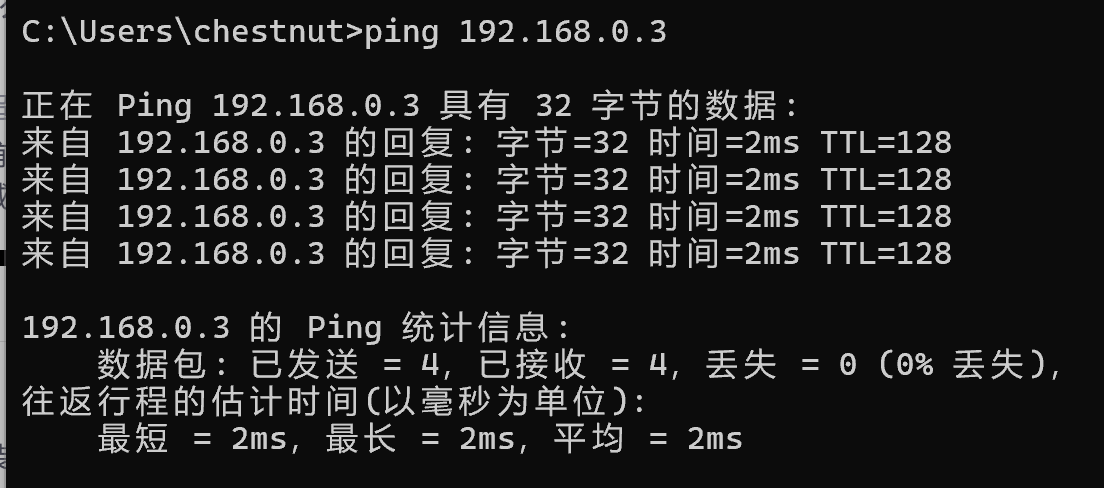
\includegraphics[width=0.8\textwidth]{2_2_images/2.png}
\end{center}

B电脑向A电脑发出ping请求:
\begin{center}
    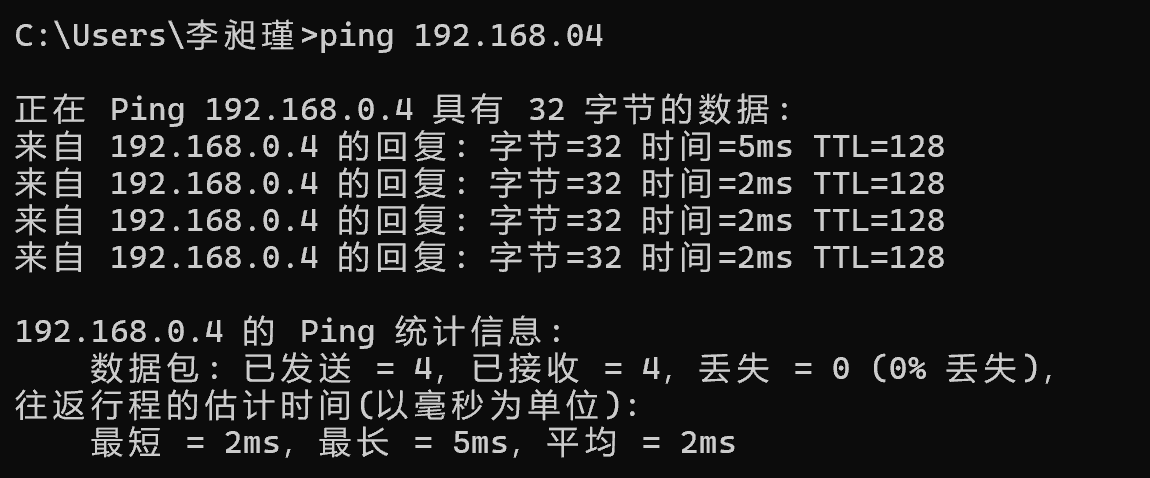
\includegraphics[width=0.8\textwidth]{2_2_images/1.png}
\end{center}

A电脑抓包结果:
\begin{center}
    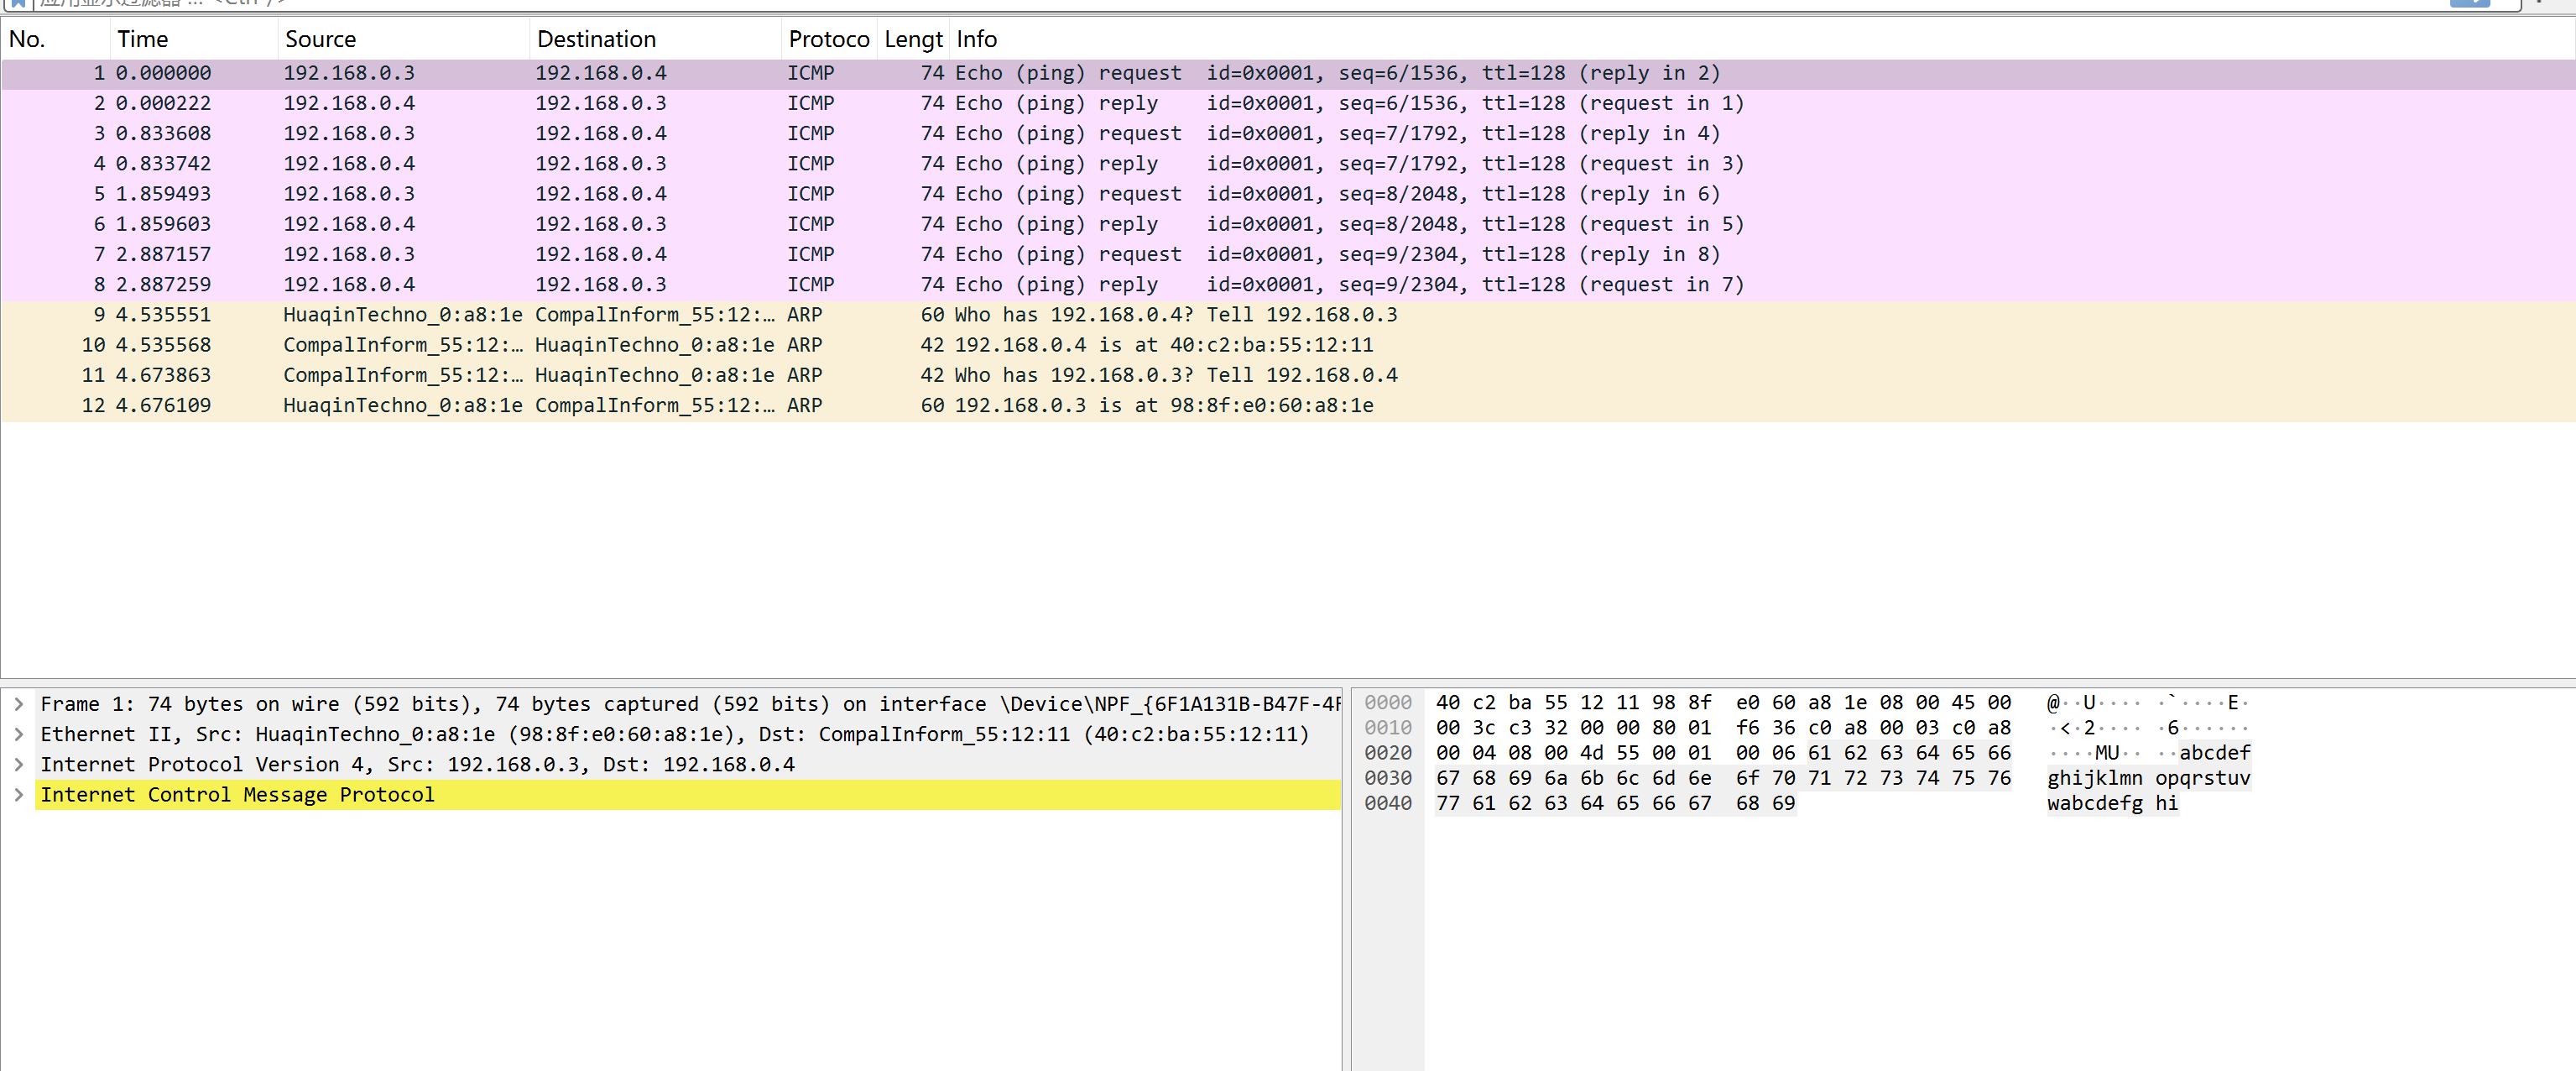
\includegraphics[width=1\textwidth]{2_2_images/3.png}
\end{center}

可以看出A电脑收到了四个B向A的请求的ICMP包,对每个包都有reply回应。

\subsubsection{使用小兵软件进行发包}
\begin{itemize}
    \item 打开小兵软件,在主页面的左侧的配置处双击新建流。
    \item 在报文编辑页面选择以太网,编辑内容中的源MAC地址和目的MAC地址。
    \item 点击确定保存配置,然后勾选这个配置点击发送报文,就可以发包。
    \item MAC地址可以在命令行中用“ipconfig”命令读取到
    
    \begin{center}
        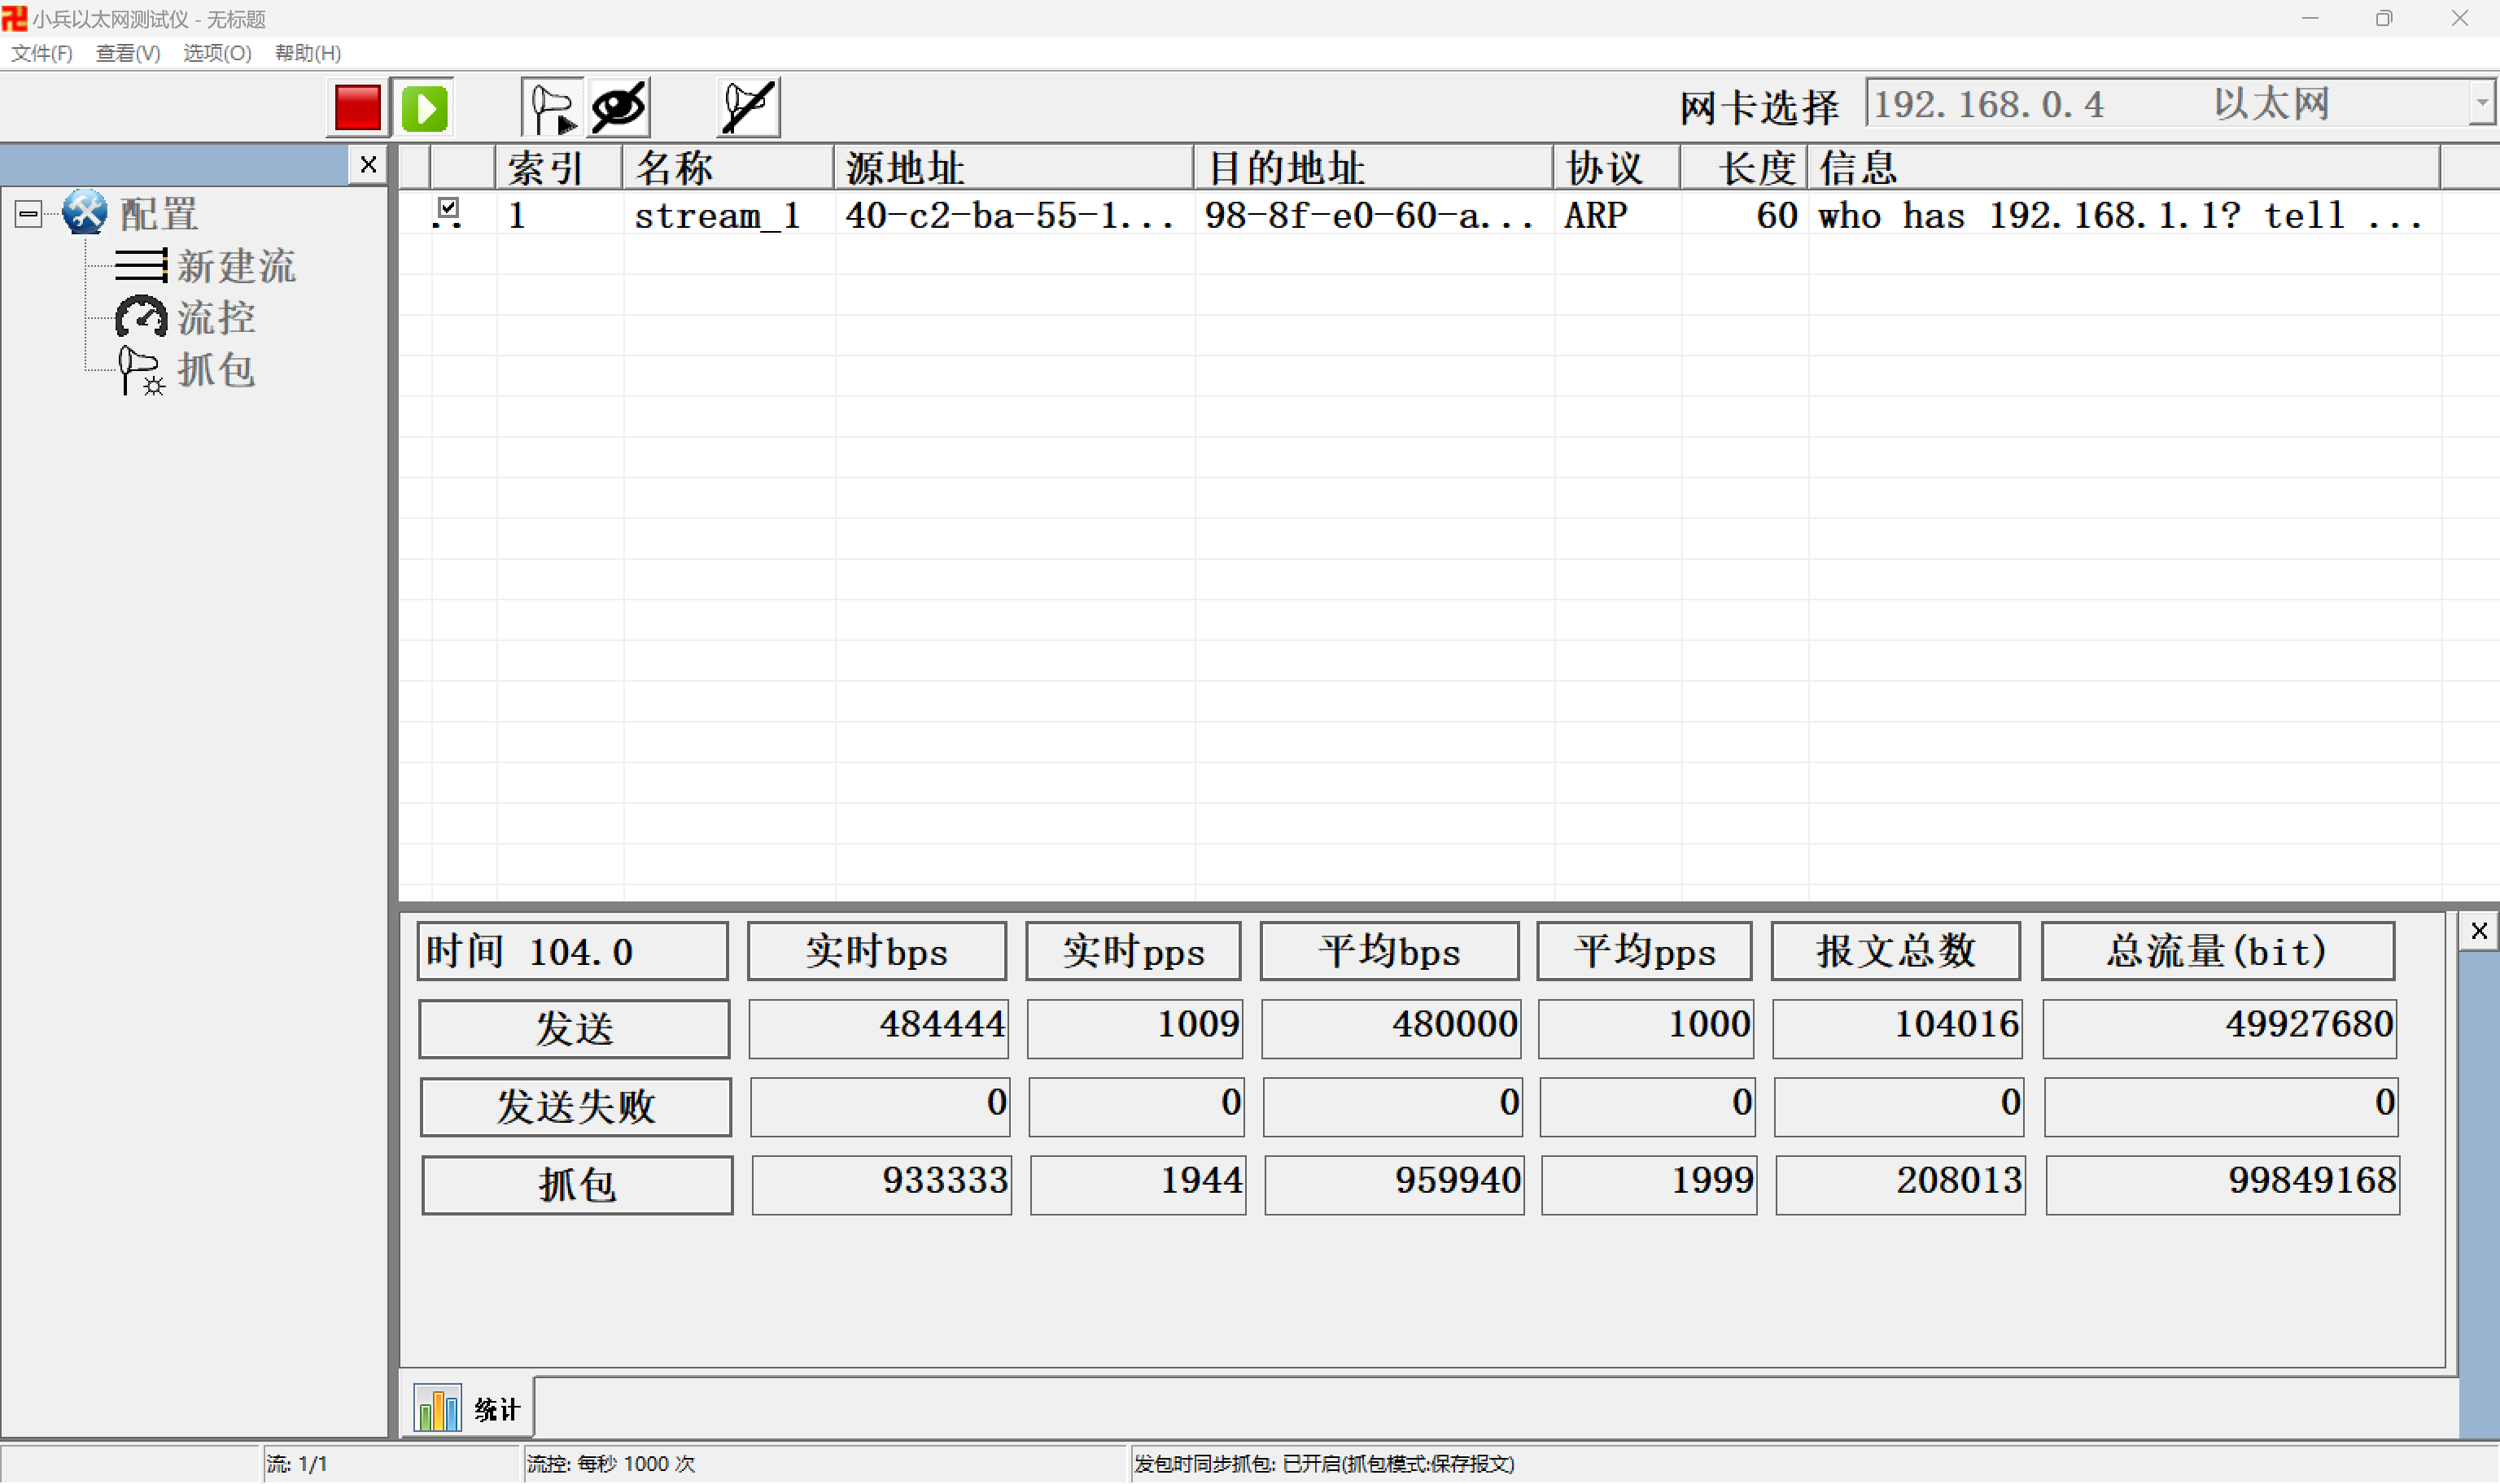
\includegraphics[width=0.8\textwidth]{2_2_images/4.png}
    \end{center}
    
    \begin{itemize}
        \item 目的MAC设置为对端PC机MAC:在A上启动发包,在B上启动收包,此时A和B会收到来自A的以太包。
        
        \begin{center}
            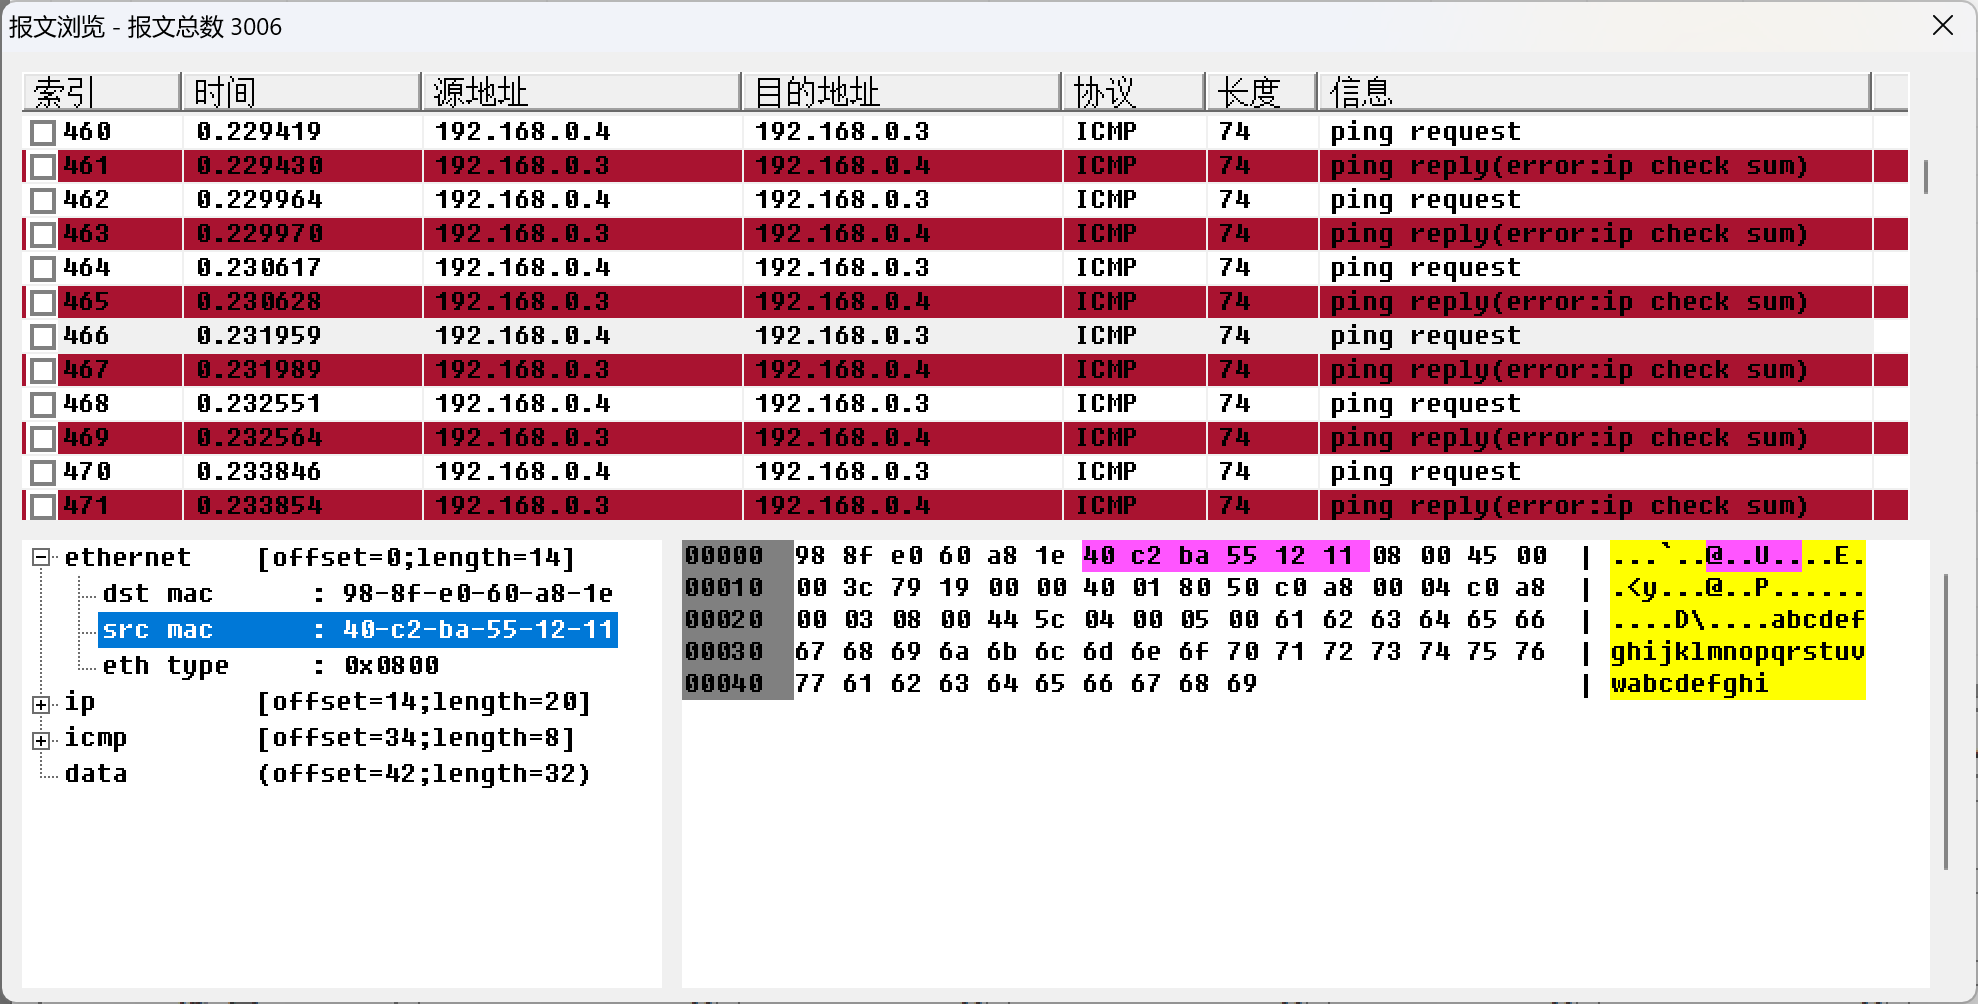
\includegraphics[width=0.8\textwidth]{2_2_images/8.png}
        \end{center}
        
        \item 目的MAC设置为广播MAC:把目的MAC地址设置为FF:FF:FF:FF:FF:FF。在B上启动发包,在A上启动收包,此时A和B会收到来自B的广播包。设备不知道目标 IP 地址对应的MAC地址时,发送 ARP 请求到广播地址,以便网络上的所有设备都能接收到这个请求。
        
        \begin{center}
            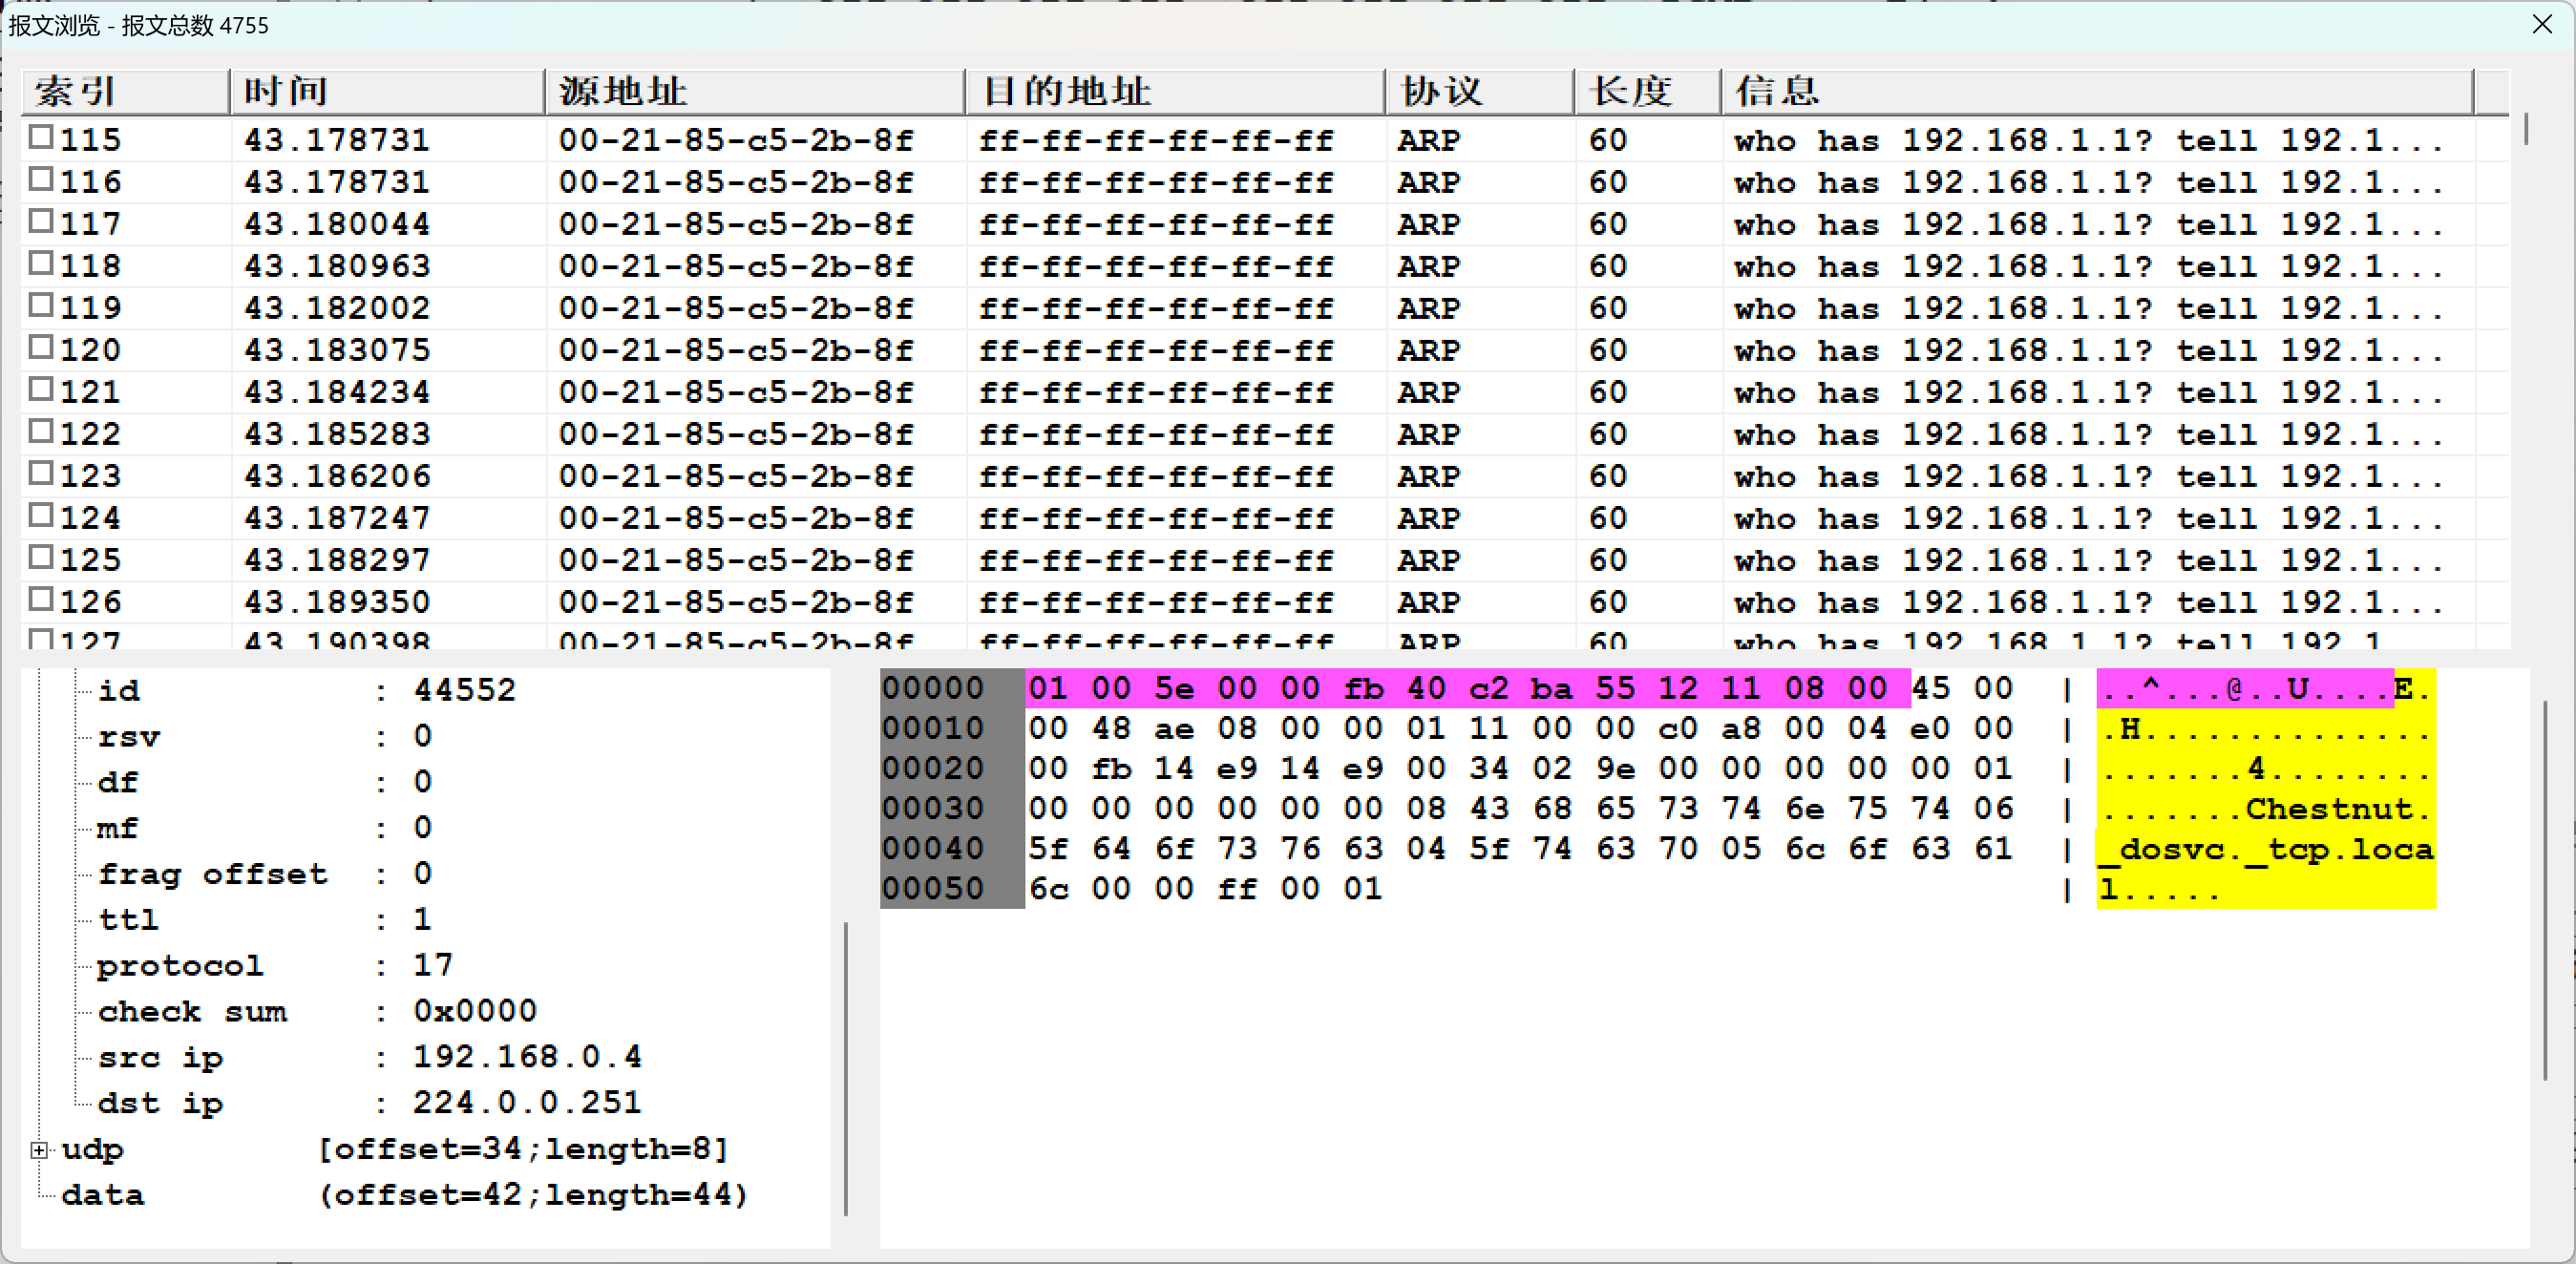
\includegraphics[width=0.8\textwidth]{2_2_images/6.png}
        \end{center}
        
        \item 目的MAC设置为未知单播MAC:在B上启动发包,在A上启动收包,此时虽然MAC地址是单播报文,但是由于ARP表为空,需要找到对应的IP地址,所以会收到ARP请求。但是由于报文是单播,其他PC无法收到ARP回复。
        
        \begin{center}
            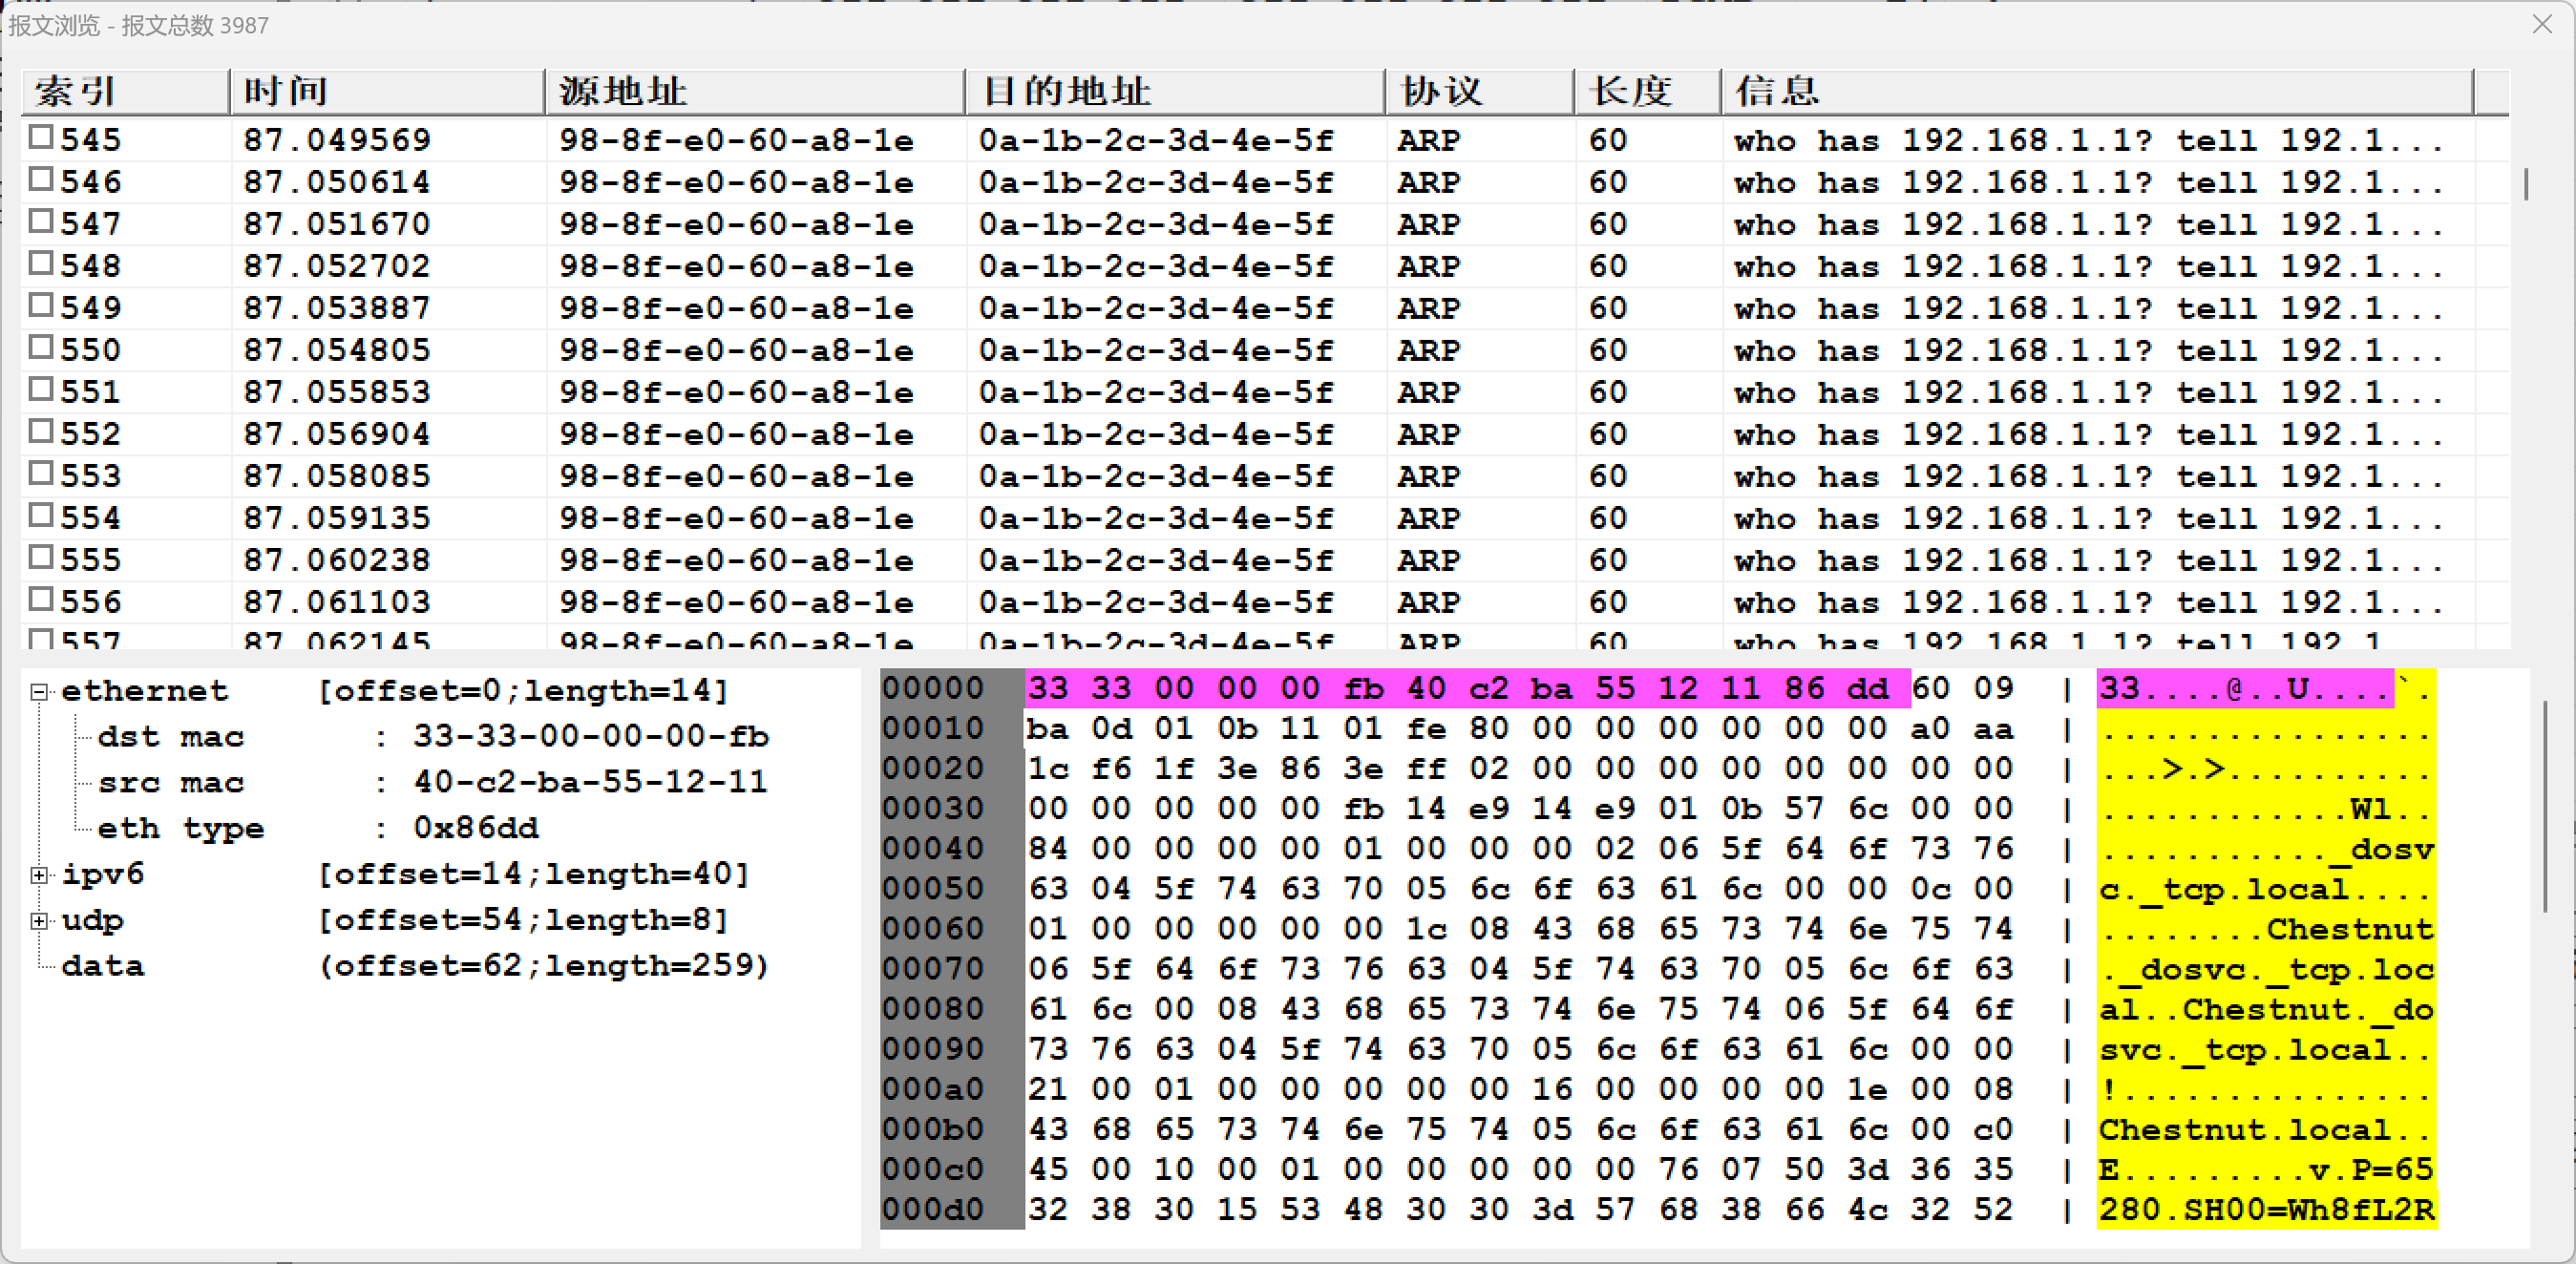
\includegraphics[width=0.8\textwidth]{2_2_images/7.png}
        \end{center}
    \end{itemize}
\end{itemize}
\subsubsection{实验错误的纠正过程}
在设置报文的时候,我们犯了一个错误,就是把 ARP 的
目的 IP 地址写成了 192.168.1.1,导致 IP 地址(同样也是对应MAC地址)的主机抓包只能抓到ARP 请求,抓不到 ARP 回复。经过调整之后,我们可以成功抓到ARP报文的回复。
实验成功。
\subsection{实验思考}
\begin{itemize}
    \item \textbf{Q: 抓包看到的以太网帧,与物理链路上传输的数据,有哪些差异?}
    \item \textbf{A:} 信号形式的差异,在物理链路上是以光信号或电信号的形式在物理介质中传输的模拟信号或数字信号,而抓包工具看到的以太网帧是这些信号被网卡接收并转换为数字数据后的形式;数据完整性的差异,物理链路上可能由于一些丢包和损坏衰减等导致错误的数据包,抓包工具看到的以太网帧通常只显示成功接收并经过校验的数据包。
\end{itemize}

\subsection{心得体会}
在实验中,我们通过小兵软件发送以太包,观察了以太包的发送和接收过程。通过观察,我们发现,当目的MAC地址为广播地址时,发送的以太包会通过网卡发送到所有的网络设备,包括本机。当目的MAC地址为未知的单播地址时,发送的以太包会通过网卡发送到所有的网络设备,包括本机,但是由于ARP表为空,需要找到对应的IP地址,所以会收到ARP请求。当目的MAC地址为对端PC的MAC地址时,发送的以太包会通过网卡发送到对端PC,但是由于对端PC没有收到这个以太包,所以不会进行任何处理。


\newpage\section{实验2.3 多PC通过集线器HUB组网}
\subsection{实验目的}
测试集线器HUB的功能,理解集线器HUB的工作原理。
\subsection{实验内容}
\begin{itemize}
    \item 交换机关闭MAC学习,广播转发,用来模拟HUB*(实验老师已经预置)。
    \item PC机间使用网线连接集线器HUB,实现互连。
    \item PC间使用xcap模拟发送以太报文(可以设置为非IP包)。
    
    \vspace{10pt}
    \centerline{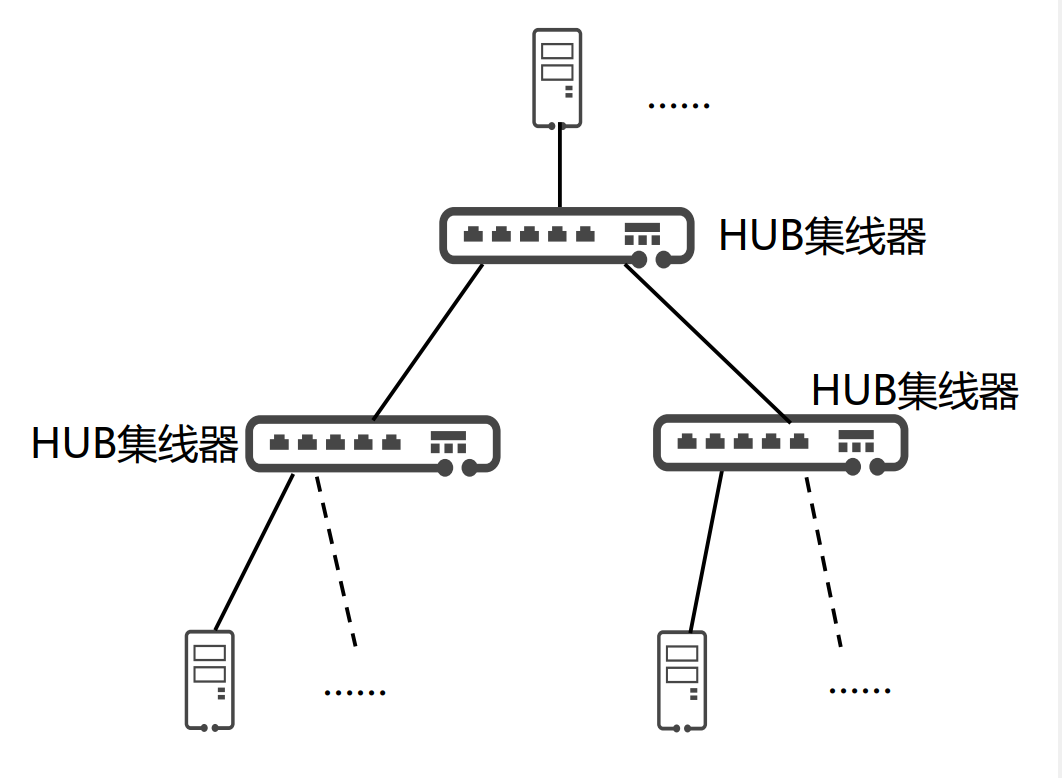
\includegraphics[width=0.5\textwidth]{2_2_images/9.png}}
    \vspace{10pt}
\end{itemize}

\subsection{小组成员及分工}
小组共三名成员,三台PC均连到HUB上,共同完成实验。

成员的PC机代号和IP配置如下:

梁耀欣: A: 192.168.0.4

李昶瑾: B: 192.168.0.3

赵露苗: C: 192.168.0.5

\subsection{实验过程与结果分析}
按照上面的拓扑图搭建好PC和交换机。
\subsubsection{设置交换机关闭MAC学习}
从用户模式切换到特权模式,进入VLAN1的配置模型,进入系统视图,使用命令
\begin{lstlisting}
system -view
vlan 1
mac-address learning disable
\end{lstlisting}
选择要配置的网络接口然后禁用交换机自学习功能:
\begin{center}
    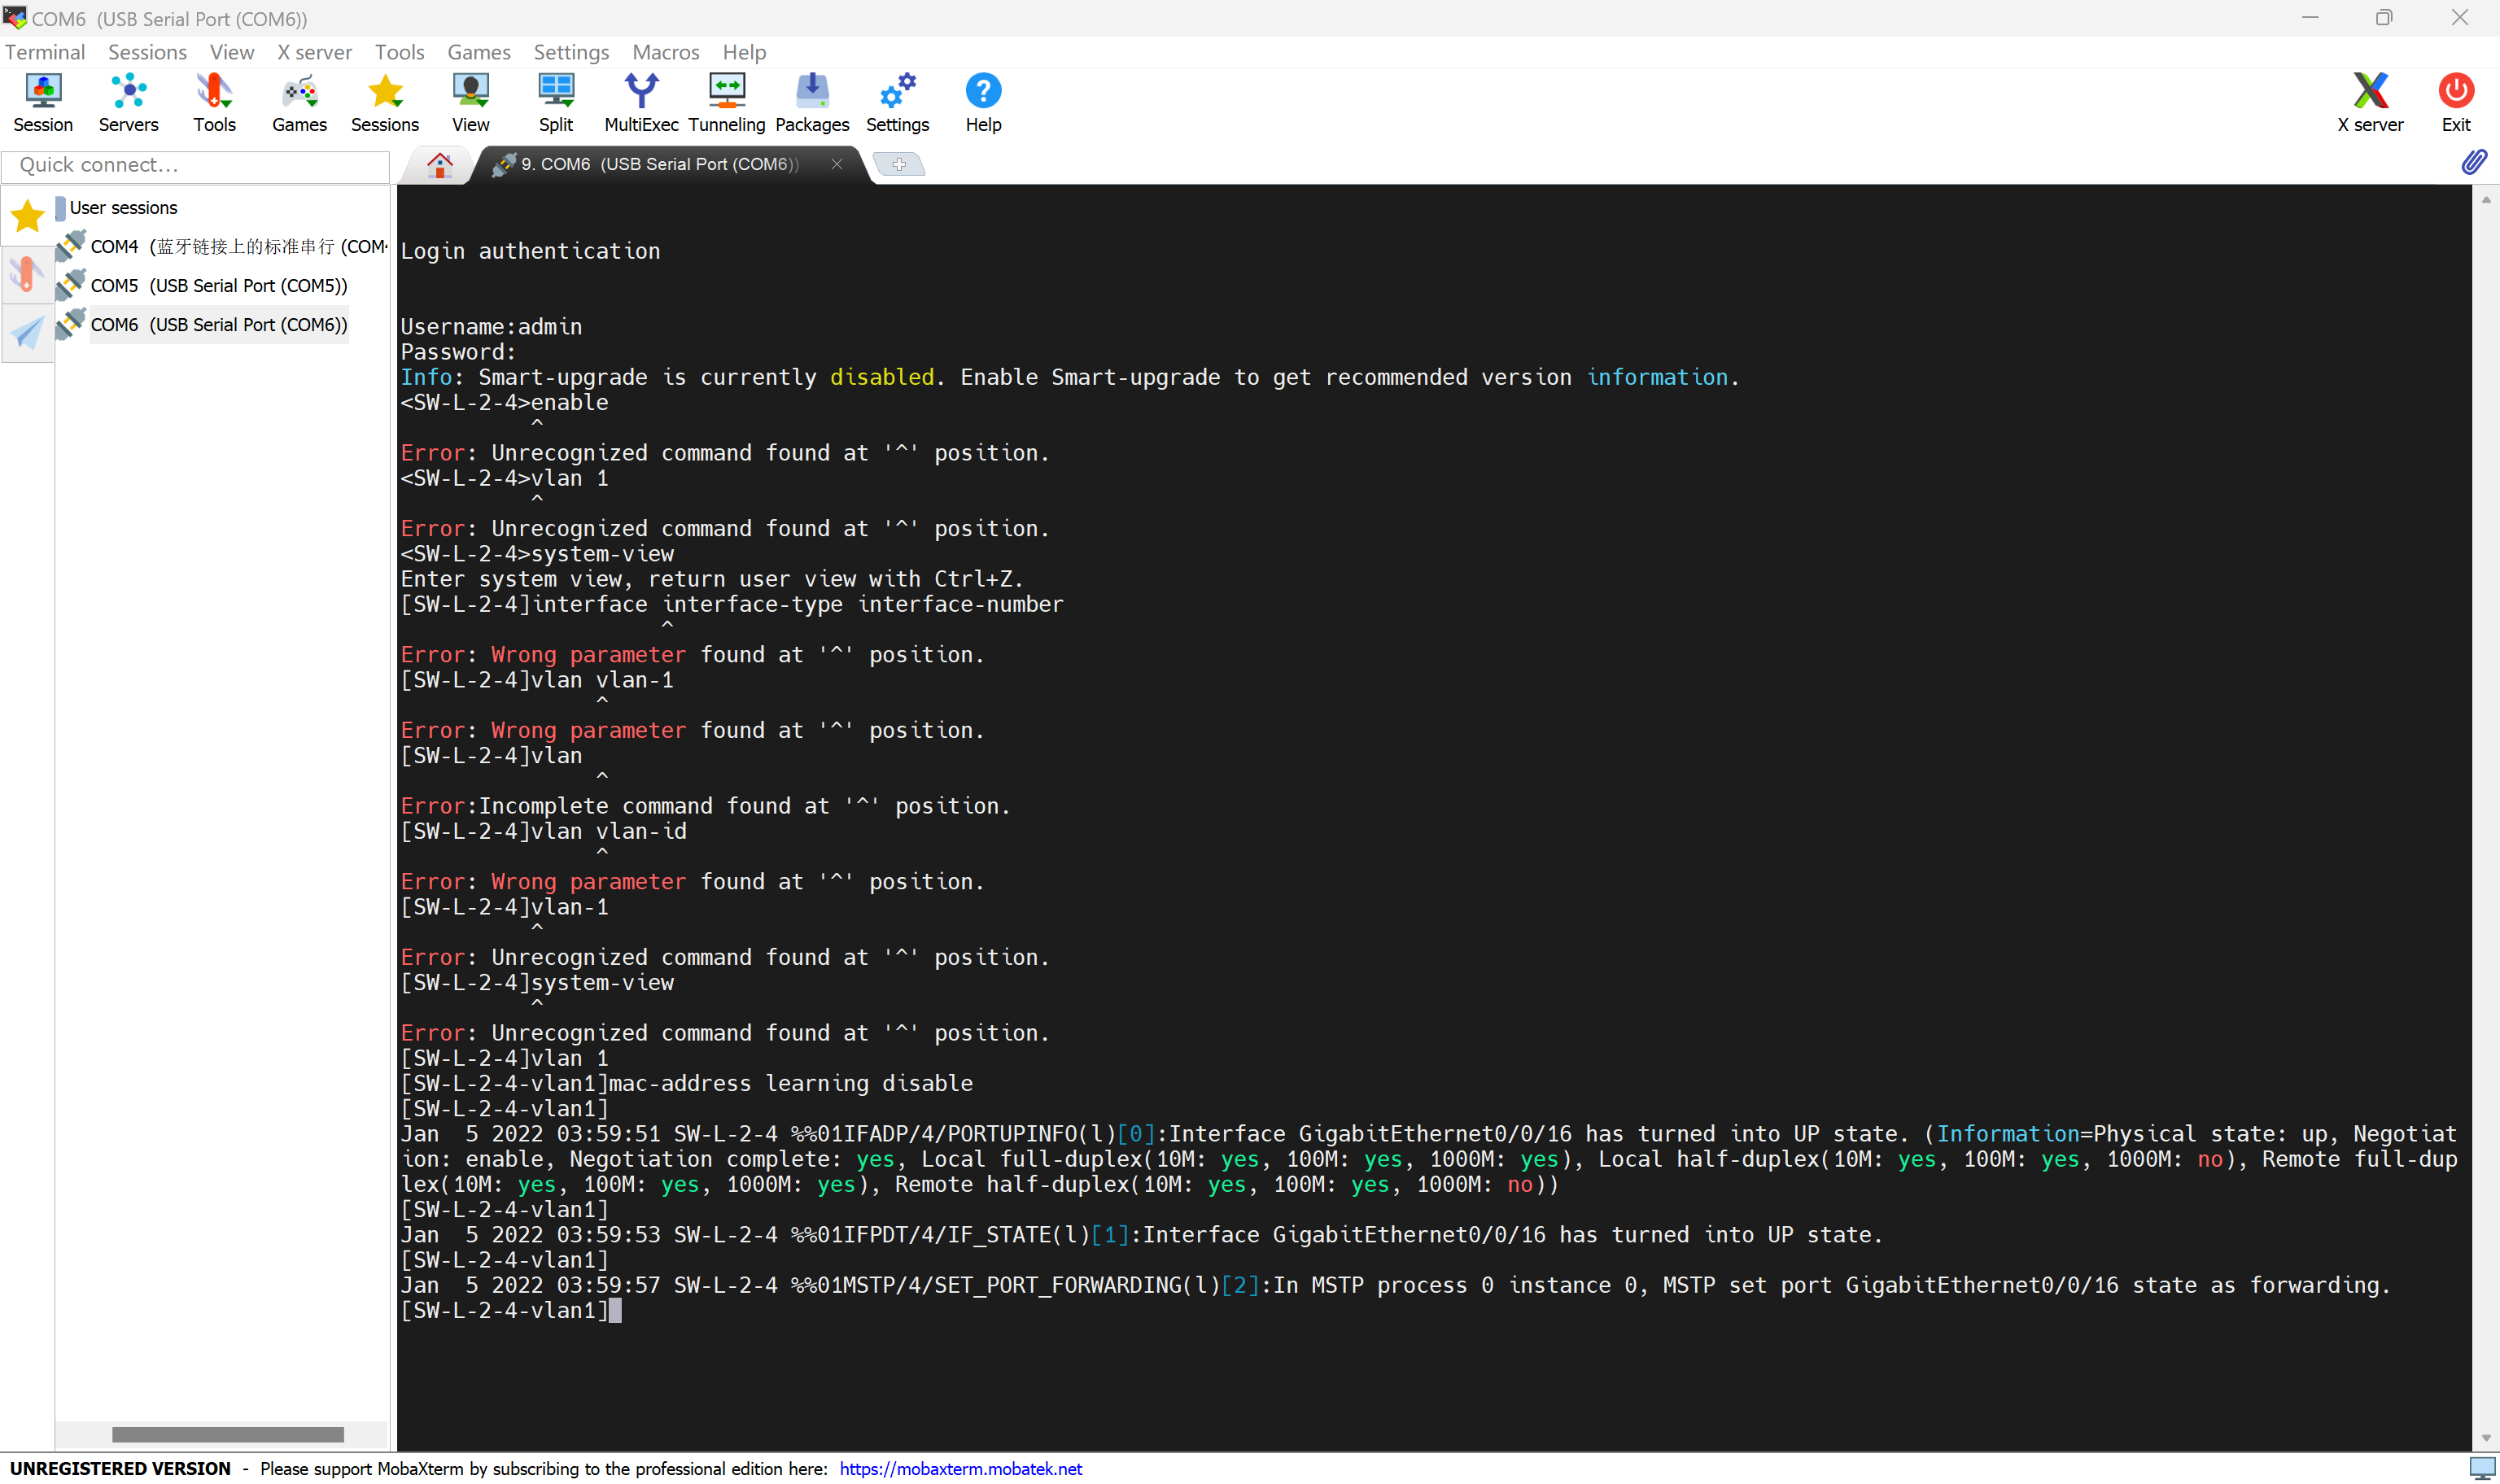
\includegraphics[width=0.5\textwidth]{2_2_images/10.png}
\end{center}
\vspace{10pt}

\subsubsection{PC间收发包}
用网线将电脑按照拓扑图连接好,然后在A上用小兵发包,目的MAC设置为B的MAC地址,在C上观察Wireshark抓包情况。
A给B发ARP包:
\begin{center}
    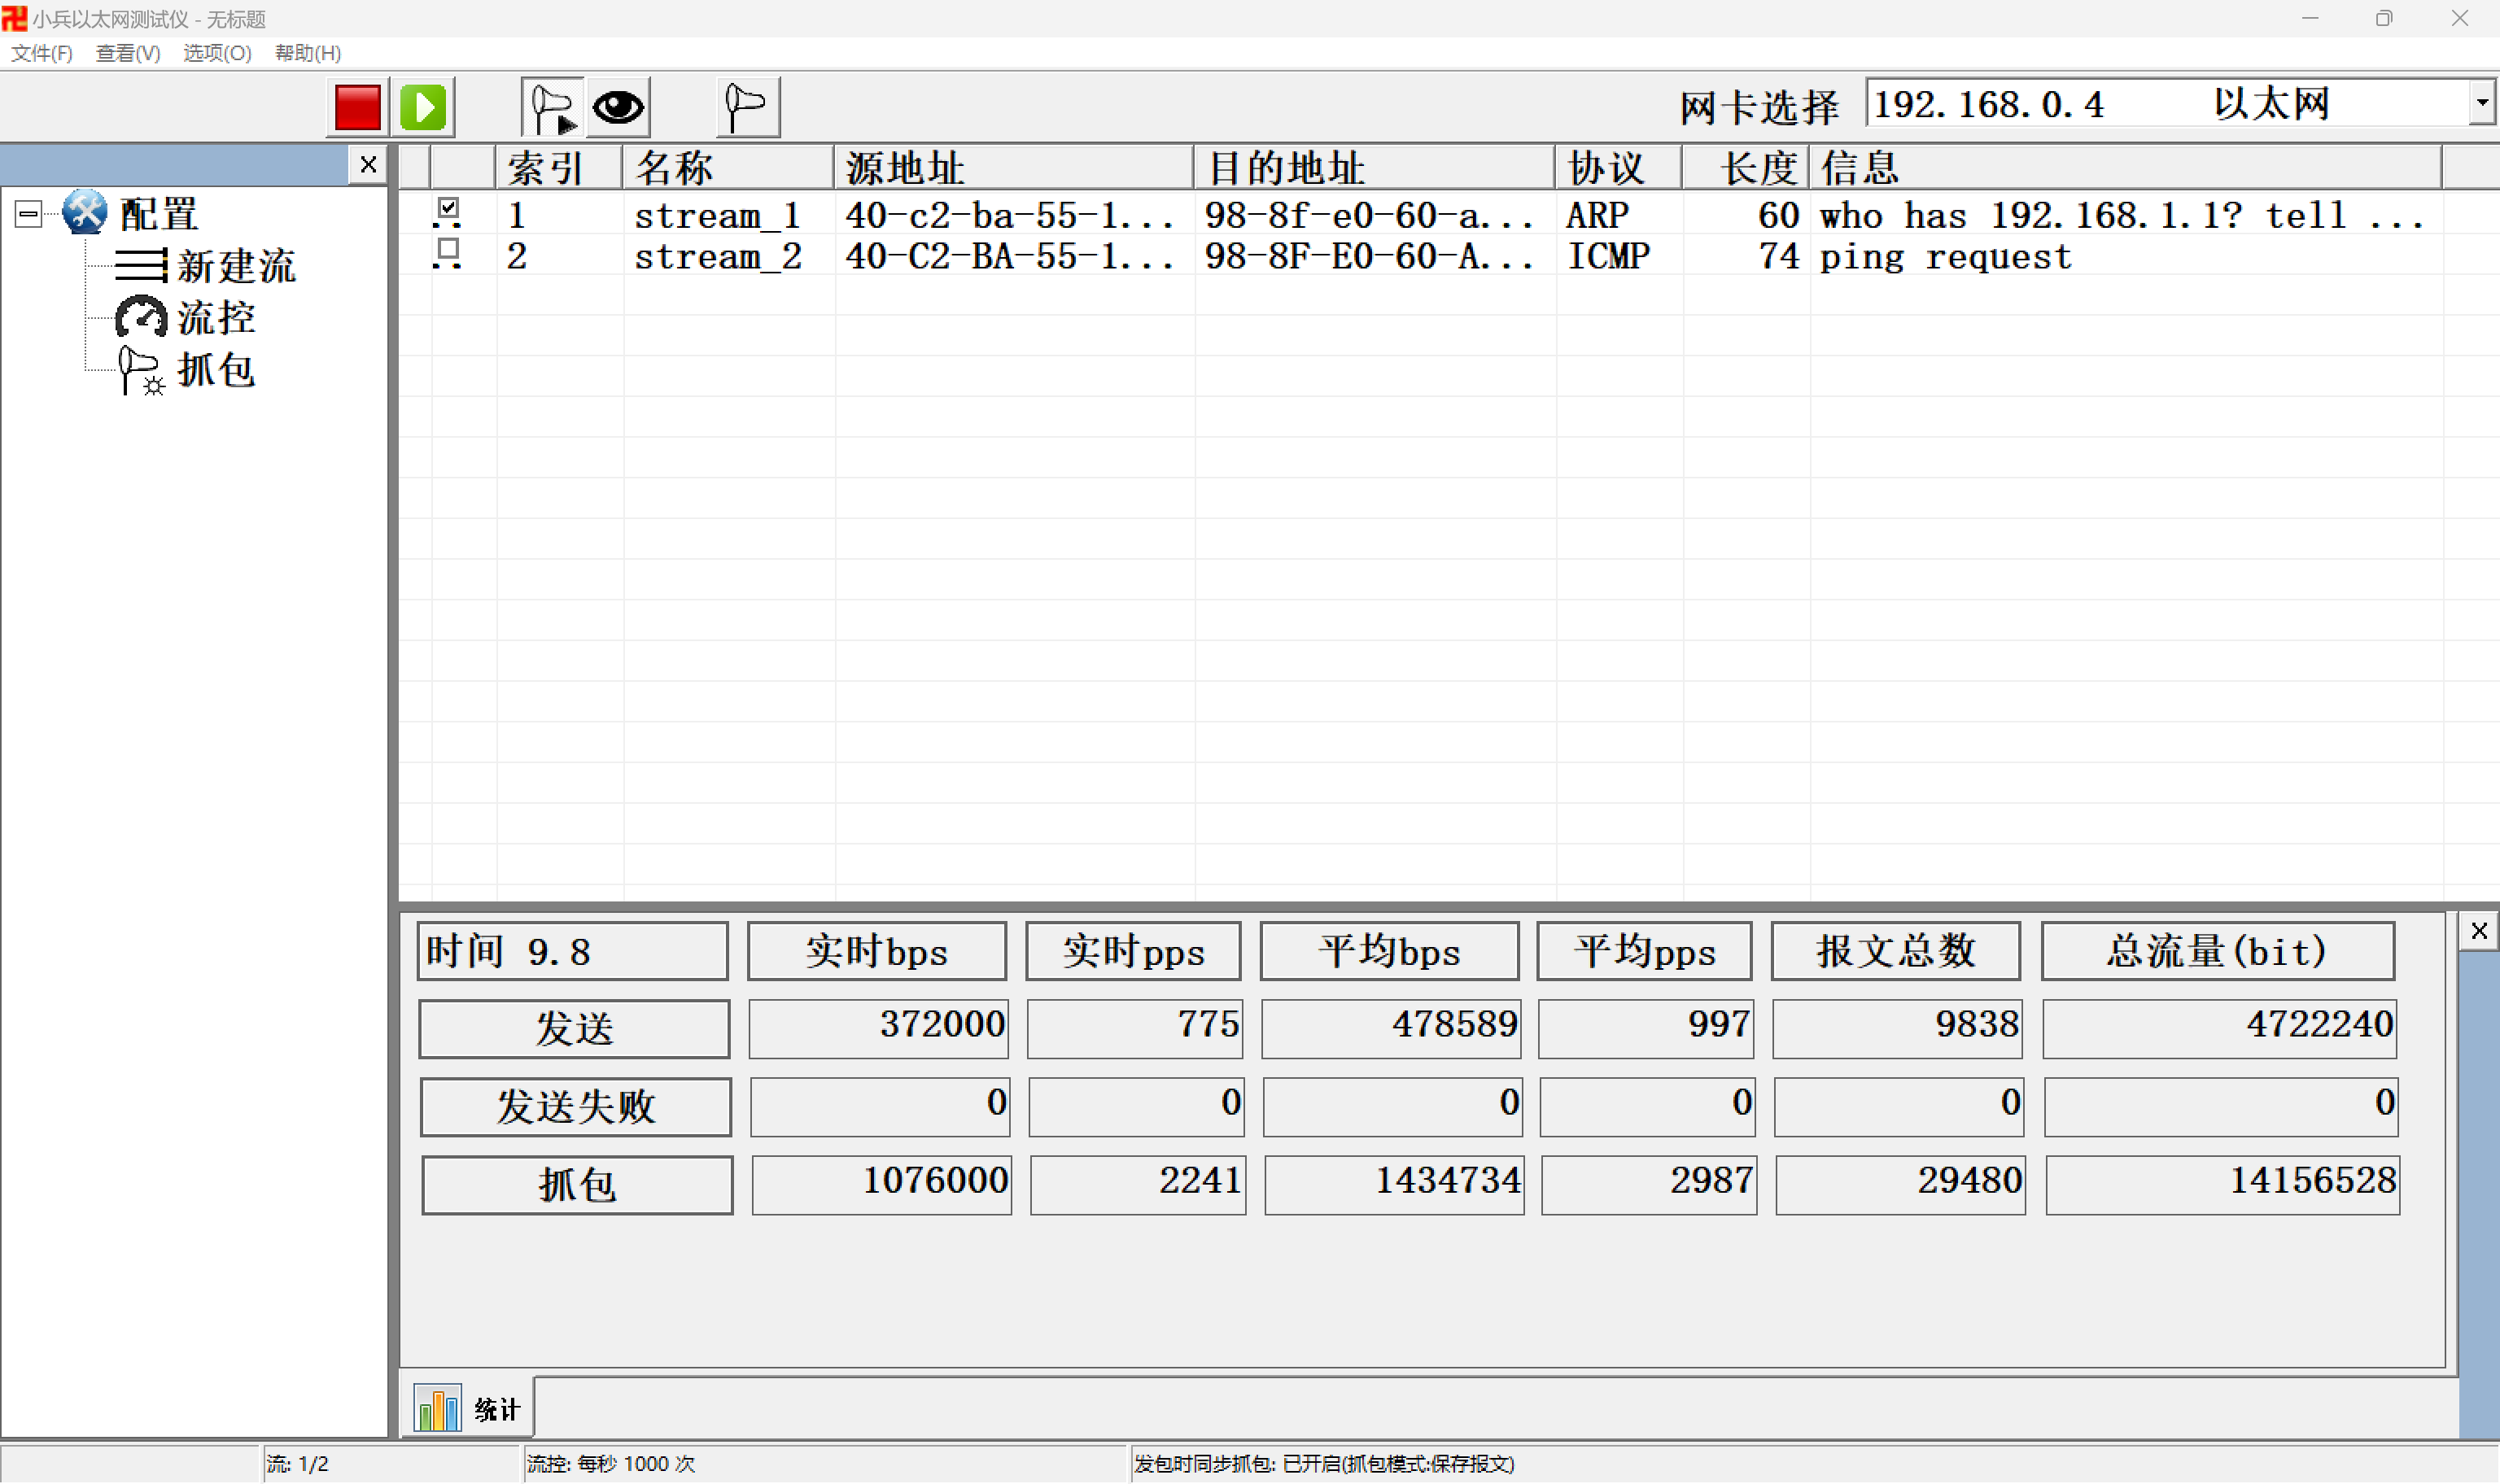
\includegraphics[width=0.5\textwidth]{2_2_images/11.png}
\end{center}
\vspace{10pt}

B收到ARP包并返回响应报文:
\begin{center}
    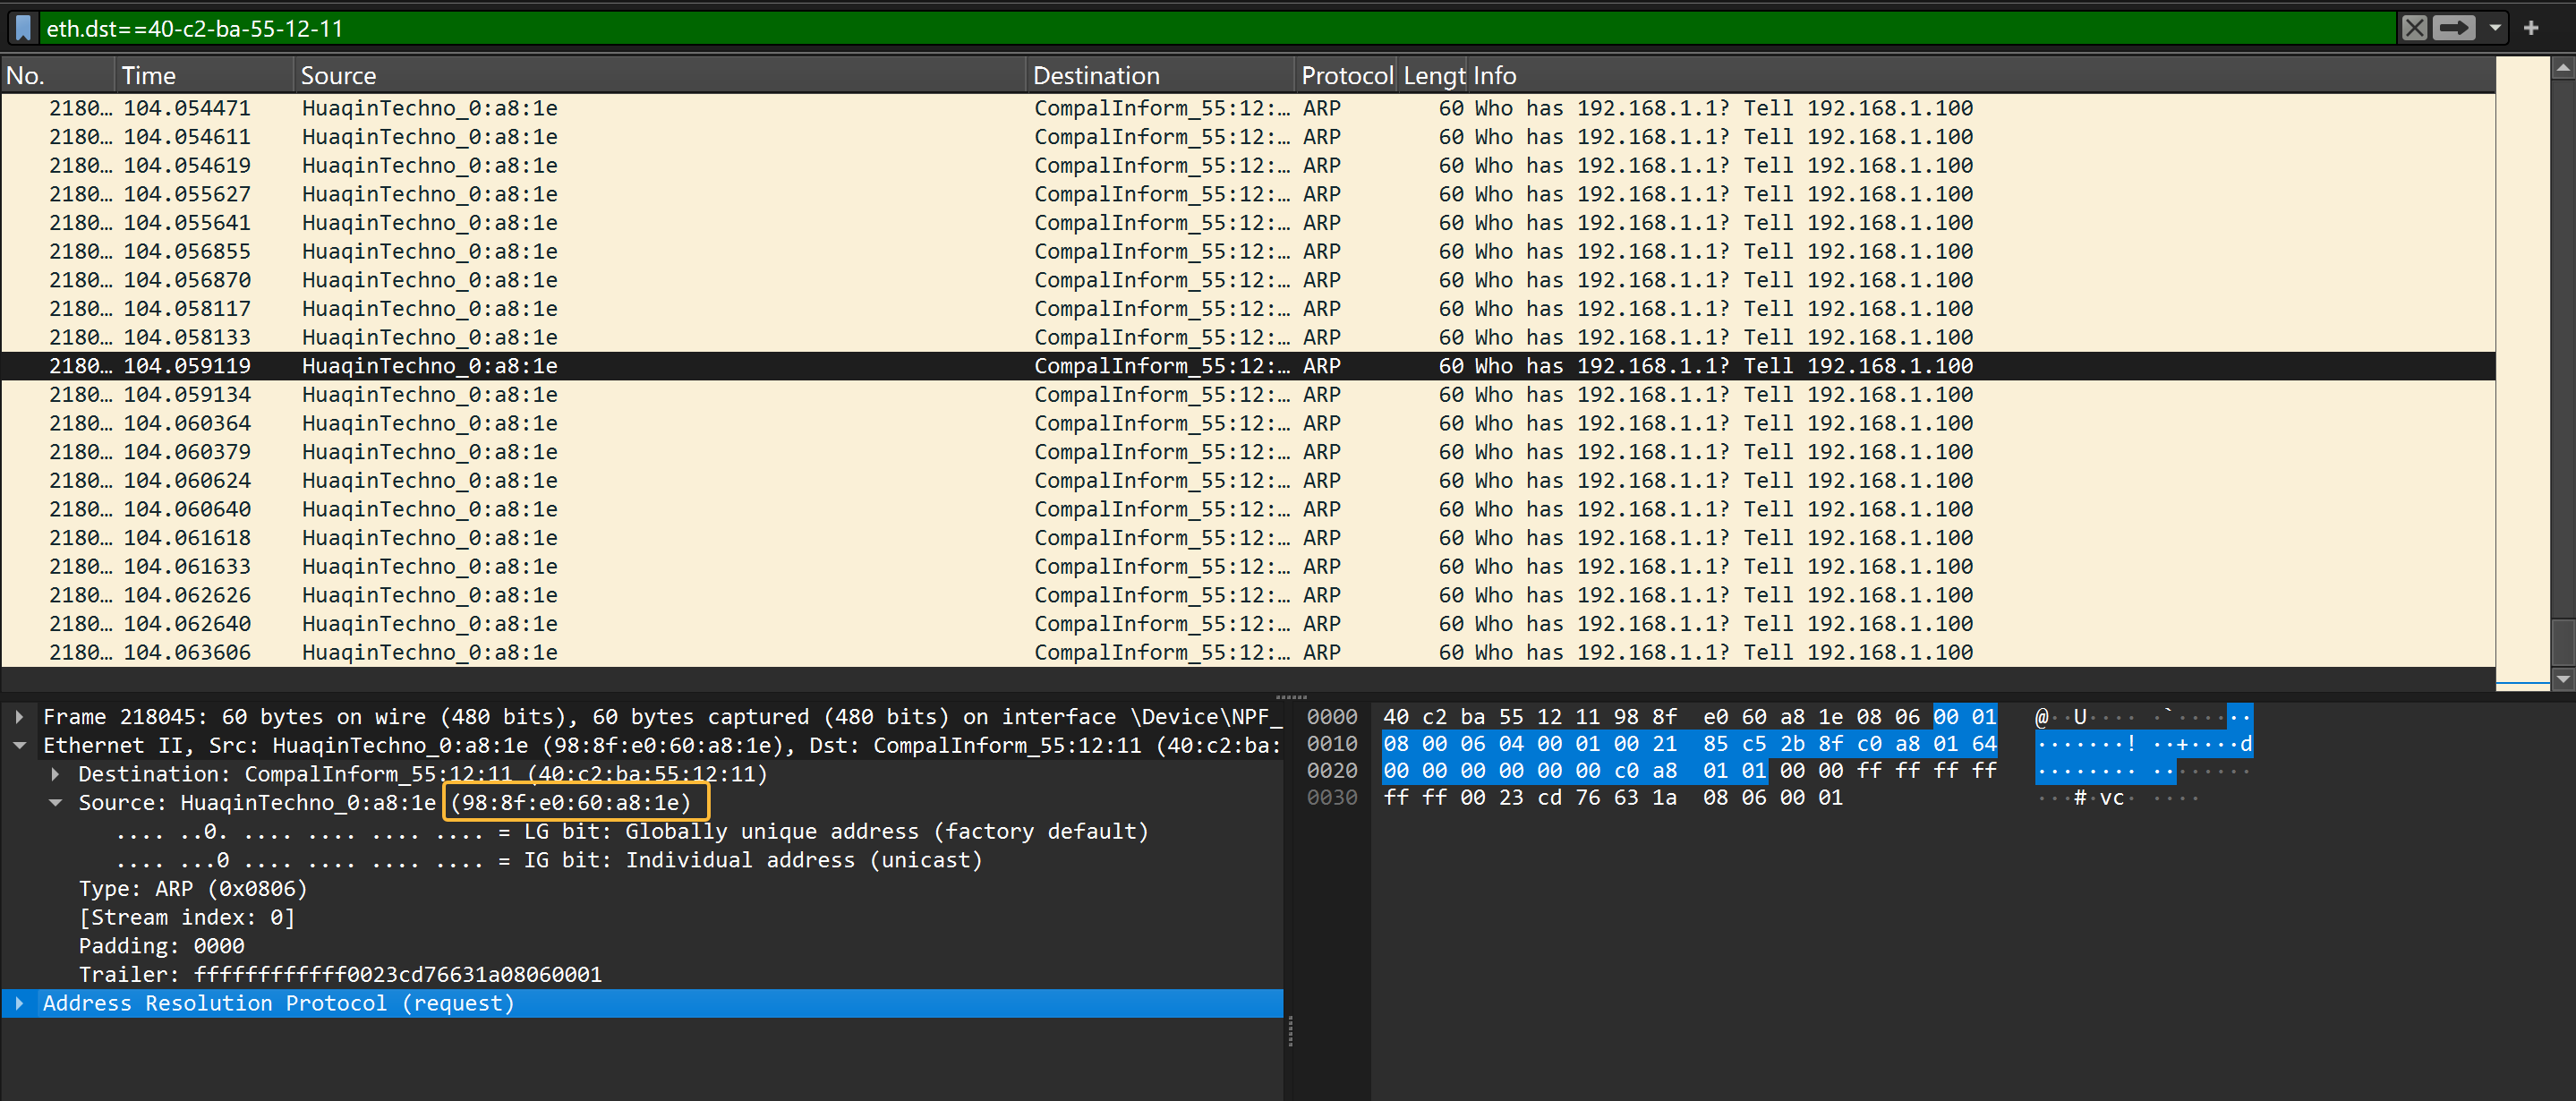
\includegraphics[width=0.5\textwidth]{2_2_images/12.png}
\end{center}
\vspace{10pt}

C收到A发出的广播报文:
\begin{center}
    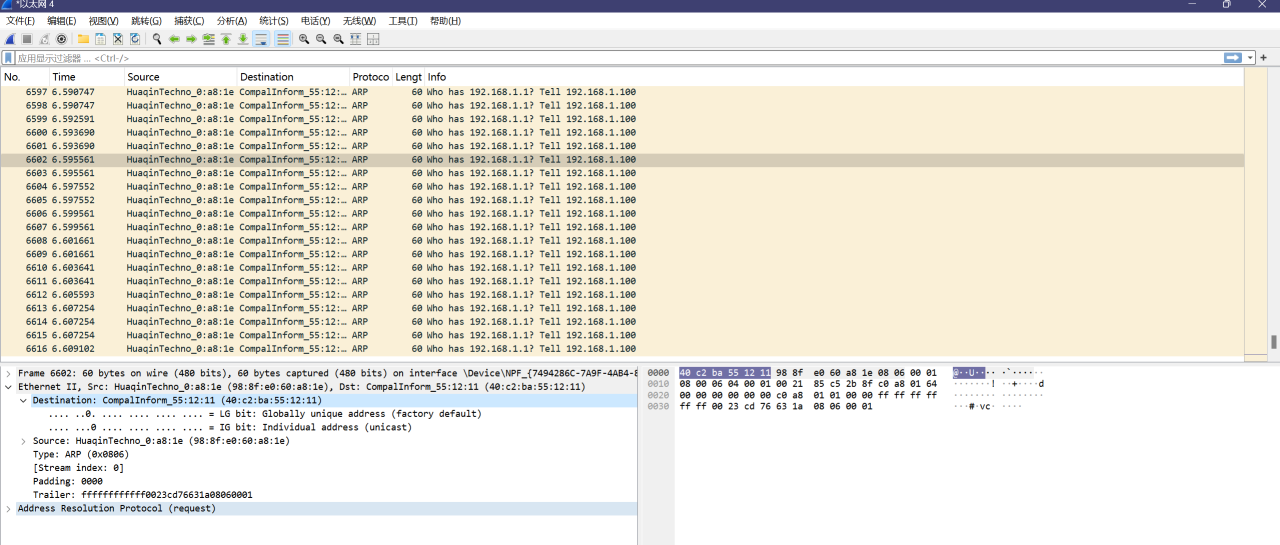
\includegraphics[width=0.5\textwidth]{2_2_images/13.png}
\end{center}
\vspace{10pt}

可以看到C电脑也收到了AB之间的信息,因为关闭了MAC自学习功能,所有的传输都是广播的。

\subsection{实验思考}
\begin{itemize}
    \item 1. PC机MAC地址是怎样分配的?保存在哪里?
    \item 答:PC机MAC地址是由网络设备商在生产时烧录的,MAC地址是全球唯一的,由IEEE统一分配,确保在网络中准确标识和定位每一个设备。存储在网卡内部的EEPROM或Flash芯片中,通过I2C或SPI接口连接。
    
    \item 2. 网卡收到其它PC的帧,怎样确定是否要继续处理?
    \item 答:会检查帧的目的MAC地址是否与自己的MAC地址匹配。如果匹配,则网卡会进一步处理这个帧;如果不匹配,网卡通常会丢弃这个帧。
\end{itemize}

\subsection{心得体会}
通过使用小兵软件进行发包实验,我们观察了不同目的MAC地址设置下的数据包传输行为,并对集线器环境下的网络通信有了更直观的理解。集线器这种方式对于所有的报文都进行广播,效率低而且可能产生冲突。




\newpage\section{实验2.4 多PC通过交换机组网}
\subsection{实验目的}
测试交换机的功能,理解交换机的工作原理。
\subsection{实验内容}
\begin{itemize}
    \item 方案:
    \item 交换机启动mac学习(因为在2.2实验中被老师关闭了)
    \item 3 PC机使用IP协议,静态配置IP地址*
    \item PC机使用有线网卡,使用网线,接入临近交换机
    \item 3 PC间互相ping,观察连通性
    \item 验收:
    \item 非混杂模式抓包
    \item 查看PC机网卡的MAC地址
    \item 查看交换机MAC学习情况,确定PC机网卡MAC是否正确学习到
    \item PC3机收到哪几台PC的ARP request, reply报文,为什么?
    \item PC1 ping PC2 时, PC3是否会收到,为什么?
\end{itemize}
\subsection{小组成员及分工}
小组共三名成员,三台PC均连到交换机上,共同完成实验,其中梁耀欣的电脑负责控制交换机的学习功能。IP配置如下:

梁耀欣: A: 192.168.0.4

李昶瑾: B: 192.168.0.3

赵露苗: C: 192.168.0.5

\subsection{实验过程与结果分析}
首先按照实验2.3的拓扑图搭建电脑和交换机结构。
\subsubsection{交换机启动MAC学习}
用console接口连接电脑,进入mobaXterm,选择对应的USB接口,输入账户密码,从用户模式切换到特权模式,进入VLAN1的配置模型,进入系统视图,选择要配置的网络接口然后启用交换机自学习功能:
输入代码:
\begin{lstlisting}
system -view
vlan 1
undo mac-address learning disable
\end{lstlisting}

命令行结果:

\vspace{10pt}
\centerline{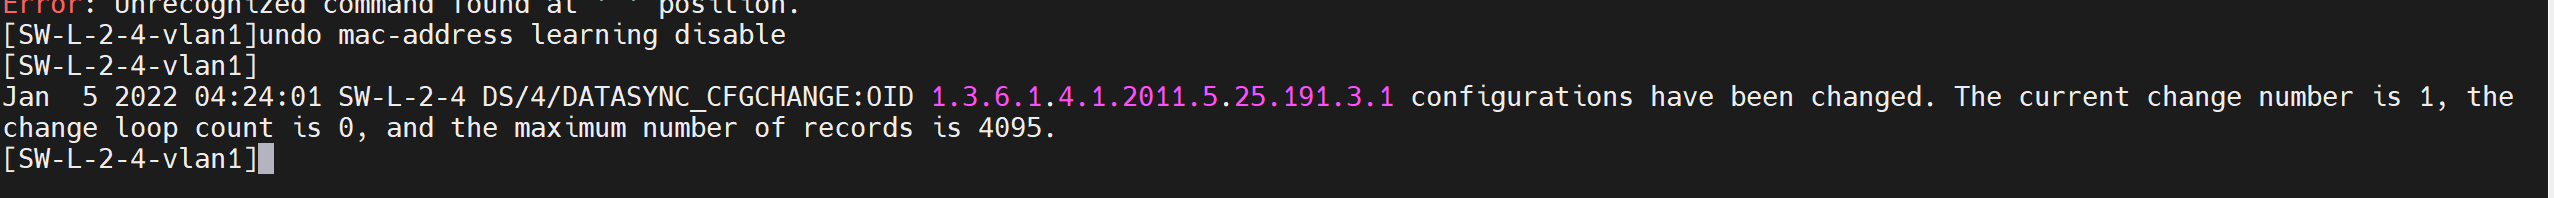
\includegraphics[width=1\textwidth]{2_4_images/1.png}}
\vspace{10pt}

\subsubsection{三台PC机静态配置IP地址}

\subsubsection{三台PC机互相ping,观察连通性}
以下是三台机器互相ping的截屏:

\vspace{10pt}
\centerline{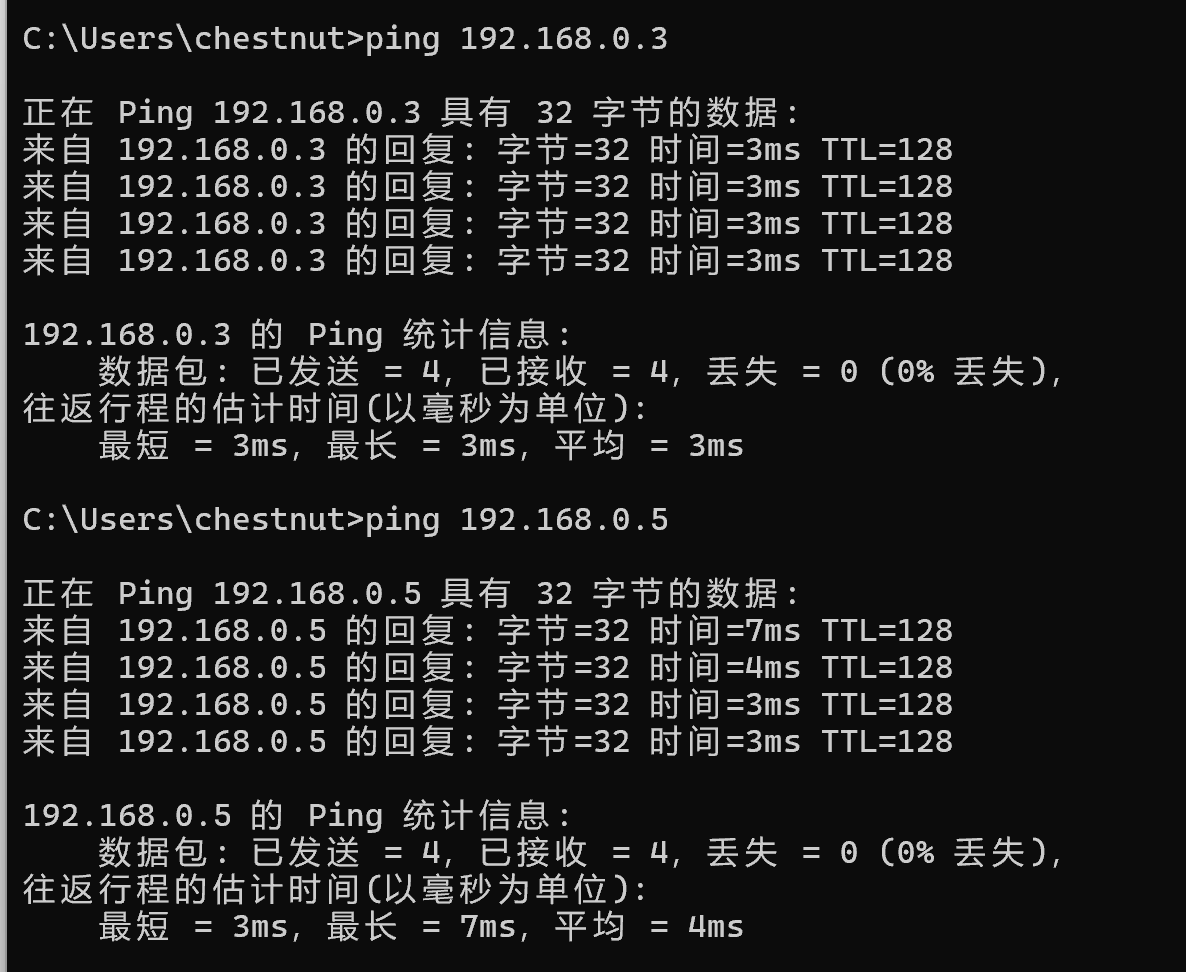
\includegraphics[width=0.5\textwidth]{2_4_images/2.png}}
\vspace{10pt}

\vspace{10pt}
\centerline{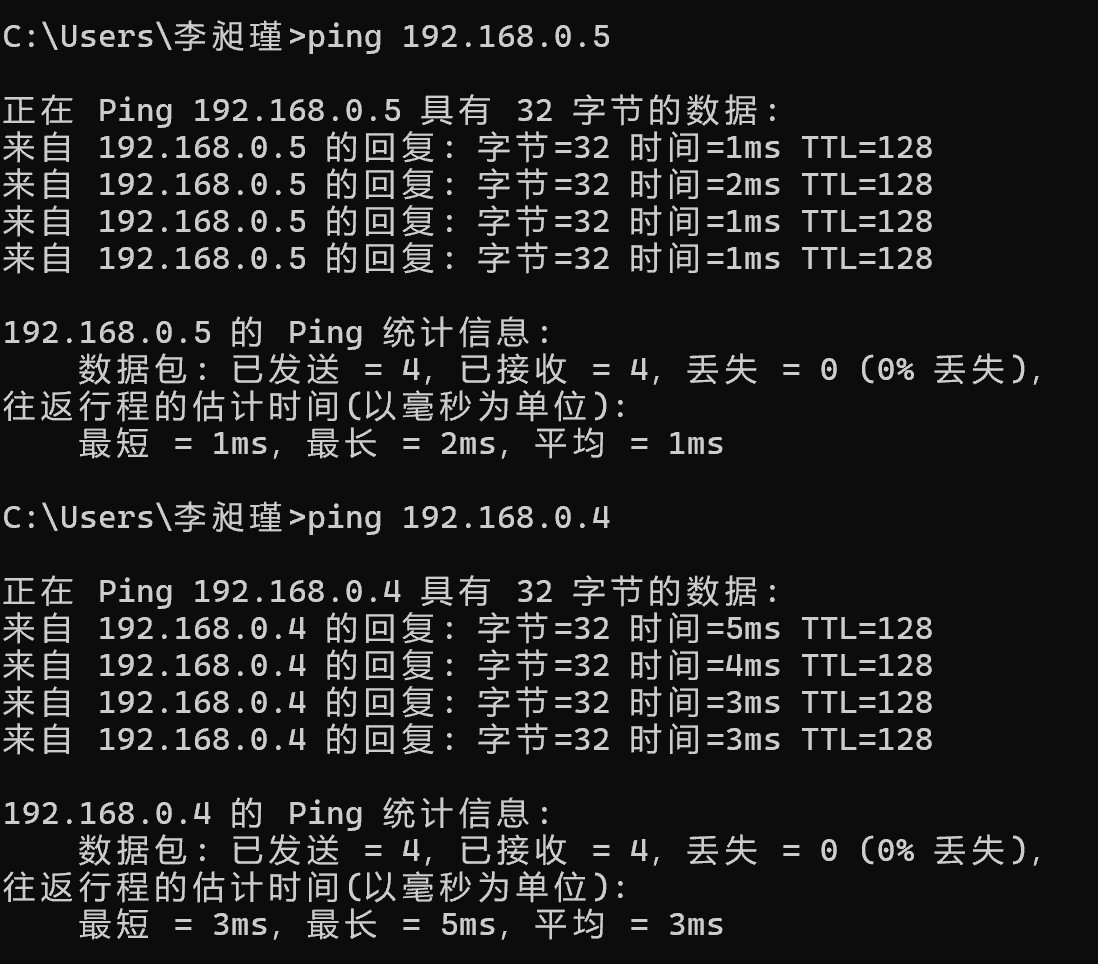
\includegraphics[width=0.5\textwidth]{2_4_images/3.png}}
\vspace{10pt}

\vspace{10pt}
\centerline{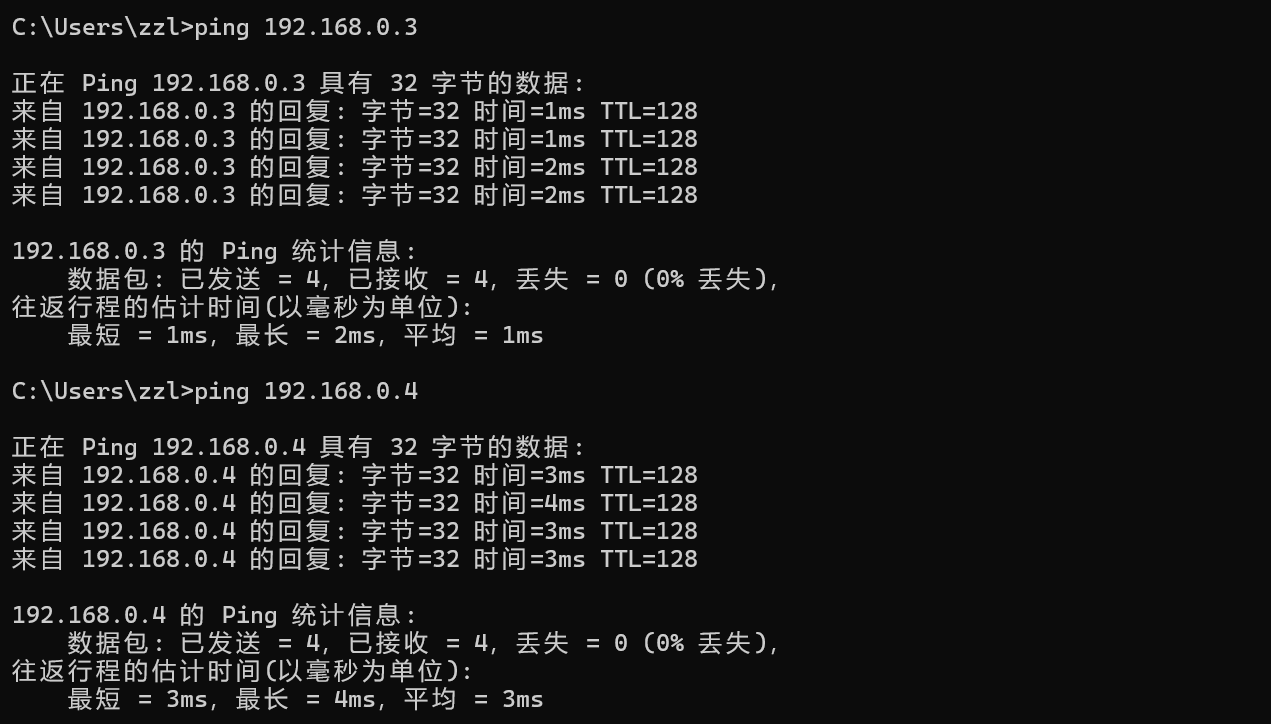
\includegraphics[width=0.5\textwidth]{2_4_images/4.png}}
\vspace{10pt}

\subsubsection{其中两台PC机ping,检验第三台能否看到}
A ping B,B收到ping请求和回复:

\vspace{10pt}
\centerline{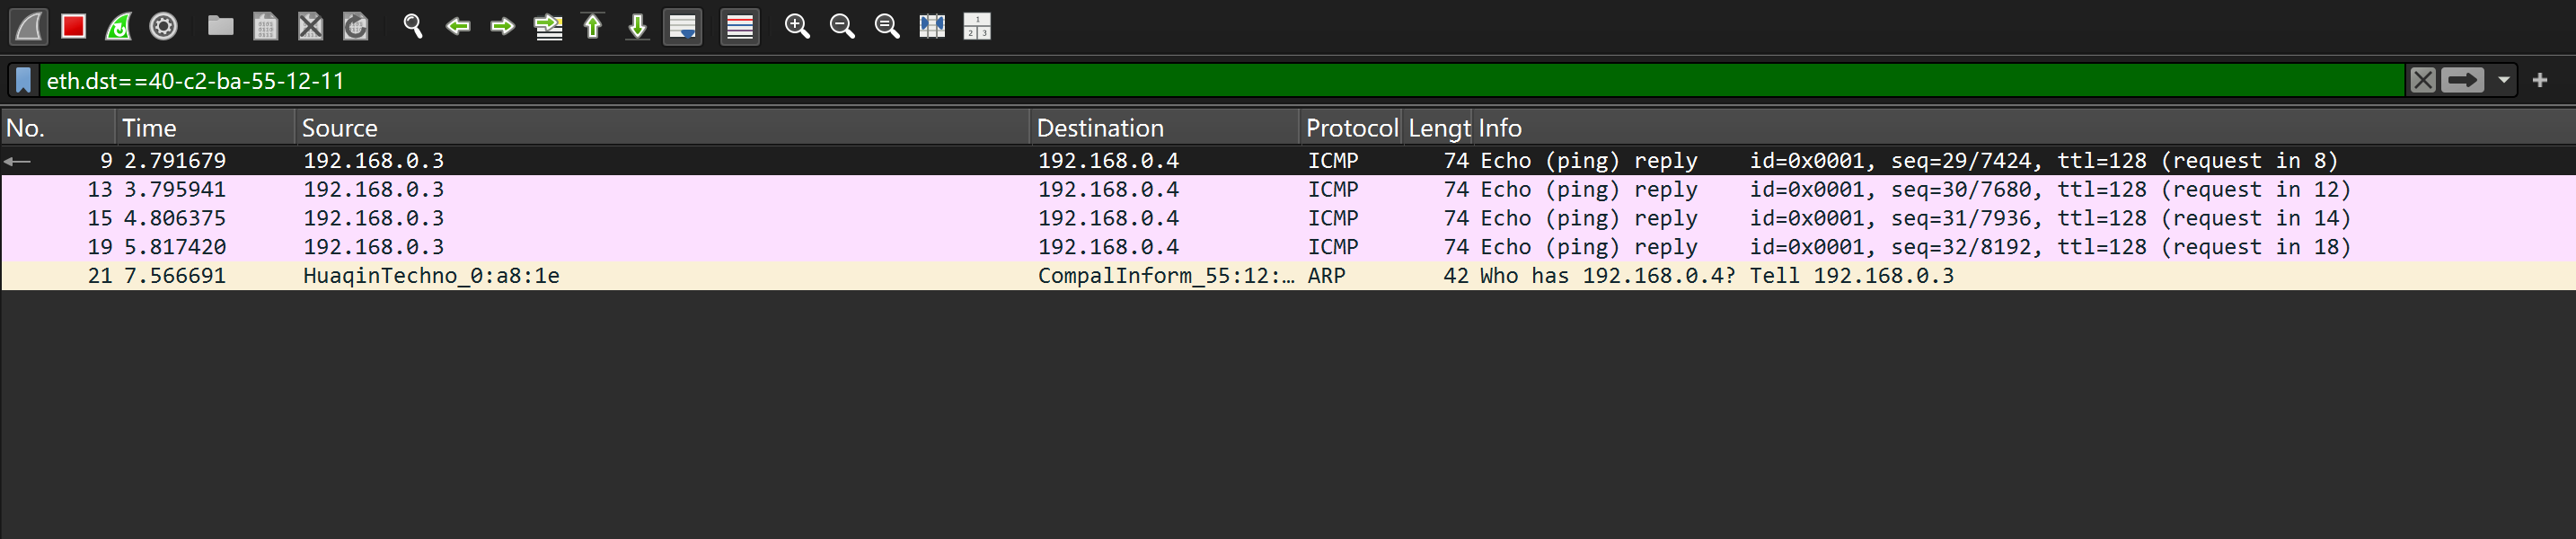
\includegraphics[width=0.5\textwidth]{2_4_images/5.png}}
\vspace{10pt}

\vspace{10pt}
\centerline{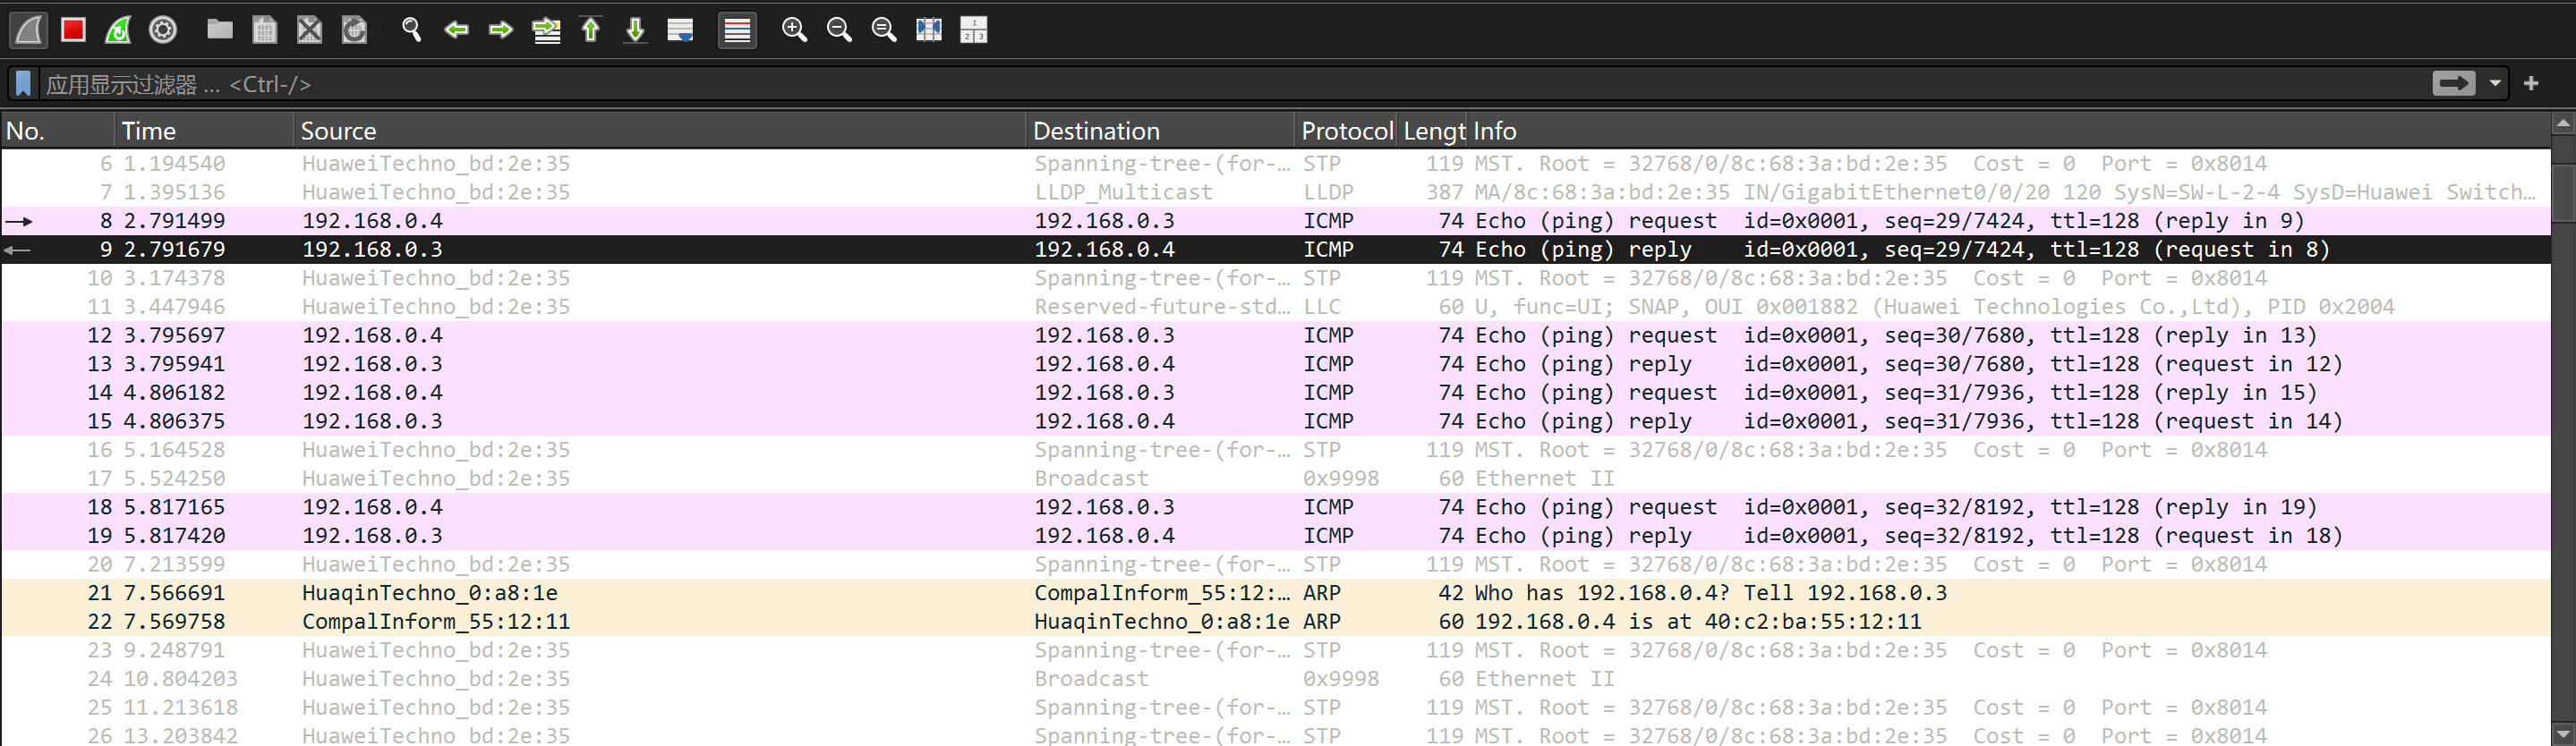
\includegraphics[width=0.5\textwidth]{2_4_images/7.png}}
\vspace{10pt}
C没收到ping请求,也没看到B的回复:

\vspace{10pt}
\centerline{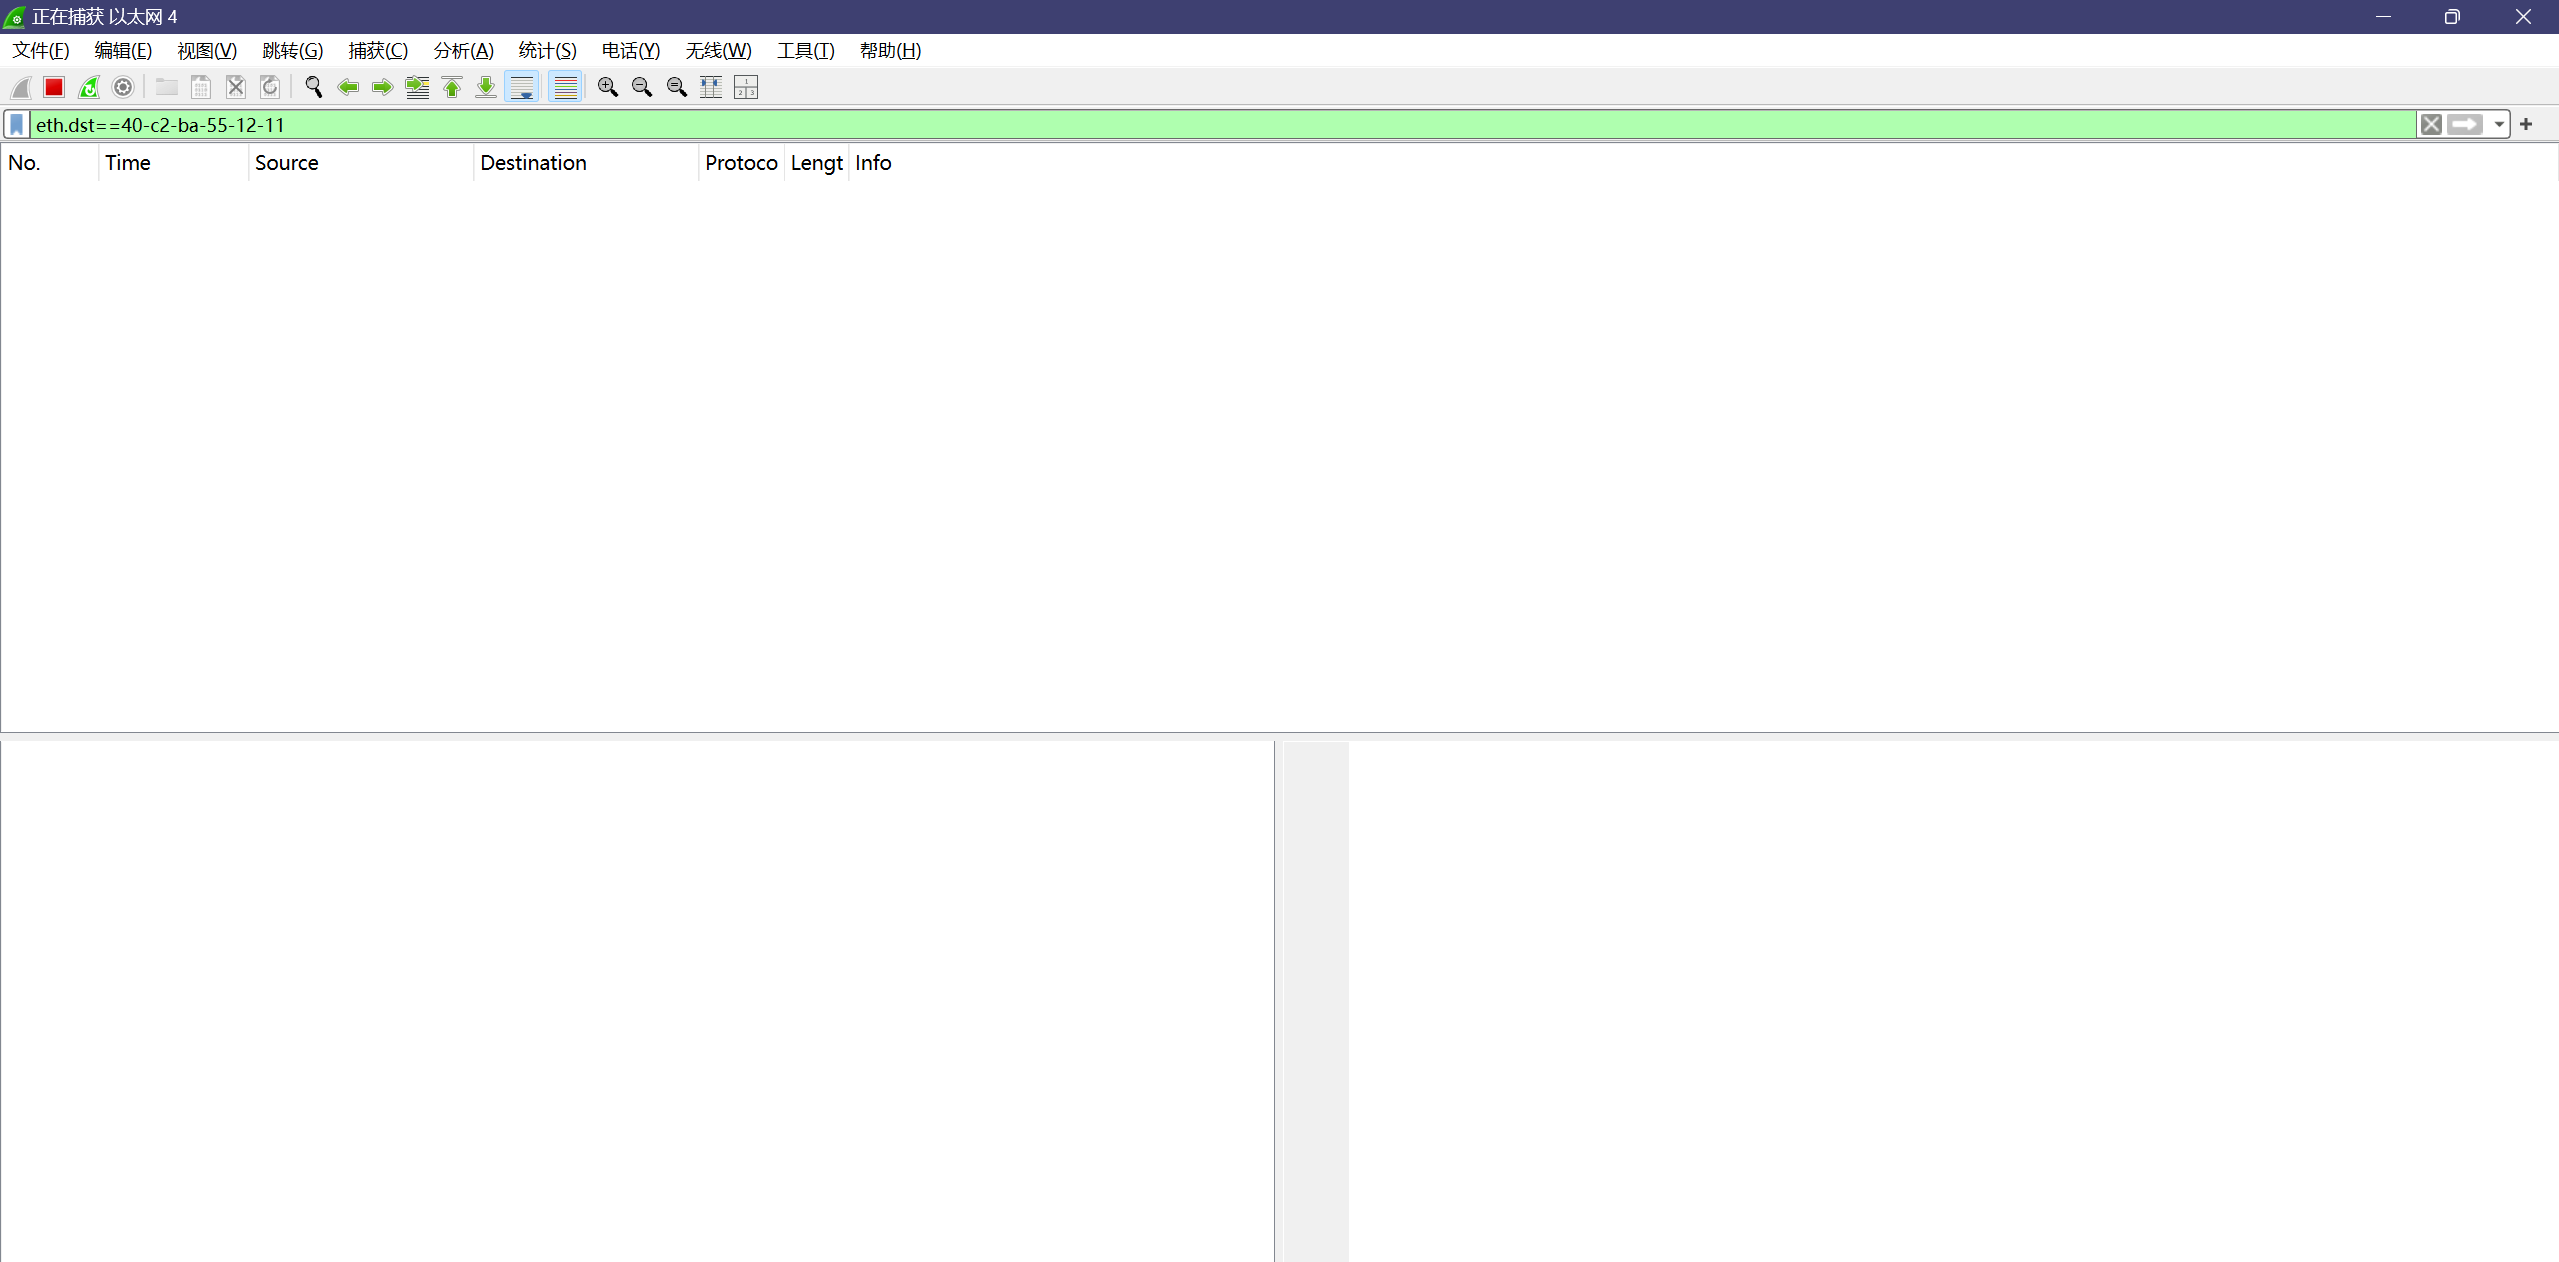
\includegraphics[width=0.5\textwidth]{2_4_images/6.png}}
\vspace{10pt}
在网络通信中,当主机A试图对主机B执行 ping 操作时,其过程如下。起初,A 会构建一个带有B的 IP 地址的 ICMP 回显请求数据包。鉴于在数据链路层通信需要目的主机的MAC地址,若A此时尚未知晓B的MAC地址,便会向网络中发送 ARP 请求以获取该信息。当B接收到此 ARP 请求后,会向A回复包含其MAC地址的响应。A 在获取到B的MAC地址后,将之前生成的 ICMP 请求封装成数据帧,随后借助交换机进行传输。交换机依据自身的MAC地址表来确定数据帧的转发路径,若B与A处于同一交换机的连接范围内,该数据帧将会被直接转发至B所连接的端口。B收到此数据帧后,会生成一个与之对应的 ICMP 回显应答数据包,同样通过交换机将其回传至A。最终,A 成功接收到来自B的应答,从而完成了一次完整的 ping 操作。
\subsection{实验思考}   
\begin{itemize}
    \item 1.mac学习会学习哪几个关键key?
    \item 会学习mac地址与对应的端口以及VLAN信息。
    \item 2.为什么学习到的mac地址会老化?不老化有什么问题?
    \item 适应网络的变化和维护MAC地址表的有效性,防止MAC资源表浪费。老化机制允许交换机删除不再使用的MAC地址,释放表项空间,以便于后续学习其他新的MAC地址。不老化可能遇到资源浪费、地址表满等问题。
\end{itemize}


\subsection{心得体会}
通过这次实验,我深刻理解了交换机的工作原理,特别是MAC学习过程和转发决策机制。我学会了如何配置静态IP地址,并通过实际操作理解了ARP协议在网络通信中的作用。此外,我还掌握了如何在非混杂模式下抓包,这对于网络故障诊断和性能分析非常有用。交换机通过学习MAC地址来优化网络流量的转发,减少不必要的广播,从而提高网络效率;交换机的MAC地址表对于网络的正确运作至关重要,它需要定期更新以反映网络中设备的变化。


\newpage\section{实验2.5 使用交换机+VLAN组网}
\subsection{实验目的}
测试VLAN的功能,理解VLAN的工作原理。
\subsection{实验内容}
\begin{itemize}
    \item 方案:
    \item 3 PC机使用IP协议,静态配置IP地址。
    \item PC机使用有线网卡,使用网线,接入临近交换机。
    \item 交换机间通过网线互联,相互连通。
    \item 研发PC1/PC2 分配VLAN1,财务PC3分配VLAN 2。
    \item PC2 变更为财务部PC,接入到Switch1上,进行实验。
    \item 验收:
    \item 当前组网实验:研发体系PC可以互通,与财务体系PC不能互通
    \item 查看交换机上MAC学习情况: display mac-address,学习到的macaddress/接口/VLAN情况
\end{itemize}
\subsection{小组成员及分工}
小组共三名成员,三台PC均连到交换机上,共同完成实验,其中我的电脑负责控制交换机3的学习功能。

本次实验的IP:
\begin{itemize}
    \item 192.168.0.3:98-8F-E0-60-A8-1E
    \item 192.168.0.4:40-C2-BA-55-12-11
    \item 192.168.0.7:C8-4D-44-29-48-88
\end{itemize}

\subsection{实验过程与结果分析}
\subsubsection{按照拓扑图搭建交换机}
\vspace{10pt}
\centerline{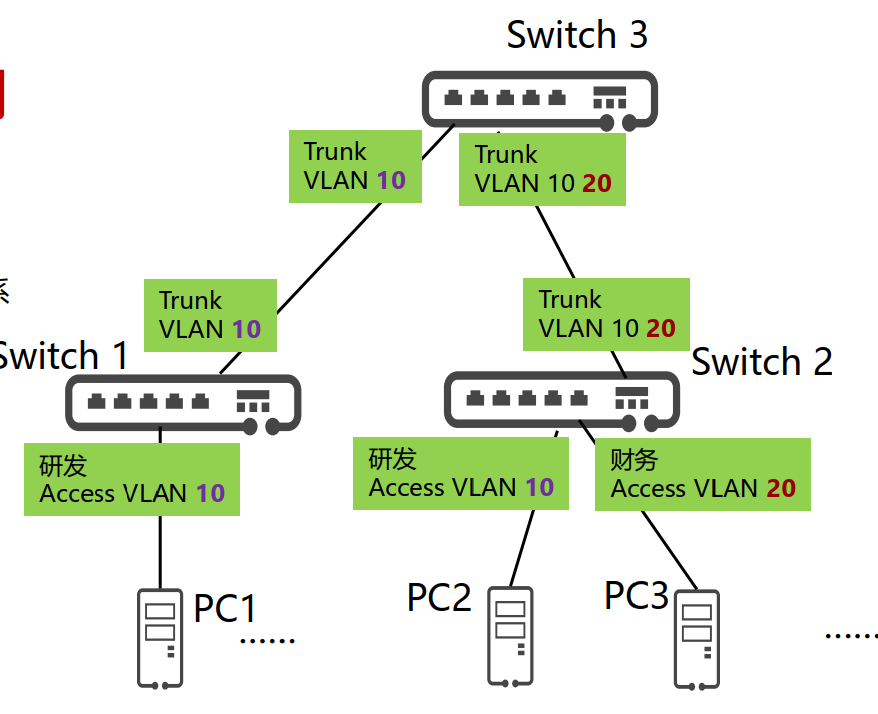
\includegraphics[width=0.5\textwidth]{2_5_images/1.png}}
\vspace{10pt}
根据上图所示的拓扑图进行交换机的设置,其中本机负责控制switch3的功能,设置如下:
\begin{lstlisting}
vlan 1
interface gigabitethernet 0/0/14
port link-type trunk
portTrunkallow-pass vlan 10
vlan 2
interface gigabitethernet 0/0/20
port link-type trunk
portTrunkallow-pass vlan 2
\end{lstlisting}
设置完成后进行ping实验,结果如下:
\begin{itemize}
    \item PC3无法ping通PC1和PC2,因为不属于同一个部门:
    \item \vspace{10pt}
    \centerline{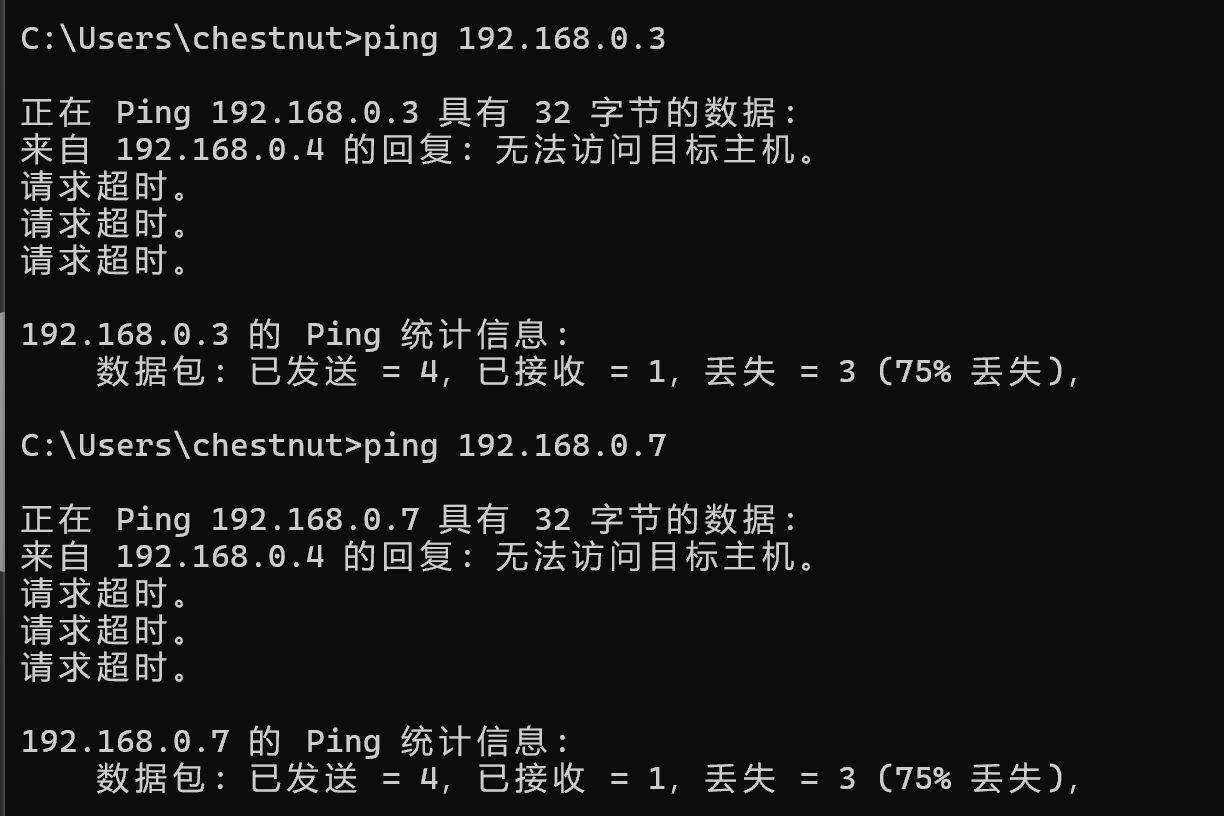
\includegraphics[width=0.5\textwidth]{2_5_images/2.png}}
    \vspace{10pt}
    \item PC2可以ping通PC1,ping不通PC3:
    \item \vspace{10pt}
    \centerline{\includegraphics[width=0.5\textwidth]{2_5_images/3.png}}
    \vspace{10pt}
    \item PC1可以ping通PC2,不可以ping通PC3:
    \item \vspace{10pt}
    \centerline{\includegraphics[width=0.8\textwidth]{2_5_images/4.png}}
    \vspace{10pt}
\end{itemize}

switch1显示学习到的MAC地址:

\vspace{10pt}
\centerline{\includegraphics[width=0.8\textwidth]{2_5_images/5.png}}
\vspace{10pt}
switch2显示学习到的MAC地址:

\vspace{10pt}
\centerline{\includegraphics[width=0.8\textwidth]{2_5_images/6.png}}
\vspace{10pt}
switch3显示学习到的MAC地址:

\vspace{10pt}
\centerline{\includegraphics[width=0.8\textwidth]{2_5_images/7.png}}
\vspace{10pt}

\subsubsection{改变PC2后重新搭建}
变更pc2到财务部后pc3的ping:

\vspace{10pt}
\centerline{\includegraphics[width=0.5\textwidth]{2_5_images/9.png}}
\vspace{10pt}
PC2ping通PC3,不通PC1:

\vspace{10pt}
\centerline{\includegraphics[width=0.5\textwidth]{2_5_images/10.png}}
\vspace{10pt}
PC1不通PC2,PC3:

\vspace{10pt}
\centerline{\includegraphics[width=0.8\textwidth]{2_5_images/11.png}}
\vspace{10pt}

\subsubsection{实验错误纠正}
在对Switch1进行交换机配置调整的过程中,仅仅对 Access 部分的配置做了修改,却疏忽了Trunk部分的配置更改。由于未对Trunk进行正确的配置设定,使得 PC2 发出的 ping 数据包无法按照预期的路径,即从交换机 1 顺利传输至交换机 3 进而抵达 PC3,最终导致了 ping 不通的结果出现。

\vspace{10pt}
\centerline{\includegraphics[width=0.5\textwidth]{2_5_images/8.png}}
\vspace{10pt}

\subsection{实验思考}
\begin{itemize}
    \item 1. Access/Trunk 两种 Link Type 的差别
    \item 答:Access端口只属于一个VLAN,发送和接收的数据帧不带VLAN标签,当数据帧进入Access端口时,交换机会为数据帧打上相应的VLAN标签。Trunk端口可以允许多个VLAN的数据帧通过,发送和接收的数据帧通常带有VLAN标签。Trunk端口会根据允许通过的VLAN列表来处理数据帧。
    
    \item 2. VLAN 与物理接口的关系
    \item 答:物理接口可以被配置为属于某个VLAN,从而实现逻辑上的网络隔离。
\end{itemize}

\subsection{心得体会}
实验成功地验证了 VLAN 的隔离功能,实现了研发体系(PC1 和 PC2 初始状态)与财务体系(PC3)之间的网络隔离,即不同 VLAN 内的主机在未经过特定路由配置的情况下无法直接互通,符合 VLAN 的设计初衷,有效达到了测试 VLAN 功能的实验目的。同时,通过实验过程中的配置操作和结果分析,小组成员对 VLAN 的工作原理有了更为直观和深刻的理解,进一步深化了对网络分层和虚拟局域网概念的认知。




\newpage\section{实验3 使用L2交换机+L3交换机组网}
\subsection{实验目的}
测试VLAN的功能,理解VLAN的工作原理。
\subsection{实验内容}
\begin{itemize}
    \item 方案:
    \item 3 PC机使用IP协议,DHCP动态分配IP地址。
    \item PC机使用有线网卡,使用网线,接入临近L2交换机。
    \item L2交换机间通过L3交换机互联。
    \item L3交换机配置VLANIF,做PC机网关,并启用DHCP server为PC机分配地址。
    \item 验收:
    \item PC机可以获取IP地址。抓包分析DHCP交互过程。
    \item PC机可以互ping。
    \item 抓包分析PC机收到的数据包与实验3时有何差异?
    \item 查看路由器上路由情况:display ip routing-table。
\end{itemize}
\subsection{小组成员及分工}
小组共三名成员,其中zlm负责交换机1,PC1;lcj负责交换机2,PC2;lyx(本人)负责交换机3,PC3。
\subsection{实验过程与结果分析}
本人负责switch3的配置,输入下面的命令,创建对应的VLAN以及分配动态IP地址:
\begin{lstlisting}
vlan 1
vlan 2
dhcp enable
interface GigabitEthernet 0/0/2
port link-type trunk
portTrunkallow-pass vlan 1
interface GigabitEthernet 0/0/10
port link-type trunk
portTrunkallow-pass vlan 10 20
interface Vlanif 1
ip address 192.168.102.1 24
dhcp select interface
dhcp server dns-list 1.2.4.8
interface Vlanif 2
ip address 192.168.103.1 24
dhcp select interface
dhcp server dns-list 1.2.4.8
\end{lstlisting}
三台机器配置完vlan的图示如下:

switch1:

\vspace{10pt}
\centerline{\includegraphics[width=0.5\textwidth]{3_1_images/1.png}}
\vspace{10pt}
switch2:

\vspace{10pt}
\centerline{\includegraphics[width=0.5\textwidth]{3_1_images/2.png}}
\vspace{10pt}
switch3:

\vspace{10pt}
\centerline{\includegraphics[width=0.5\textwidth]{3_1_images/3.png}}
\vspace{10pt}

\subsubsection{抓包分析DHCP交互过程}
获取switch3给分配的动态IP地址,抓DHCP包:
PC1:

\vspace{10pt}
\centerline{\includegraphics[width=0.5\textwidth]{3_1_images/4.png}}
\vspace{10pt}
PC2:

\vspace{10pt}
\centerline{\includegraphics[width=0.5\textwidth]{3_1_images/5.png}}
\vspace{10pt}
PC3:

\vspace{10pt}
\centerline{\includegraphics[width=0.5\textwidth]{3_1_images/6.png}}
\vspace{10pt}

可以观察到DHCP的四个包均被抓到,其中
\begin{itemize}
\item DHCPDISCOVER:PC发送的DHCP请求包,用于获取IP地址。
\item DHCPOFFER:PC接收的DHCP响应包,用于告知PC可以获取IP地址。
\item DHCPREQUEST:PC发送的DHCP请求包,用于确认获取IP地址。
\item DHCPACK:PC接收的DHCP响应包,用于告知PC已经获取到IP地址。
\end{itemize}


其中DHCP报文详细信息如下:

\vspace{10pt}
\centerline{\includegraphics[width=0.5\textwidth]{3_1_images/6_1.png}}
\vspace{10pt}

该报文总长度为342字节,捕获长度与之相同。报文的到达时间为2024年11月28日09:06:55.673380000(本地标准时间)。在网络接口方面,其接口ID为0,设备标识为NP\_F6A1A31B-847F-4F5D-8147-AA0B6660,封装类型为Ethernet。

从Ethernet II层来看,源MAC地址是CompalInfo\_55:12:11,目的MAC地址是广播地址,类型为IPv4。在IPv4层,源IP地址为0.0.0.0,目的IP地址为255.255.255.255,协议为UDP,并且包含了版本、首部长度、区分服务字段等详细信息。UDP层的源端口为68,目的端口为67。

报文属于DHCP Discover类型,事务ID为0x168cd0e3,客户端硬件地址为40:c2:ba:55:12:11。报文详细列出了各层信息,包括时间戳、MAC地址、IP地址、端口号以及DHCP选项等,表明客户端正在寻找网络中的DHCP服务器。

\subsubsection{PC间互相ping的图片}
PC1 ping PC2和PC3:

\vspace{10pt}
\centerline{\includegraphics[width=0.5\textwidth]{3_1_images/7.png}}
\vspace{10pt}
PC2 ping PC1和PC3:

\vspace{10pt}
\centerline{\includegraphics[width=0.5\textwidth]{3_1_images/8.png}}
\vspace{10pt}
PC3 ping PC1和PC2:

\vspace{10pt}
\centerline{\includegraphics[width=0.5\textwidth]{3_1_images/9.png}}
\vspace{10pt}

\subsubsection{查看路由器上路由情况}
display ip routing-table
按照switch1.2.3的顺序贴上三个路由的图:

\vspace{10pt}
\centerline{\includegraphics[width=0.5\textwidth]{3_1_images/10.png}}
\vspace{10pt}

\vspace{10pt}
\centerline{\includegraphics[width=0.5\textwidth]{3_1_images/11.png}}
\vspace{10pt}

\vspace{10pt}
\centerline{\includegraphics[width=0.5\textwidth]{3_1_images/12.png}}
\vspace{10pt}

\subsubsection{查看VLANIF接口的状态信息、配置信息和统计信息}
display interface vlanif 1

配置信息如下:

\vspace{10pt}
\centerline{\includegraphics[width=0.5\textwidth]{3_1_images/13.png}}
\vspace{10pt}

\vspace{10pt}
\centerline{\includegraphics[width=0.5\textwidth]{3_1_images/14.png}}
\vspace{10pt}

\vspace{10pt}
\centerline{\includegraphics[width=0.5\textwidth]{3_1_images/15.png}}
\vspace{10pt}

display interface vlanif 2

配置信息如下:

\vspace{10pt}
\centerline{\includegraphics[width=0.5\textwidth]{3_1_images/16.png}}
\vspace{10pt}

\vspace{10pt}
\centerline{\includegraphics[width=0.5\textwidth]{3_1_images/17.png}}
\vspace{10pt}

\vspace{10pt}
\centerline{\includegraphics[width=0.5\textwidth]{3_1_images/18.png}}
\vspace{10pt}

Switch 1(Switch L - 1 - 6)和 Switch 2(Switch L - 2 - 4)的路由表非常简单,每个都只有两个目的地,且都是环回地址。这是因为这两个交换机是简单的接入层交换机,没有额外的路由功能。

除了两个环回地址外,Switch 3还包括四条直接连接的路由。这些路由指向两个 VLAN 接口(Vlanif1 和 Vlanif2),分别对应两个不同的 IP 地址范围:192.168.102.0/24 和 192.168.103.0/24。这表明 Switch L - 7 - 4 作为三层交换机,能够处理不同 VLAN 之间的路由。

\subsubsection{查看PC机的路由}

\vspace{10pt}
\centerline{\includegraphics[width=0.5\textwidth]{3_1_images/19.png}}
\vspace{10pt}

\vspace{10pt}
\centerline{\includegraphics[width=0.5\textwidth]{3_1_images/20.png}}
\vspace{10pt}

\vspace{10pt}
\centerline{\includegraphics[width=0.5\textwidth]{3_1_images/21.png}}
\vspace{10pt}

\begin{itemize}
    \item 共同点
    三个交换机的 Vlanif 1 接口状态均为 UP,且最大传输单元(MTU)都为 1500,IP 发送帧格式均为PKTFMT\_ETHNT\_2。
    \item 不同点
    \begin{itemize}
        \item 线路协议状态:作为一个三层交换机,负责 VLAN 间的路由,线路协议需要处于 UP 状态来实现不同 VLAN 间的通信。而简单的接入层交换机不需要处理 VLAN 间的线路协议通信,所以线路协议为 DOWN。
        \item 互联网协议处理:三层交换机需要处理 IP 数据包的转发和路由,启用了互联网协议处理并配置了 IP 地址。而二层交换机只负责接入设备到网络,不需要处理 IP 数据包的转发,因此互联网协议处理被禁用。
    \end{itemize}
    

\end{itemize}

\subsubsection{实验错误的纠正过程(两台PC互相ping无法联通,但是vlan和ip地址都配置正确)}

\begin{enumerate}
    \item \textbf{确认基本的连通性:}首先两台PC机ping网关,如果ping不通说明和网关之间是断开的或者配置错误,转2。
    \item \textbf{抓包分析网络通信:}用Wireshark抓包看是否发出去了ping的请求,如果抓不到包说明是从Wi-Fi口而没有从指定网卡发出去包,要关掉Wi-Fi;如果抓到发了的而没有抓到对方的reply包说明是对方拒绝接收了,转3。
    \item \textbf{检查防火墙情况:},防火墙关闭这样就不会拦截发来的包,然后再进行ping操作,通了!
\end{enumerate}

这个实验一开始以为不同部门(也就是VLAN)的PC是无法互通的,造成第一次实验迷糊过去了,后来询问老师发现每台PC之间都可以互通,VLAN间的通信隔离是因为交换机仅在同VLAN内进行二层帧转发,跨VLAN的通信需要三层设备(如路由器)处理,当PC2要与PC3进行通信时,在二层交换机是被隔离的,需要经过三层的路由转发才能ping通。

\subsection{实验思考}
\begin{itemize}
    \item 1、VLANIF与VLAN的关系如何?
    \item 答:VLANIF是逻辑接口,是基于VLAN的,用于实现不同VLAN间的三层通信,每个VLANIF接口都会对应一个VLAN,通过配置VLANIF接口的IP地址、子网掩码等信息,实现不同VLAN之间路由通信。
    \item 2、VLANIF与物理接口有什么关系?
    \item 答:VLANIF接口的状态取决于与之相关联的物理接口的状态,VLANIF接口需要至少一个物理接口处于UP状态,并且该物理接口被配置为能够转发对应VLAN的数据包,这样VLANIF接口才能正常工作。
\end{itemize}

\subsection{心得体会}
通过这次VLAN组网实验,我深刻体会到了VLAN在隔离网络流量和提升安全性方面的重要性。实验过程中,我们小组分工合作,成功配置了VLAN并实现了PC机之间的通信。这不仅加深了我对网络技术的理解,也锻炼了我的团队协作和问题解决能力。通过实际操作,我对VLAN的工作原理有了更直观的认识,这对于我未来的学习和职业发展都是非常宝贵的经验。


\newpage\section{实验4.1 路由器/L3交换机静态路由组网}
\subsection{实验目的}
了解静态路由的工作方式和原理。

\subsection{实验内容}
\begin{itemize}
    \item 方案:
    \item 同实验3.1
    \item 同一岛内两小组的路由器通过网线互联,路由器使用主接口配置IP地址
    \item L3交换机/路由器部署静态路由协议
    \item 验收:
    \item 所有PC机可以互ping
    \item 查看路由器上路由情况:display ip routing-table,查看路由信息
\end{itemize}

\subsection{小组成员及分工}
本次实验一共六个人,分别扮演六台PC机和六台交换机和两台路由器,我负责的是switch6和PC6,网络拓扑结构和IP地址配置如下:

\vspace{10pt}
\centerline{\includegraphics[width=1\textwidth]{4_1_images/1.png}}
\vspace{10pt}

其中成员分工如下:

\begin{tabular}{lcccccc}

    & 李昶瑾 & 梁耀欣 & 赵露苗 & 冯张锐坤 & 朱翼 & 张明威 \\

    PC & PC5 & PC6 & PC4 & PC2 & PC1 & PC3 \\
    交换机 & Switch 5 & Switch 6 & Switch 4 & Switch 1 & Switch 3 & Switch 2 \\
    路由器 & Router 2 (4,5,6) & \textbackslash{} & \textbackslash{} & \textbackslash{} & \textbackslash{} & Router 1 (1,2,3) \\

    \end{tabular}

\subsection{实验过程与结果分析}
switch2恢复上次实验的配置,不进行其他操作。
\subsubsection{配置switch3的vlan}
按照拓扑图进行vlan的配置,其中内网有两个vlan,分别为vlan10和vlan20,连接路由器的vlan设置为vlan6,和之前的命令类似,进行配置。
\begin{lstlisting}
vlan 6
interface GigabitEthernet 0/0/16
port link -type access
port default vlan 6
interface Vlanif 6
ip address 10.100.100.10 30
ip route -static 10.100.1.1 24 10.100.100.9
ip route -static 10.100.2.1 24 10.100.100.9
\end{lstlisting}

\subsubsection{配置路由器静态路由}
操纵路由器的同学对路由器进行配置,使用“ip route-static 目的ip 端口 下一跳ip”命令添加静态路由。

\subsubsection{配置switch3的静态路由}
在switch3上添加到另一台路由器下两个网关的静态路由。

\subsubsection{实验结果分析}
首先我们进行内网的ping实验,测试一台路由器下内网中PC机互相ping的情况:

\vspace{10pt}
\centerline{\includegraphics[width=0.5\textwidth]{4_1_images/3.png}}
\vspace{10pt}

接下来测试两台路由器之间ping的情况:

\vspace{10pt}
\centerline{\includegraphics[width=0.5\textwidth]{4_1_images/4.png}}
\vspace{10pt}

其中一台路由器的静态路由情况如下:

\vspace{10pt}
\centerline{\includegraphics[width=0.6\textwidth]{4_1_images/2.png}}
\vspace{10pt}

一台switch3的静态路由情况如下:

\vspace{10pt}
\centerline{\includegraphics[width=0.6\textwidth]{4_1_images/5.png}}
\vspace{10pt}

同时可以抓到ping通另一个小组的PC机的包。

\subsubsection{实验中问题解决过程}
在组内互相ping通后,分别遇到了各种无法连接的问题,我们在逐步测试每一跳的连通情况后,对现有的路由表进行分析,终于调通了。
刚开始组间ping时一直失败,没有找到原因,每个主机分别ping自己的网关都可以连通,但是无法ping通路由器和网关出口,发现ip和网关都没有什么问题,最后发现是三层交换机的路由没有配置全,配置好后依然无法ping组间路由,分别查看了路由器的路由表和邻居,发现是路由器2的下一跳没有配置好,待所有问题都解决后,ping所有PC机和网关和路由器都是通的。

\subsection{实验思考}
实验思考:

1、路由器间接口网段需要使用多少位掩码?

30位,因为对两个路由器之间的点对点连接只需要两个可用的IP连接。

2、查看路由表中,有几个字段,各什么含义?

destination/mask:目的网络地址和子网掩码。

proto:路由协议,direct是直连路由,static是静态路由,ospf是路由协议学到的路由。

Previouscost:路由的路径代价。

flags:此路由的状态。

nexthop:路由的下一跳地址。


进阶思考:路由消失了吗?

1、拔掉Swith3至Switch1接口,网络中网关1路由还在吗?

不在,直连路由拔掉就不存在了。

2、拔掉PC1接口,网络中网关1路由还在吗?

还在,交换机还连着。

\subsection{心得体会}
通过本次实验,我对静态路由的配置和工作原理有了更加深刻的理解。实验的过程不仅让我巩固了静态路由的基本操作,还让我体会到网络中路由规划和故障排查的重要性。实验过程中我们遇到了许多问题,例如主机无法ping通其他主机或路由器,最后发现问题的根源在于路由表配置不完整。通过逐跳测试和逐层排查,我们定位并解决了问题。这一过程让我认识到,在排查网络故障时,应该遵循从局部到整体、从物理层到网络层的逻辑顺序,并结合命令工具(如ping和display ip routing-table)定位问题。





\newpage\section{实验4.2 路由器/L3交换机OSFP组网}
\subsection{实验目的}

\subsection{实验内容}
\begin{itemize}
    \item 方案:
    \item 同实验3.2
    \item 同一岛内两小组的路由器通过网线互联,路由器使用主接口配置IP地址
    \item L3交换机/路由器部署OSPF协议
    \item 验收:
    \item 所有PC机可以互ping
    \item 查看路由器上路由情况:display ip routing-table,查看路由信息
    \item 拔掉交换机间三层互联接口,查看路由信息,思考路由变化情况
\end{itemize}



\subsection{小组成员及分工}
本次实验是六人实验,成员分工如下:

\begin{tabular}{lcccccc}

    & 李昶瑾 & 梁耀欣 & 赵露苗 & 冯张锐坤 & 朱翼 & 张明威 \\

    PC & PC5 & PC6 & PC4 & PC2 & PC1 & PC3 \\
    交换机 & Switch 5 & Switch 6 & Switch 4 & Switch 1 & Switch 3 & Switch 2 \\
    路由器 & Router 2 (4,5,6) & \textbackslash{} & \textbackslash{} & \textbackslash{} & \textbackslash{} & Router 1 (1,2,3) \\

    \end{tabular}
\subsection{实验过程与结果分析}
分别配置switch3和路由器的OSPF,按照以下三条命令:
\begin{lstlisting}[language=bash]
ospf 1 router-id 10.100.100.xxx
area 0
network 路由器 0.0.0.255
network 交换机 0.0.0.3
\end{lstlisting}
其中路由器应该配两个network,交换机应该配三个network,接到路由器的掩码是0.0.0.255,接到交换机的掩码是0.0.0.3.
switch3的路由表:

\vspace{10pt}
\centerline{\includegraphics[width=0.6\textwidth]{4_1_images/6.png}}
\vspace{10pt}

路由器的路由表:

\vspace{10pt}
\centerline{\includegraphics[width=0.6\textwidth]{4_1_images/7.png}}
\vspace{10pt}

OSPF协议的抓包情况:

\vspace{10pt}
\centerline{\includegraphics[width=0.5\textwidth]{4_1_images/8.png}}
\vspace{10pt}

\subsubsection{实验中错误解决过程}
OSPF实验比静态路由实验过程简单一些,只需要让每个路由器自动学习邻居即可,但是我们还是遇到了一些问题,比如路由器1一开始只进行了一个OSFP接口的配置,但是我们都忽略了,于是一直无法连通,查看路由表里的OSPF路由,我们才发现这个问题,配置好后就成功连接了。

\subsection{实验思考}
实验思考:
1、Router-ID 的作用?
作为路由器的身份标识。
2、每个路由器OSPF有哪些链路状态?
down,attempt,init,2-way,exstart,exchange,loading,full.

进阶思考:同时配置了静态路由和OSPF,如何选择最优的路由?
路由器选择最优路由的过程通常基于路由表中的路由的优先级。本实验中是ospf优于静态路由。

\subsection{心得体会}
通过本次实验,我理解了OSPF协议的配置和应用,掌握了如何在路由器和L3交换机上配置OSPF,实现自动学习和路由选择,配置了路由器和交换机的OSPF,确保所有接口正确配置,以保证设备间互联。通过抓包和查看路由表,我加深了对OSPF工作原理的理解,了解到静态路由和OSPF共存时,OSPF具有更高的优先级,能够自动适应网络变化。总体而言,本次实验提高了我们小组在网络配置和故障排除方面的能力。






\end{document}
